	% uWaterloo Thesis Template for LaTeX 
% Last Updated May 24, 2011 by Stephen Carr, IST Client Services
% FOR ASSISTANCE, please send mail to rt-IST-CSmathsci@ist.uwaterloo.ca

% Effective October 2006, the University of Waterloo 
% requires electronic thesis submission. See the uWaterloo thesis regulations at
% http://www.grad.uwaterloo.ca/Thesis_Regs/thesistofc.asp.

% DON'T FORGET TO ADD YOUR OWN NAME AND TITLE in the "hyperref" package
% configuration below. THIS INFORMATION GETS EMBEDDED IN THE PDF FINAL PDF DOCUMENT.
% You can view the information if you view Properties of the PDF document.

% Many faculties/departments also require one or more printed
% copies. This template attempts to satisfy both types of output. 
% It is based on the standard "book" document class which provides all necessary 
% sectioning structures and allows multi-part theses.

% DISCLAIMER
% To the best of our knowledge, this template satisfies the current uWaterloo requirements.
% However, it is your responsibility to assure that you have met all 
% requirements of the University and your particular department.
% Many thanks to the feedback from many graduates that assisted the development of this template.

% -----------------------------------------------------------------------

% By default, output is produced that is geared toward generating a PDF 
% version optimized for viewing on an electronic display, including 
% hyperlinks within the PDF.
 
% E.g. to process a thesis called "mythesis.tex" based on this template, run:

% pdflatex mythesis	-- first pass of the pdflatex processor
% bibtex mythesis	-- generates bibliography from .bib data file(s) 
% pdflatex mythesis	-- fixes cross-references, bibliographic references, etc
% pdflatex mythesis	-- fixes cross-references, bibliographic references, etc

% If you use the recommended LaTeX editor, Texmaker, you would open the mythesis.tex
% file, then click the pdflatex button. Then run BibTeX (under the Tools menu).
% Then click the pdflatex button two more times. If you have an index as well,
% you'll need to run MakeIndex from the Tools menu as well, before running pdflatex
% the last two times.

% N.B. The "pdftex" program allows graphics in the following formats to be
% included with the "\includegraphics" command: PNG, PDF, JPEG, TIFF
% Tip 1: Generate your figures and photos in the size you want them to appear
% in your thesis, rather than scaling them with \includegraphics options.
% Tip 2: Any drawings you do should be in scalable vector graphic formats:
% SVG, PNG, WMF, EPS and then converted to PNG or PDF, so they are scalable in
% the final PDF as well.
% Tip 3: Photographs should be cropped and compressed so as not to be too large.

% To create a PDF output that is optimized for double-sided printing: 
%
% 1) comment-out the \documentclass statement in the preamble below, and
% un-comment the second \documentclass line.
%
% 2) change the value assigned below to the boolean variable
% "PrintVersion" from "false" to "true".

% --------------------- Start of Document Preamble -----------------------

% Specify the document class, default style attributes, and page dimensions
% For hyperlinked PDF, suitable for viewing on a computer, use this:
\documentclass[letterpaper,12pt,titlepage,oneside,final]{book}
 
% For PDF, suitable for double-sided printing, change the PrintVersion variable below
% to "true" and use this \documentclass line instead of the one above:
%\documentclass[letterpaper,12pt,titlepage,openright,twoside,final]{book}

% Some LaTeX commands I define for my own nomenclature.
% If you have to, it's better to change nomenclature once here than in a 
% million places throughout your thesis!
\newcommand{\package}[1]{\textbf{#1}} % package names in bold text
\newcommand{\cmmd}[1]{\textbackslash\texttt{#1}} % command name in tt font 
\newcommand{\href}[1]{#1} % does nothing, but defines the command so the
    % print-optimized version will ignore \href tags (redefined by hyperref pkg).
%\newcommand{\texorpdfstring}[2]{#1} % does nothing, but defines the command
% Anything defined here may be redefined by packages added below...

% This package allows if-then-else control structures.
\usepackage{ifthen}
\newboolean{PrintVersion}
\setboolean{PrintVersion}{false} 
\usepackage{caption}
\captionsetup{skip=8pt}
% CHANGE THIS VALUE TO "true" as necessary, to improve printed results for hard copies
% by overriding some options of the hyperref package below.

%\usepackage{nomencl} % For a nomenclature (optional; available from ctan.org)
\pdfoptionpdfminorversion 6
\usepackage{amsmath,amssymb,amstext,natbib, verbatim} % Lots of math symbols and environments
\usepackage[pdftex]{graphicx} % For including graphics N.B. pdftex graphics driver 
\usepackage[pdftex,letterpaper=true,pagebackref=false]{hyperref} % with basic options
\usepackage[latin1]{inputenc}
\usepackage{tikz}
\usepackage{geometry,setspace,datetime}
\usetikzlibrary{shapes,arrows}
% for the definitions
\usepackage{amsthm}
\newtheorem{lemma}{Lemma}[section]
\newtheorem{theorem}[lemma]{Theorem}
\newtheorem{corollary}[lemma]{Corollary}
\newtheorem{conjecture}[lemma]{Conjecture}
\newtheorem{proposition}[lemma]{Proposition}
\newtheorem{remark}[lemma]{Remark}
\newtheorem{definition}[lemma]{Definition}
\newtheorem{example}[lemma]{Example}

\usepackage{algorithm}
\usepackage{algpseudocode}
\usepackage{rotating}
%testing placement
\usepackage{float}% If comment this, figure moves to Page 2
\usepackage{lipsum}

		
\hypersetup{
    plainpages=false,       % needed if Roman numbers in frontpages
    pdfpagelabels=true,     % adds page number as label in Acrobat's page count
    bookmarks=true,         % show bookmarks bar?
    unicode=false,          % non-Latin characters in Acrobat’s bookmarks
    pdftoolbar=true,        % show Acrobat’s toolbar?
    pdfmenubar=true,        % show Acrobat’s menu?
    pdffitwindow=false,     % window fit to page when opened
    pdfstartview={FitH},    % fits the width of the page to the window
    pdftitle={uWaterloo\ LaTeX\ Thesis\ Template},    % title: CHANGE THIS TEXT!
%    pdfauthor={Author},    % author: CHANGE THIS TEXT! and uncomment this line
%    pdfsubject={Subject},  % subject: CHANGE THIS TEXT! and uncomment this line
%    pdfkeywords={keyword1} {key2} {key3}, % list of keywords, and uncomment this line if desired
    pdfnewwindow=true,      % links in new window
    colorlinks=true,        % false: boxed links; true: colored links
    linkcolor=blue,         % color of internal links
    citecolor=blue,        % color of links to bibliography
    filecolor=magenta,      % color of file links
    urlcolor=blue           % color of external links
}
\ifthenelse{\boolean{PrintVersion}}{   % for improved print quality, change some hyperref options
\hypersetup{	% override some previously defined hyperref options
%    colorlinks,%
    citecolor=black,%
    filecolor=black,%
    linkcolor=black,%
    urlcolor=black}
}{} % end of ifthenelse (no else)

% Setting up the page margins...
% uWaterloo thesis requirements specify a minimum of 1 inch (72pt) margin at the
% top, bottom, and outside page edges and a 1.125 in. (81pt) gutter
% margin (on binding side). While this is not an issue for electronic
% viewing, a PDF may be printed, and so we have the same page layout for
% both printed and electronic versions, we leave the gutter margin in.
% Set margins to minimum permitted by uWaterloo thesis regulations:
\setlength{\marginparwidth}{0pt} % width of margin notes
% N.B. If margin notes are used, you must adjust \textwidth, \marginparwidth
% and \marginparsep so that the space left between the margin notes and page
% edge is less than 15 mm (0.6 in.)
\setlength{\marginparsep}{0pt} % width of space between body text and margin notes
\setlength{\evensidemargin}{0.125in} % Adds 1/8 in. to binding side of all 
% even-numbered pages when the "twoside" printing option is selected
\setlength{\oddsidemargin}{0.125in} % Adds 1/8 in. to the left of all pages
% when "oneside" printing is selected, and to the left of all odd-numbered
% pages when "twoside" printing is selected
\setlength{\textwidth}{6.375in} % assuming US letter paper (8.5 in. x 11 in.) and 
% side margins as above
\raggedbottom

% The following statement specifies the amount of space between
% paragraphs. Other reasonable specifications are \bigskipamount and \smallskipamount.
\setlength{\parskip}{\medskipamount}

% The following statement controls the line spacing.  The default
% spacing corresponds to good typographic conventions and only slight
% changes (e.g., perhaps "1.2"), if any, should be made.
\renewcommand{\baselinestretch}{1.7} % this is the default line space setting

% By default, each chapter will start on a recto (right-hand side)
% page.  We also force each section of the front pages to start on 
% a recto page by inserting \cleardoublepage commands.
% In many cases, this will require that the verso page be
% blank and, while it should be counted, a page number should not be
% printed.  The following statements ensure a page number is not
% printed on an otherwise blank verso page.
\let\origdoublepage\cleardoublepage
\newcommand{\clearemptydoublepage}{%
  \clearpage{\pagestyle{empty}\origdoublepage}}
\let\cleardoublepage\clearemptydoublepage

%======================================================================
%   L O G I C A L    D O C U M E N T -- the content of your thesis
%======================================================================
\begin{document}


% For a large document, it is a good idea to divide your thesis
% into several files, each one containing one chapter.
% To illustrate this idea, the "front pages" (i.e., title page,
% declaration, borrowers' page, abstract, acknowledgements,
% dedication, table of contents, list of tables, list of figures,
% nomenclature) are contained within the file "uw-ethesis-frontpgs.tex" which is
% included into the document by the following statement.
%----------------------------------------------------------------------
% FRONT MATERIAL
%----------------------------------------------------------------------


% T I T L E   P A G E
% -------------------
% Last updated May 24, 2011, by Stephen Carr, IST-Client Services
% The title page is counted as page `i' but we need to suppress the
% page number.  We also don't want any headers or footers.

% Example LaTeX source file suitable for producing output in PDF
%\documentclass[10pt]{report}
%\usepackage[pdftex]{graphicx}
%\usepackage{rotating,cite}
%\usepackage[pdftex]{hyperref} % This pkg should always be added last 
%\begin{document}
%\chapter{Example Photograph} 
%\begin{figure}
%\label{myfig}
%\begin{center}
%\includegraphics[clip=true,width=4in,height=3in]{myphoto.jpg}
%\end{center}
%\caption{My Photograph}
%\end{figure}
%\chapter{Example Sideways Table}
%\begin{sidewaystable}
%\label{mytable}
% table code goes here
%\caption{My Sideways Table and Caption}
%\end{sidewaystable}


\pagestyle{empty}
\pagenumbering{roman}

% The contents of the title page are specified in the "titlepage"
% environment.
\label{TITLE}
\begin{titlepage}
        \begin{center}
        \vspace*{0.5cm}

        \Huge
        {\bf  Negotiations Support System with Third Party Intervention}

        \vspace*{0.5cm}

        \normalsize
        by \\

        \vspace*{0.5cm}

        \Large
        Rami Abdulraheem A. Kinsara \\
        	%\vspace*{0.5cm}
	%\normalsize Supervisors: Professor Keith W. Hipel, and Professor D. Marc Kilgour
        \vspace*{0.5cm}

        \normalsize
        A thesis \\
        presented to the University of Waterloo \\ 
        in fulfillment of the \\
        thesis requirement for the degree of \\
        Doctor of Philosophy \\
        in \\
        Systems Design Engineering \\

        \vspace*{0.5cm}

        Waterloo, Ontario, Canada, 2014 \\

        \vspace*{0.5cm}

        \copyright\ Rami Abdulraheem A. Kinsara 2014 \\
        
        \vspace{0.5cm}
        
	%\today    
	     
        \end{center}
\end{titlepage}

% The rest of the front pages should contain no headers and be numbered using Roman numerals starting with `ii'
\pagestyle{plain}
\setcounter{page}{2}

\cleardoublepage % Ends the current page and causes all figures and tables that have so far appeared in the input to be printed.
% In a two-sided printing style, it also makes the next page a right-hand (odd-numbered) page, producing a blank page if necessary.
 


% D E C L A R A T I O N   P A G E
% -------------------------------
  % The following is the sample Delaration Page as provided by the GSO
  % December 13th, 2006.  It is designed for an electronic thesis.
 % \noindent
%I hereby declare that I am the sole author of this thesis. This is a true copy of the thesis, including any required final revisions, as accepted by my examiners.

  %\bigskip
  
 % \noindent
%I understand that my thesis may be made electronically available to the public.

%\cleardoublepage
%\newpage

% A B S T R A C T
% ---------------
\addcontentsline{toc}{chapter}{Abstract}
\begin{center}\textbf{Abstract}\end{center}
\label{ABSTRACT}

Conflict analysis algorithms usually provide forecasting information according to the conflict parameters. However, values of these parameters may be subjective or change unexpectedly, resulting in a different outcome than the one initially predicted. %\cite{Bristow2012pref,Seb1992NegAna,Ranga1997Subj}.
What if there is an algorithm that can generate scenarios of how the conflict is likely to evolve? Furthermore, what if the tool can allow the analyst to specify a desired resolution and understand all scenarios that can achieve or avoid that specific resolution? The framework of the Graph Model for Conflict Resolution (GMCR) can be used to predict the likely outcome of a strategic conflict. However, understanding how a specific outcome can be reached within a negotiation is a challenge that is not addressed in GMCR.

In this thesis, a formal methodology to provide an informed collective negotiation support is introduced. This new methodology is generated by reverse engineering some GMCR procedures and is therefore called ``Inverse GMCR". The essence of Inverse GMCR is to determine how a strategic conflict should be ideally resolved, and inform the mediators of the strategies to negotiate and achieve this resolution. 

Pattern recognition and inverse calculations are used to generate different strategies that will allow mediators to negotiate a desired resolution. Mediation, or third party intervention, is highly enhanced by utilizing the insightful information provided by the negotiation support system.

An advanced decision support system (DSS) for implementing  both GMCR and Inverse GMCR is developed to efficiently compute results and generate strategies. Because the system is capable of handling a wide verity of decision problems involving two or more decision makers, it is referred to as GMCR+.
For example, given the decision makers (DMs), the options or courses of action available to each of them, and each DM's relative preferences over the possible scenarios or states that could occur, GMCR+ can calculate stability and equilibrium results according to a rich range of solution concepts for explaining human behavior under conflict. Within the inverse component of GMCR+, the DSS can determine the preference rankings of states for the DMs in order to produce stable states and equilibria specified by the user. Other features incorporated into GMCR+ include coalition analysis, graph and tree diagram visualization, narrative reporting of results, and tracing the evolution of the conflict from a status quo state to a desirable equilibrium or other specified outcome.
Moreover, since the system has a modular design, further advancements can be easily added to GMCR+. 


  

%Systems methodologies to model third party mediation in international conflicts are developed within the framework of the Graph Model for Conflict Resolution (GMCR). The methodologies proposed give a better understanding of the conflict and how decision makers (DMs) can be motivated to undertake certain actions. The inverse approach to GMCR tackles the problem of specifying which preferences  for DMs lead to a particular resolution, making it easier for a mediator or other third party to influence the course of the conflict. The methodologies will be applied to real world conflicts, including a complex water conflict in the Middle East.

\cleardoublepage
%\newpage

% A C K N O W L E D G E M E N T S
% -------------------------------

%\begin{center}\textbf{Acknowledgements}\end{center}

%I would like to thank all the little people who made this possible.
%\cleardoublepage
%\newpage

% D E D I C A T I O N
% -------------------

%\begin{center}\textbf{Dedication}\end{center}

%This is dedicated to the one I love.
%\cleardoublepage
%\newpage

% T A B L E   O F   C O N T E N T S
% ---------------------------------
\renewcommand\contentsname{Table of Contents}
\tableofcontents
\cleardoublepage
\phantomsection
%\newpage

% L I S T   O F   T A B L E S
% ---------------------------
%\addcontentsline{toc}{chapter}{List of Tables}
%\listoftables
%\cleardoublepage
%\phantomsection		% allows hyperref to link to the correct page
%\newpage

% L I S T   O F   F I G U R E S
% -----------------------------
%\addcontentsline{toc}{chapter}{List of Figures}
%\listoffigures
%\cleardoublepage
%\phantomsection		% allows hyperref to link to the correct page
%\newpage

% L I S T   O F   S Y M B O L S
% -----------------------------
% To include a Nomenclature section
% \addcontentsline{toc}{chapter}{\textbf{Nomenclature}}
% \renewcommand{\nomname}{Nomenclature}
% \printglossary
% \cleardoublepage
% \phantomsection % allows hyperref to link to the correct page
% \newpage

% Change page numbering back to Arabic numerals
\pagenumbering{arabic}


%\section*{References}
%\bibliography{uw-ethesis}{}
%\nocite{*}
%\bibliographystyle{plain}

%\end{document}





%======================================================================
% % % Introduction % % %

\chapter{Introduction}

A dispute arises when two or more individuals or groups have conflicting interests over economic relations, international trade, environmental management, interpersonal relationships, and many other endeavors. In fact, for society to be sustainable, various stakeholders of scarce resources and competitors in industrial development have to reach appropriate compromises. When several parties are involved, each with an interest in the outcome of the conflict, decision makers (DMs) have to select between options under their control to determine the outcome. Although each DM has some power over the outcome, no single DM has full control. Therefore, a strategic conflict resolution and analysis methodology is employed to determine potential strategic results. Earlier methodologies of modeling and analyzing conflict include metagame analysis \cite{howard1971paradoxes,howard1987present}, conflict analysis \cite{fraser1984}, drama theory \cite{howard1994drama1,howard1994drama2}, and hypergame analysis to model misperceptions \cite{Bennett1980HYPER,Wang1988Hyper}. The Graph Model for Conflict Resolution (GMCR) constitutes an improvement over earlier methodologies in its flexibility for the systematic resolution of real-world strategic conflicts \cite{kilgour2005}. The application of GMCR involves two main stages: modeling and analysis, as will be outlined in Section \ref{sec:GMCR} \cite{hipel1990formal}. The modeling stage includes determining the DMs, all possible options, and DMs' preferences. The analysis stage is responsible for determining the possible equilibria or outcomes of the conflict.  
Practical application of conflict resolution methodologies can require cumbersome data analysis and iteration. This warrants implementation of a computerized DSS to expedite calculation of strategic results for interpretation by analysts. 

\section{Research Motivation}
Conflicts are the most costly and dangerous of all social processes \cite{bercovitch2009}. The development of an approach to model third party intervention in conflicts will address the most crucial element of international relations, which is conflict, and the most influential component of a conflict, which is mediation.
Surveying the literature, as will be outlined in depth in Chapter \ref{sec:Background}, reveals the need for a comprehensive approach to model and analyze the intervention of a third party in conflict. Many studies on mediation address specific conflicts or sets of conflicts but end up using regression analysis, which may be unreliable and difficult to apply in reality.


About 70 percent of all international conflicts since 1945 have involved mediation \Citep{bercovitch2006}. Although mediation can be defined in many ways, the definition used here is that mediation is a ``process of conflict management, related to but distinct from the parties' own efforts, whereby the disputing parties or their representatives seek the assistance, or accept an offer of help from an individual, group, state or organization to change, affect or influence their perceptions or behavior, without resorting to physical force, or invoking the authority of the law" \citep{bercovitch1992}. This definition captures aspects related to third party intervention. A related concept is arbitration where a third party could arbitrate a disputant to accept a resolution due to third party power of influence.

A number of water conflicts involving a third party in the Middle East were studied recently. The studies emphasize the effects of third party intervention in bringing about a resolution \citep{HipelRami}. The regular GMCR was used to model and analyze the conflicts before and after third party intervention. The yielded outcomes were significantly different. The applications provided the motivation to seek a more generalized approach to formally model negotiation and third party intervention within the framework of GMCR.


\section{Research Objectives}

There are two main objectives of this research: the first is to develop a negotiation modeling approach to assist in conflict mediation; the second is to develop a comprehensive DSS to allow practical application of different modeling methodologies related to GMCR, including the new negotiation model.

\noindent The specific goals of this research and their intended results are outlined as follows: 
\begin{enumerate}
\item Reverse engineer the pre-existing GMCR to develop a new approach called ``Inverse GMCR"
\begin{itemize}
\item To allow mediators to understand how a desired resolution can be achieved and suggest relevant strategies to the DMs. 
\item To overcome the documented challenges in modeling conflicts in standard GMCR such as determining preference ranking (see challenge 4 in \citep{Hipel2011C2Journal}). 
\item To require minimal information to model conflicts.

\end{itemize}
\item Propose new stability definitions for ``Inverse GMCR".
\begin{itemize}
\item To allow formal and systematic modeling of negotiation problems. 
\item To allow the new methodology to be efficiently programmed.
\end{itemize}
\item Develop a comprehensive DSS with user-friendly advanced features.
\begin{itemize}
\item To ease application of the methodology by both professionals and practitioners.
\item To overcome all limitations of previous DSSs.
\item To provide analysts with insightful information using graphs, tables, and narrated results. 
\item To present interactive post-analysis tools such as equilibria categorization, coalition analysis, and status quo analysis.  
\item To accompany future advancements of GMCR by having a modular design. 
\end{itemize} 
\item Diverse real-world applications
\begin{itemize}
\item To illustrate the value of ``Inverse GMCR" in a variety of application domains. 
\item To validate and verify the new DSS using documented real-world applications in literature. 
\end{itemize} 
\end{enumerate}


\section{Thesis Organization}

The following diagram in Figure \ref{fig:proposal} illustrates the organization of this thesis with key points of each chapter.

\begin{center}
\begin{figure}[h!]
\centering
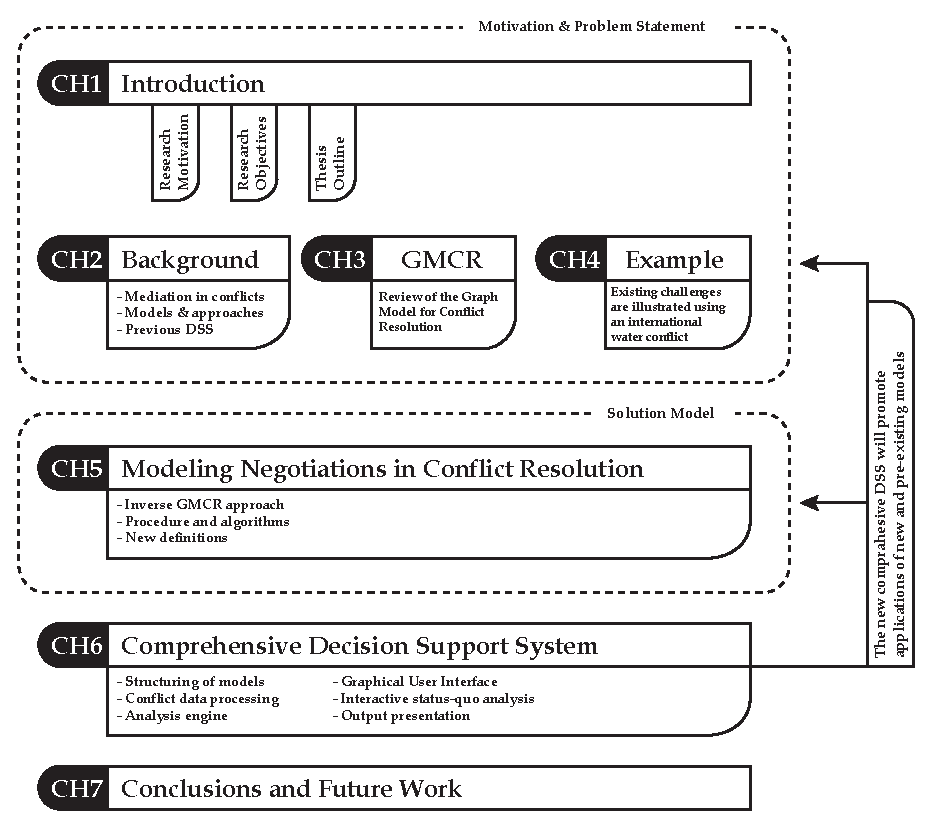
\includegraphics[scale=.8]{PDF-IMG/Thesis_Outline.pdf}

\caption{Thesis Organization}

\label{fig:proposal}
\end{figure}
\end{center}


%======================================================================

% % % Literature % % %


\chapter{Background and Literature Review}
\label{sec:Background}

%%%%%%%%%%%%%%%%%%%%%%%%%%%%%%%%%%%%%%%%%%
%%%%%%%%%%%%%%%%%%%%%%%%%%%%%%%%%%%%%%%%%%


\section{Third Party in Conflicts}


Of the many approaches to the study of third party intervention, three are prominent in the literature \citep{bercovitch2009} :

\begin{enumerate}
\item Individual case studies: these lines of research, such as will be mentioned in the literature review in Chapter 2, analyze and explore specific conflicts in detail. Although this kind of analysis provides significant insights about a particular conflict, it may lack the ability to be generalized and accommodate other conflicts.
\item Experimental approaches: these approaches are laboratory experiments where variables are controlled by researchers in an artificial setting \citep{rubin1980,carnevale2005}
\item Large scale systematic studies: these studies analyze data representing many conflicts and use criteria to identify factors and relationships affecting the conflicts and their outcomes. It gives a more generalized understanding of conflict management.

\end{enumerate}

The methodology presented in this proposal borrows features from the last two approaches. It has controlled variables, yet it is applicable to real conflicts. This methodology is a generalized approach on its basic level, but applies to specific conflicts yielding profound insights.


% % % Whole Section Not changed - From Proposal % % %

Research into the impact of a third party in conflict resolution is reviewed in this section. The first subsection discusses the different types of conflict and the impact of third party intervention on them. Subsections \ref{sec:tproles} and \ref{sec:miscissues} discuss the possible roles of a third party, in addition to other issues. Finally, subsection \ref{sec:tpmodel} reviews the existing modeling approaches for third party intervention.

\subsection{Overview and Conflict Types}
\label{sec:ovrct}
Third party intervention in conflicts has been widely investigated from different perspectives. Most of the research lies within the areas of international relations and political sciences. These studies address  issues regarding mediation including methods of intervention \citep{fisher2001}, strategies for intervention \citep{prein1987}, and conditions for successful intervention \citep{regan1996}. 
Conflicts can be classified in a wide variety of ways. In the world of mediation, the differentiation between intrastate and interstate conflicts is usually clear. A study by \citet{regan1996} focuses on success conditions for third party interventions in intrastate conflicts. Another classification by \citet{bercovitch2006} differentiates between high intensity conflicts and low intensity conflicts. Another categorization for conflicts is based on cause, including ethnic, religious, or ideological \citep{regan1996}.  The size of the conflict, or the number of parties involved provides one more means for classification \citep{jehn1997}

\subsection{Third Party Roles}
\label{sec:tproles}
A third party can assume different roles in a conflict. \citet{sakamoto2005} suggested three roles a third party can undertake in a conflict. These roles are commonly assumed when the mediator is not an actual party in the conflict, but is motivated to bring about a more preferred resolution. The suggested three roles are arbitrator, coordinator, and donor. The authors explain each role within a conflict. A third party is an arbitrator if it has the power to restrict or force a stakeholder to accept a certain resolution. If a third party can alter stakeholders' preferences, then it is either a coordinator or a donor. The difference between the last two roles depends on the time of influence of the third party. A coordinator influences the stakeholder to change preferences immediately, while a donor works on the long term \citep{sakamoto2005}. On the other hand, \citet{raiffa1982} classifies third parties as facilitators, mediators, arbitrators, or rule manipulators. Another study suggests mediators can be individuals, regional organizations, states, or international institutions \citep{bercovitch2000,bercovitch2006}. The latter study surveyed 2,354 international conflicts involving mediation since 1945 in order to analyze them and assess various general hypotheses. Table \ref{tbl:tmad} summarizes their dataset. Some of their hypotheses will be outlined in subsection 2.1.4 of this proposal. 

\begin{center}
\begin{table}[h!]
\centering
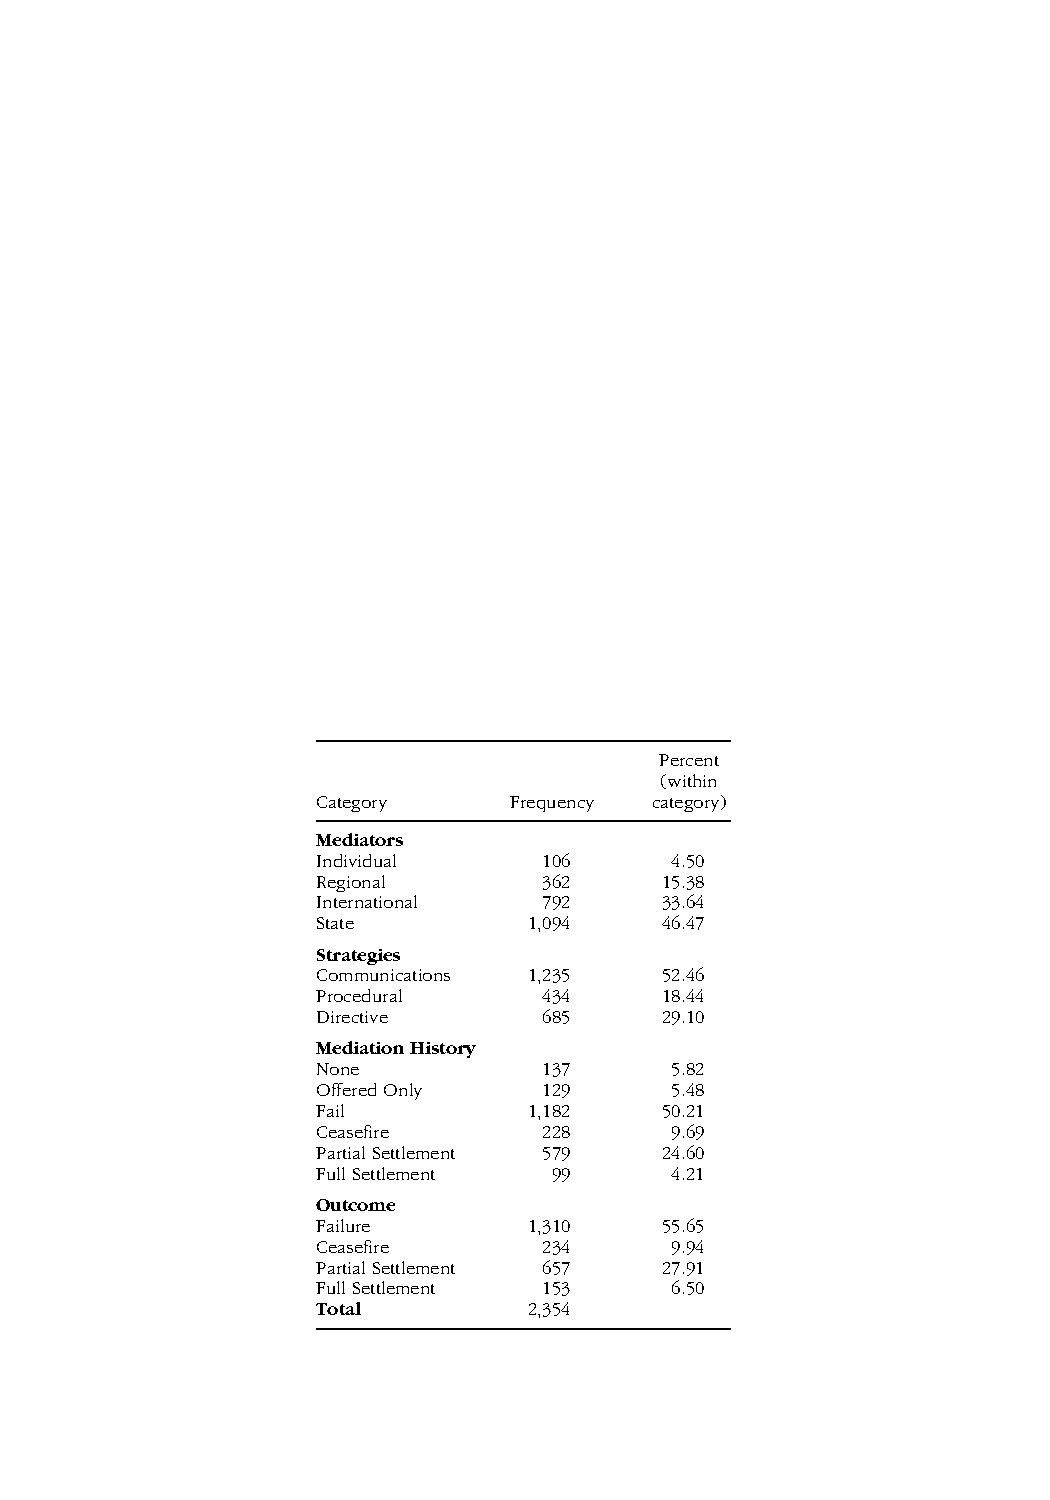
\includegraphics[scale=1]{PDF-IMG/table_mad.pdf}

\caption{Dataset Summary (Adopted from \citet{bercovitch2006}}

\label{tbl:tmad}
\end{table}
\end{center}

\subsection{Miscellaneous issues}
\label{sec:miscissues}
The literature is full of issues and factors affecting third party intervention. For example, factors affecting the process of intervention is that a mediator can act formally or informally, be invited to the conflict or not, intervene independently or on behalf of an organization, have interest in the outcome or in the process of intervention, be inclined toward one party or the other, and be consultative or directive in the intervention \citep{lewicki1992}. Furthermore, mediation history can also have an effect on a new intervention attempt \citep{bercovitch2006}. A study by \citet{carnevale2005} addresses the element of time. They found that time pressure affects the mediator to be aggressive in intervening and to use pressuring tactics. Other studies on the effectiveness of third party intervention suggest factors that influence the success of specific situations. For instance, if an uninvited third party intervenes, \citet{murray1983} specifies three important factors for mediation efficiency: dispute maturity, disputants' relationship, and intervention timing. Other issues raised by different researchers include culture, power asymmetries, conflict ripeness, number of third parties, third party authority, bias, and consistency \citep{fisher2001}.

Another aspect of mediation is strategy. The range of strategies a mediator can undertake is immense. \citet{regan1996} suggests three basic strategies of intervention within intrastate conflicts: military, economic, or mixed. \citet{young1972} discusses four intermediary functions: informational, tactical, supervisory, and re-conceptualization. In another study on successful mediation, \citet{bercovitch1991} outline different strategies that can be adopted by a third party: conciliation-facilitation, procedural, directive, substantive, and supervisory. The authors explain each of these strategies and assess their impact based on a range of historical conflicts. While these studies emphasize specific strategies, other approaches provide a more generic context, referred to as intervention styles. For instance, \citet{bartunek1975} organize intervention techniques into two broad styles: content form and process form. Another wide classification is that of Touval and Zartman, who categorize all intervention approaches as communication, formulation, or manipulation strategies \citep{bercovitch1993}.  \citet{bercovitch2006} suggest that all strategies can be grouped into communication, procedural, or directive strategies.

\subsection{Third Party Modeling}
\label{sec:tpmodel}
Many studies in the literature tackle third party intervention in the context of a specific historical conflict or set of conflicts such as the work by \citet{regan1996,bercovitch1991,dixon1996}.  For instance, the research by \citet{regan1996} on success conditions for third party interventions focuses only on intrastate conflicts and analyzes the conflicts occurred during the period between 1944 to 1994 (Table \ref{tbl:reganset}). The author suggests a regression model based on the dataset he gathered as illustrated in Fig \ref{fig:regansnap}.  The author emphasizes three intrastate conflict types: ethnic, religious, and ideological. Moreover, the regression model took into account other factors affecting the intervention such as the type of conflict, number of causalities, intervention type, and intervention target.
Other attempts to formally model third party intervention based on particular conflicts include the research by \citet{carment1996,HipelRami}. Although most third party modeling based on historical conflicts use regression analysis \citep{regan1996,dixon1996}, the latter two studies use game theory based models. In addition, \citet{fisher2001,lewicki1992} discuss different conceptual and descriptive models for third party intervention. Lastly, a standard conflict model of third party intervention is suggested by \citet{siqueira2003}.


\begin{center}
\begin{figure}[H]
\centering
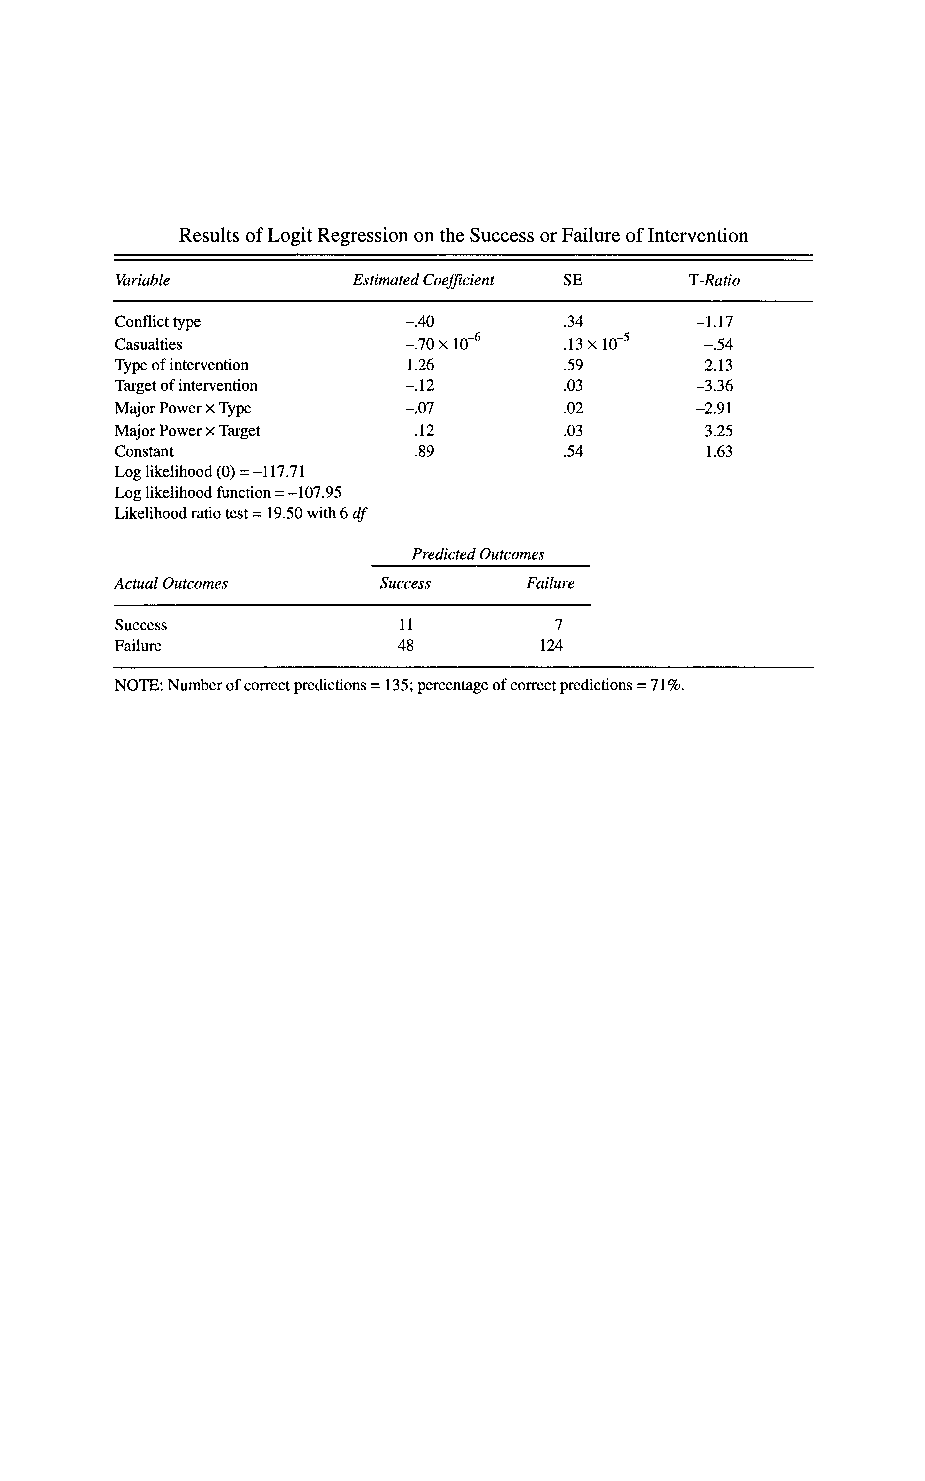
\includegraphics[scale=1]{PDF-IMG/Regan_snap.pdf}

\caption{A snapshot of the regression model by \citet{regan1996} with the results applied to the study dataset}

\label{fig:regansnap}
\end{figure}
\end{center}

\begin{center}

\begin{table}[H]
\centering
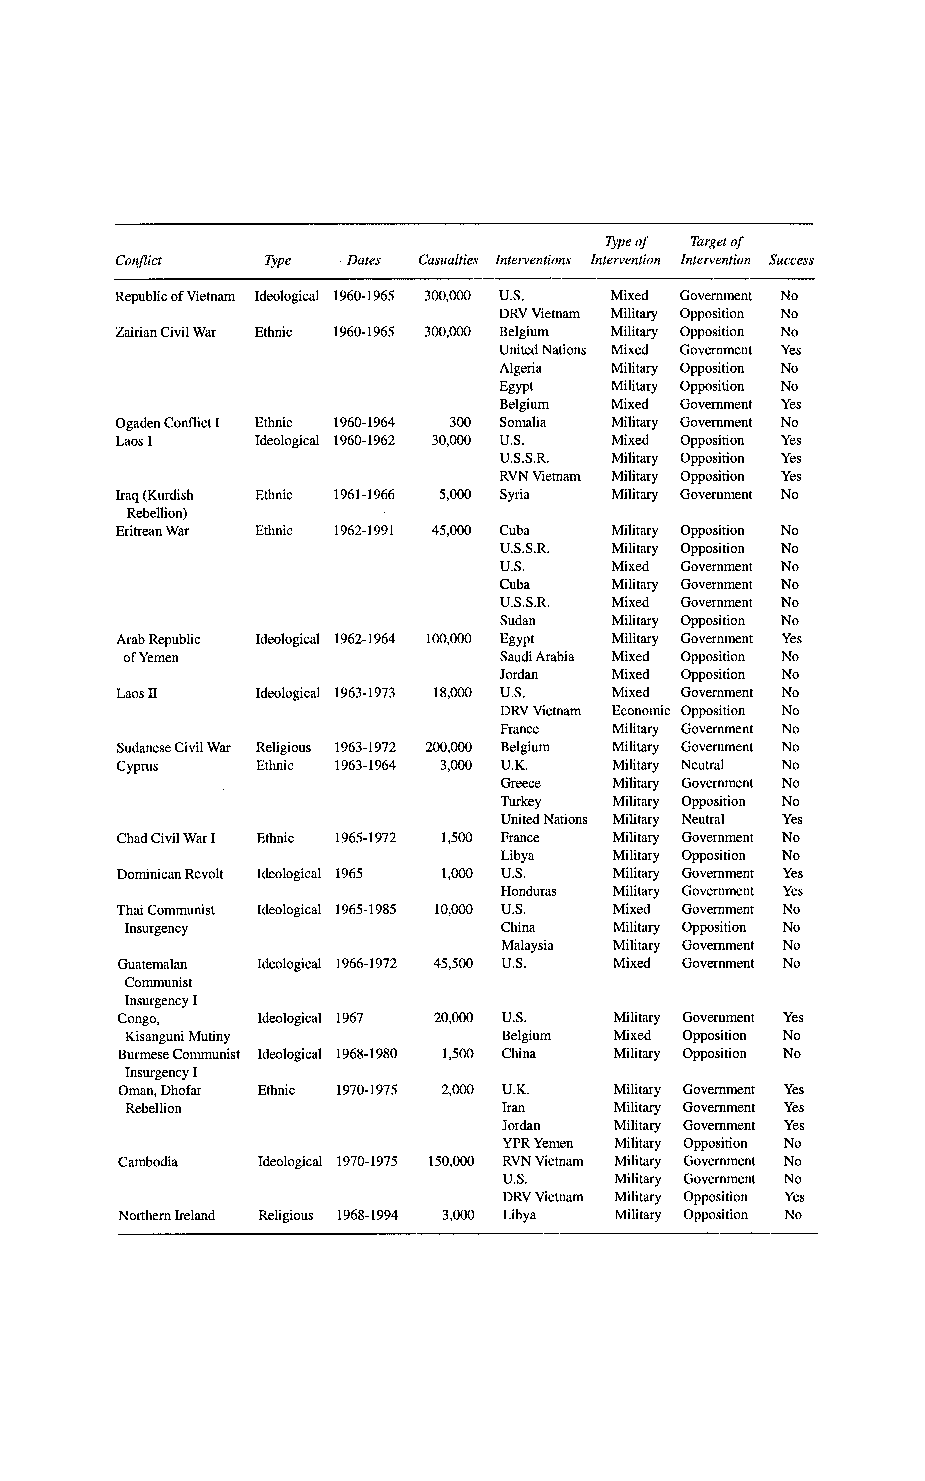
\includegraphics[scale=1]{PDF-IMG/Regan_set.pdf}

\caption{A dataset segment of the Intrastate Conflicts used in Regan's study (Table adopted from \citet{regan1996}}

\label{tbl:reganset}
\end{table}

\end{center}


A study by \citet{sakamoto2005} illustrates an approach to incorporate third party intervention in conflict modeling using GMCR. The research suggests three roles a third party can play (explained in subsection 2.1.2 of this report) and developed a conflict management procedure for them. Fig \ref{fig:sakamato_flow} below illustrates the authors' conflict management approach with the intervention of a third party.

\begin{center}
\begin{figure}[H]
\centering
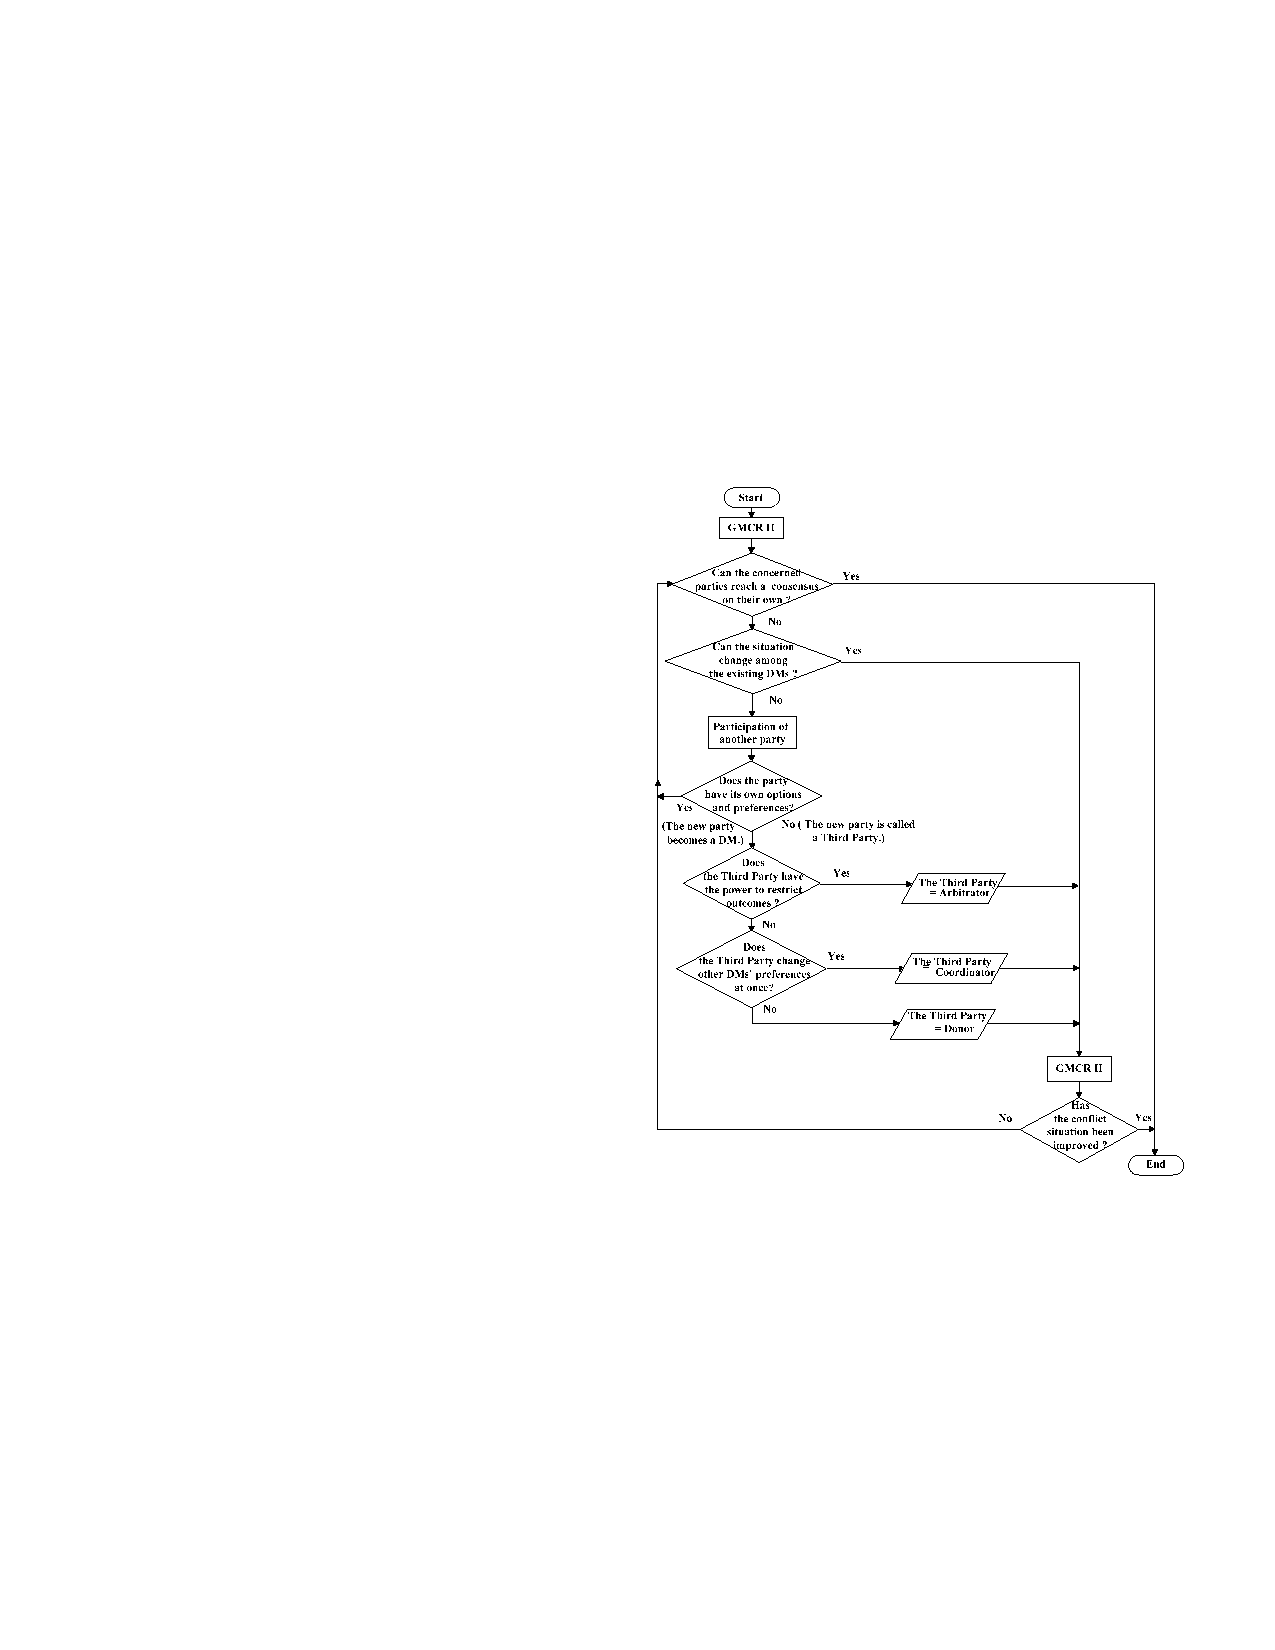
\includegraphics[scale=1]{PDF-IMG/sakamato_flow.pdf}

\caption{Chart developed by \citet{sakamoto2005} to illustrate conflict management with a third party}

\label{fig:sakamato_flow}
\end{figure}
\end{center}

A comprehensive study by \citet{bercovitch2006} investigates in depth the success factors of third party intervention. The authors focus on mediators' identities, strategies, and mediation history to predict the outcome of mediation. According to the authors, mediators can be classified according to four categories: individuals, states, regional organizations, and international institutions. After discussing each category, the authors claim that in low intensity conflicts, state and regional mediators are more likely to be successful. However, they are less likely to be successful in high intensity conflicts. International mediators are likely to be effective in high intensity conflicts and individuals are unlikely to be successful in all conflict types.
On the other hand, the authors suggest that mediation strategies include communication-facilitation, procedural, and directive strategies. Similarly, the authors make some hypotheses after explaining each of the strategies. They claim that directive strategies are most likely to be successful in high intensity conflicts but not in low intensity conflicts. Procedural strategies are mostly successful in low intensity conflicts. Tables \ref{tbl:MEDIATOR_TYPE} and \ref{tbl:MEDIATOR_STR} are summaries derived from the research hypotheses in the study. 

\begin{center}

\begin{table}[H]
\centering
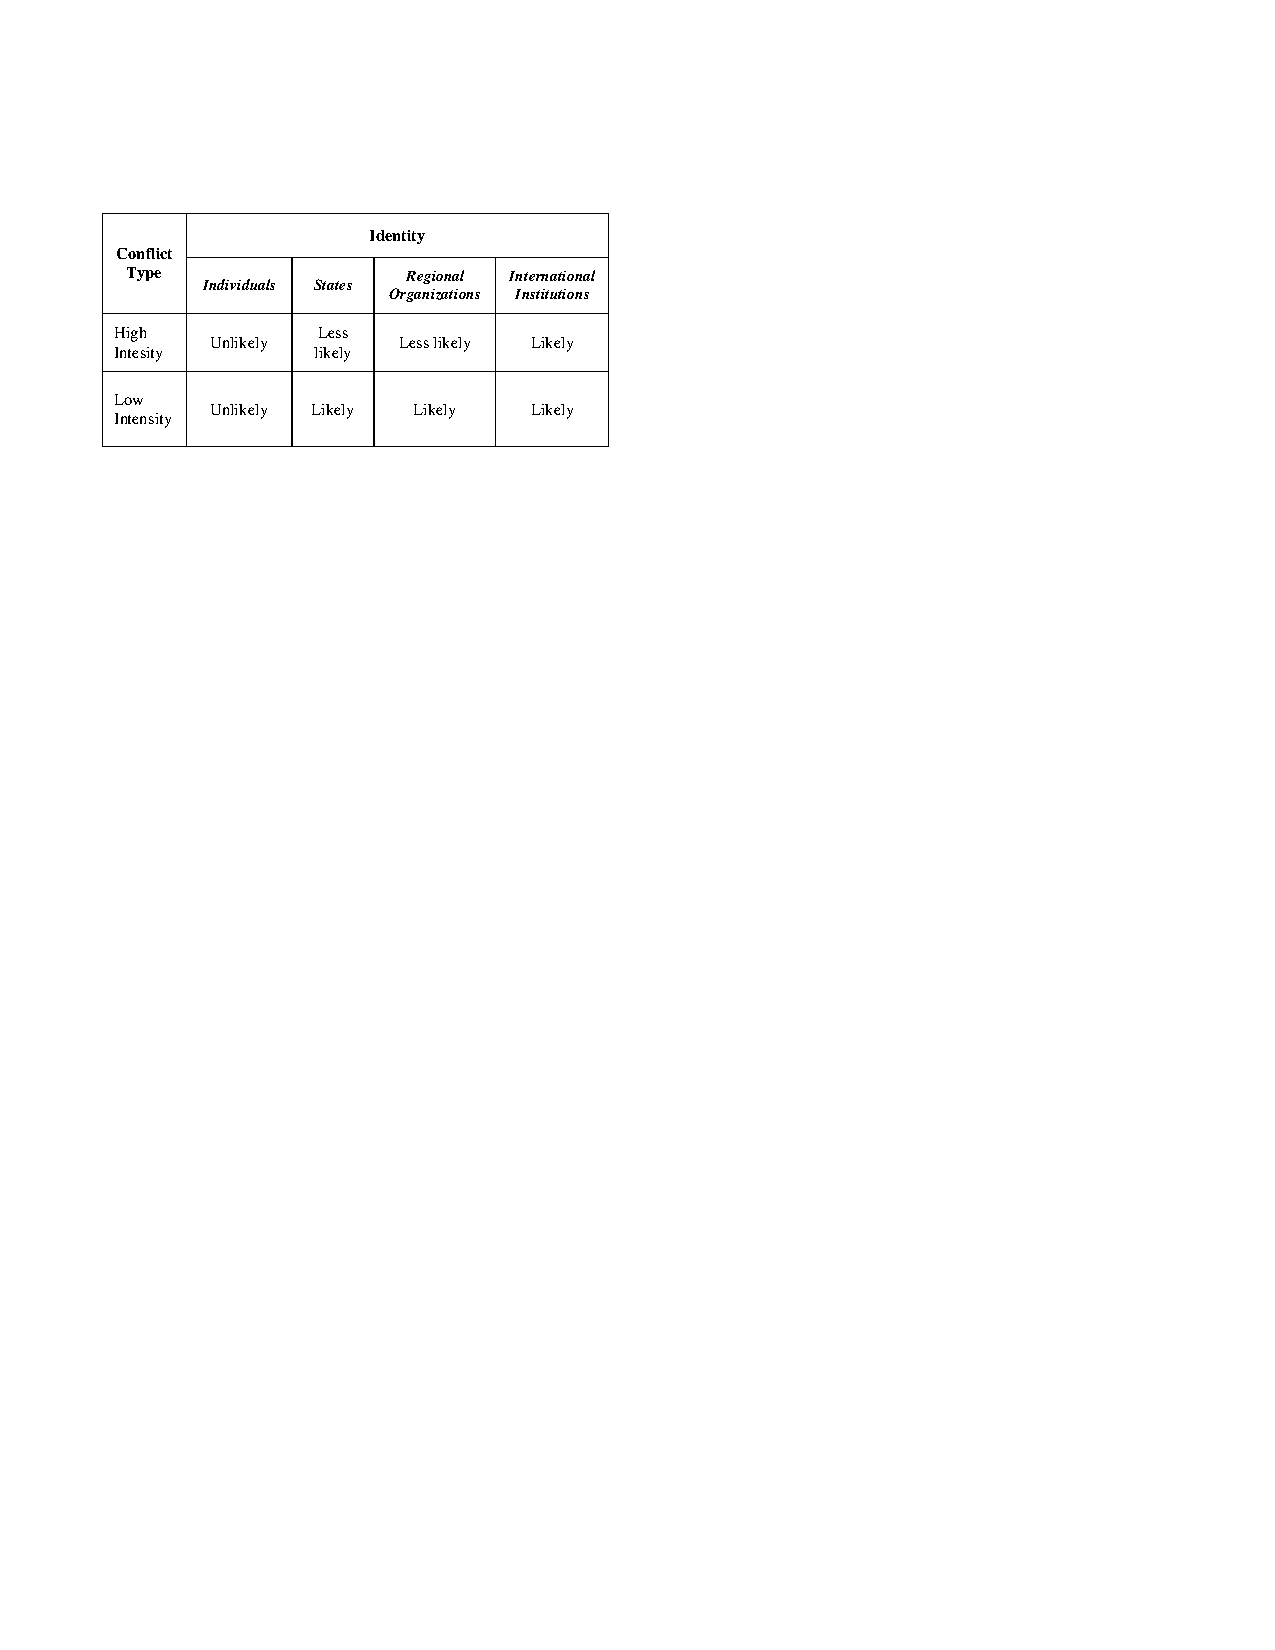
\includegraphics[scale=1]{PDF-IMG/MEDIATOR_TYPE.pdf}

\caption{Mediator type and likelihood to be successful}

\label{tbl:MEDIATOR_TYPE}
\end{table}

\end{center}

\begin{center}

\begin{table}[H]
\centering
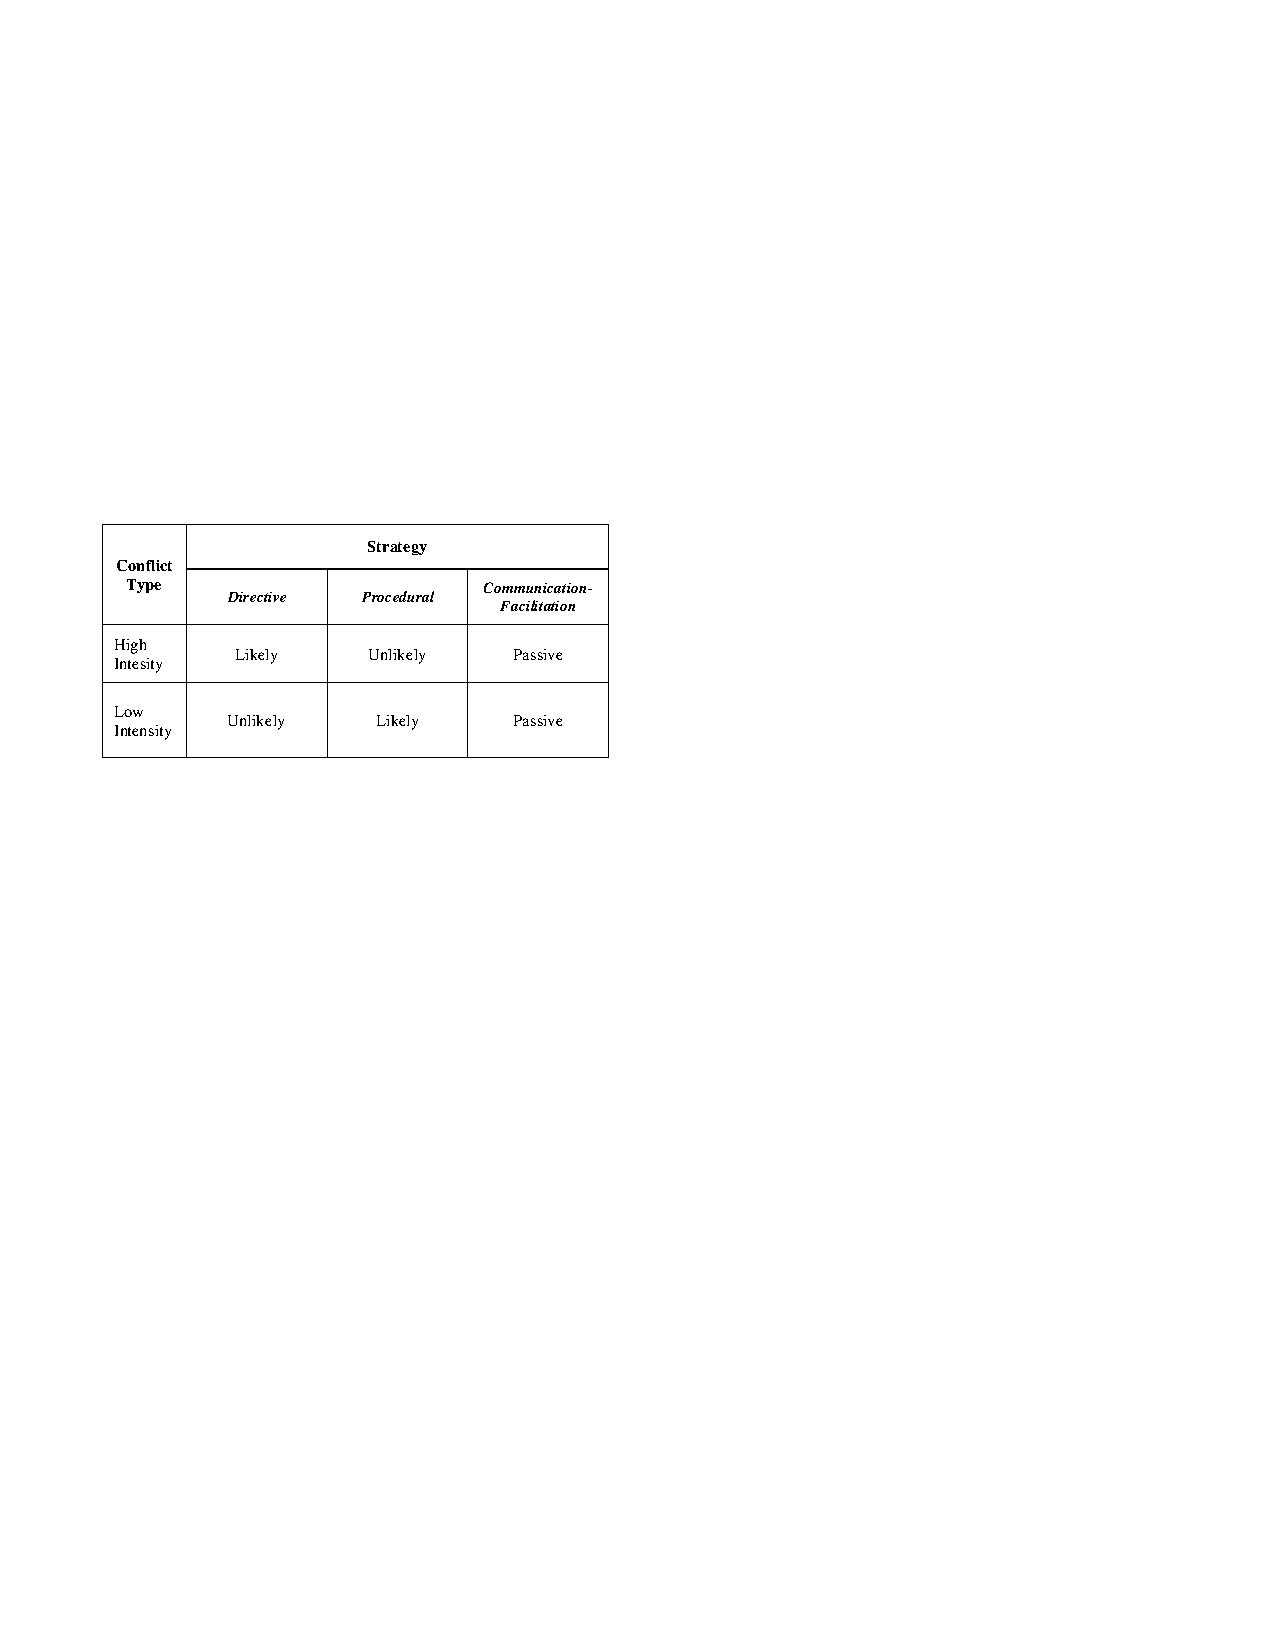
\includegraphics[scale=1]{PDF-IMG/MEDIATOR_STR.pdf}

\caption{Mediator strategy and likelihood to be successful}

\label{tbl:MEDIATOR_STR}
\end{table}
\end{center}

\section{Models and Approaches}

In order to formally model third party intervention in conflicts, three areas will be investigated, as follows:
\begin{enumerate}
\item Inverse approach to conflict resolution: A modeling technique that will allow mediators to choose a desired outcome as equilibrium, and work backwards to achieve it.
\item Inverse status quo analysis: An extension to the previous area that determines whether the desired equilibrium is reachable from the original state.
\item Third party prediction: A tool to analyze conflicts inviting mediation and give insight as to which role a mediator should play to resolve the conflict.

\end{enumerate}

\section{Chapter Summary}

%%%%%%%%%%%%%%%%%%%%%

\chapter{The Graph Model for Conflict Resolution (GMCR)}
\label{sec:GMCR}
The Graph Model for Conflict Resolution (GMCR) has been developed and expanded since the mid-1980s \citep{kilgour2005}. GMCR is a tool to strategically analyze moves and counter moves in a conflict in order to predict the most likely outcome. 
\section{Procedure}
The basic procedure of GMCR involves two main stages: modeling and analysis. In the modeling stage, the user identifies the conflict parameters which include:
\begin{itemize}
\item Decision makers (DMs)
\item Options for each DM
\item Infeasible states (such as mutually exclusive situations)
\item Allowable transitions
\item Relative preferences
\end{itemize}

After identifying the conflict parameters, the user will analyze the conflict from each DM's perspective to determine the likely final resolution. This stage include:
\begin{itemize}
\item Determining individual stability (i.e. for each DM)
\item Overall equilibria
\item Sensitivity analysis
\end{itemize}

The following diagram in Figure \ref{fig:procedure_or} illustrates the basic GMCR procedure (The diagram is adapted from \citet{fang1993}).

\begin{center}
\begin{figure}[h!]
\centering
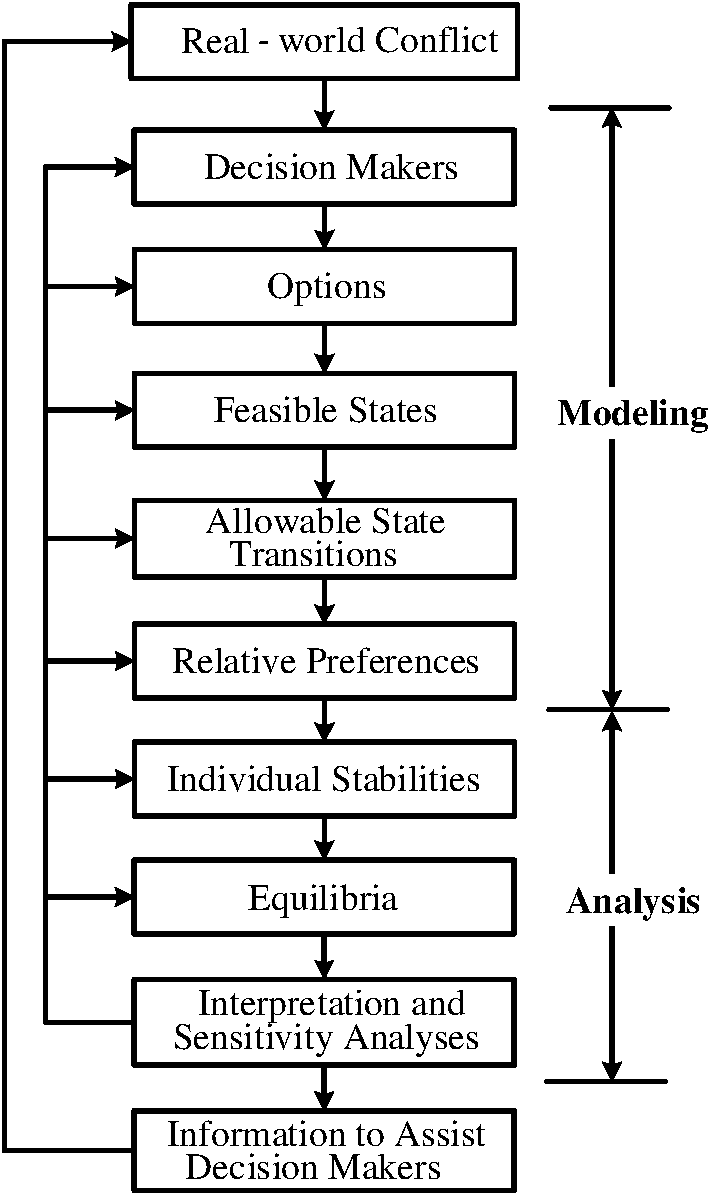
\includegraphics[scale=0.65]{PDF-IMG/GMCR_pro.pdf}

\caption{The basic procedure of GMCR in a real world conflict (adapted from \citet{fang1993})}

\label{fig:procedure_or}
\end{figure}
\end{center}

\section{Notation and Definitions}
The graph model representing a real world conflict includes DMs, options, and preferences. These parameters are formally defined as follows:

\begin{definition}
\rm
Let $N=\{1,2,\dots,n\}$ represent the set of DMs, for each DM $i \in N$, the set $O_{i}$ is $i$'s options or strategy set and $S=\{s_1, s_2, ..., s_m\}$ represent the set of feasible states.
\end{definition}

The set of possible states in a conflict is represented by the expression $2^o$ where $o$ is the total number of options in a conflict. Some of the possible states may be infeasible such as mutually exclusive options, at least one type of options, or dependent options. In a conflict model, a set of feasible states is defined.
%Cartesian product $S_{1} \times S_{2} \times \dots \times S_{n}$

\begin{definition}
\rm
Let  $S=\{s_1, s_2, ..., s_m\}$ represent the set of feasible states in a conflict. For each DM $i \in N$, a set of directed graphs $D_{i}=(S,A_{i})$ can be used to model the conflict.
\end{definition}


The feasible states of a conflict are represented by vertices in the graph model. In each graph, an arc $A_{i}$ exists between states $s_a$ and $s_b$ $\in$ $S$ if DM $i$ can move unilaterally in one step between the two states. It is called a \emph{directed} graph because the arc has an orientation which can be one way (irreversible move) or two ways (reversible move).

\begin{definition}
\rm
Let $i \in N$ and $s \in S$. The reachable list of DM $i$ from state $s \in S$ is defined as:
$$R_i(s)=\{s_a \in S \quad : \quad (s, s_a) \in A_i\}$$
\end{definition}

The move in one step by DM $i$ from a state $s_a$ to a state in the reachable list $\{s_b\in S\}$ is called a unilateral move (UM).

The preference information of DM $i$ is a binary relation $\{\succ_i,\sim_i\}$ over $S$, where $s_a\succ_i s_b$ means that DM $i$ prefers $s_a$ to $s_b$ and $s_a\sim_i s_b$ means that DM $i$ is indifferent between states $s_a$ and $s_b$. The binary relation $\{\succ_i,\sim_i\}$ is considered complete.

\begin{definition}
\rm
Let $i \in N$ and $s \in S$. The unilateral improvement list for DM $i$ from state $s \in S$ is defined as:
$$R_i^+(s)=\{s_a \in R_i(s) \quad : \quad s_a\succ_i s\}.$$
\end{definition}

The move in one step by DM $i$ from a state $s_a$ to a state in the unilateral improvement list $\{s_b\in S\}$ is called a unilateral improvement (UI).

\section{Stability Definitions and Solution Concepts}
\label{sec:stability}
The main goal of the graph model for conflict resolution is to predict the stability of each state for each DM. There are four basic solution concepts according to which a state can be assessed for stability: Nash stability (sometimes called rationality), sequential stability (SEQ), general metarationality (GMR), and  symmetric metarationality (SMR). 

The solution concepts describe how a DM is motivated to make moves and counter moves. These concepts (or behavior patterns) determine whether a specific state will be terminal or a DM will be motivated to deviate to another state. Different DMs may have different behavior patterns based on different factors. These factors include risk, foresight, and available information. Behavioral characteristics according to the different solution concepts are given in Table \ref{tbl:behchar} below. 

\begin{definition}
\rm {\bf (Nash Stability)} Let $i \in N$ and $s \in
S$. State $s$ is \emph{Nash stable} for DM $i$ \emph{iff} $R_i^+(s)=\phi$.
\end{definition}

\begin{definition}
\rm {\bf (Sequential Stability)} Let $i \in N$ and $s \in
S$. State $s \in S$ is \emph{sequentially stable} (\emph{SEQ}) for DM $i$ \emph{iff} for every $s_1 \in R_i^+(s)$ there exists at least one $s_2 \in R_{N-i}^+(s_1)$
such that $s_2 \precsim_i s$.
\end{definition}

\begin{definition}
\rm {\bf (General Metarationality)} Let $i \in N$ and $s \in
S$. State $s \in S$ is \emph{general metarational} (\emph{GMR}) for DM $i$ \emph{iff} for every $s_1 \in R_i^+(s)$ there exists an $s_2 \in
R_{N-i}(s_1)$ such that $s_2 \precsim_i s$.
\end{definition}

\begin{definition}
\rm {\bf (Symmetric Metarationality)}  Let $i \in N$ and $s \in
S$. State $s \in S$ is \emph{symmetric metarational} (\emph{SMR}) for DM $i$ \emph{iff} for every $s_1 \in R_i^+(s)$ there exists an $s_2 \in
R_{N-i}(s_1)$ such that $s_2 \precsim_i s$ and $s_3 \precsim_i s$
for all $s_3 \in R_k(s_2)$.
\end{definition}

\begin{table}[H]
\centering
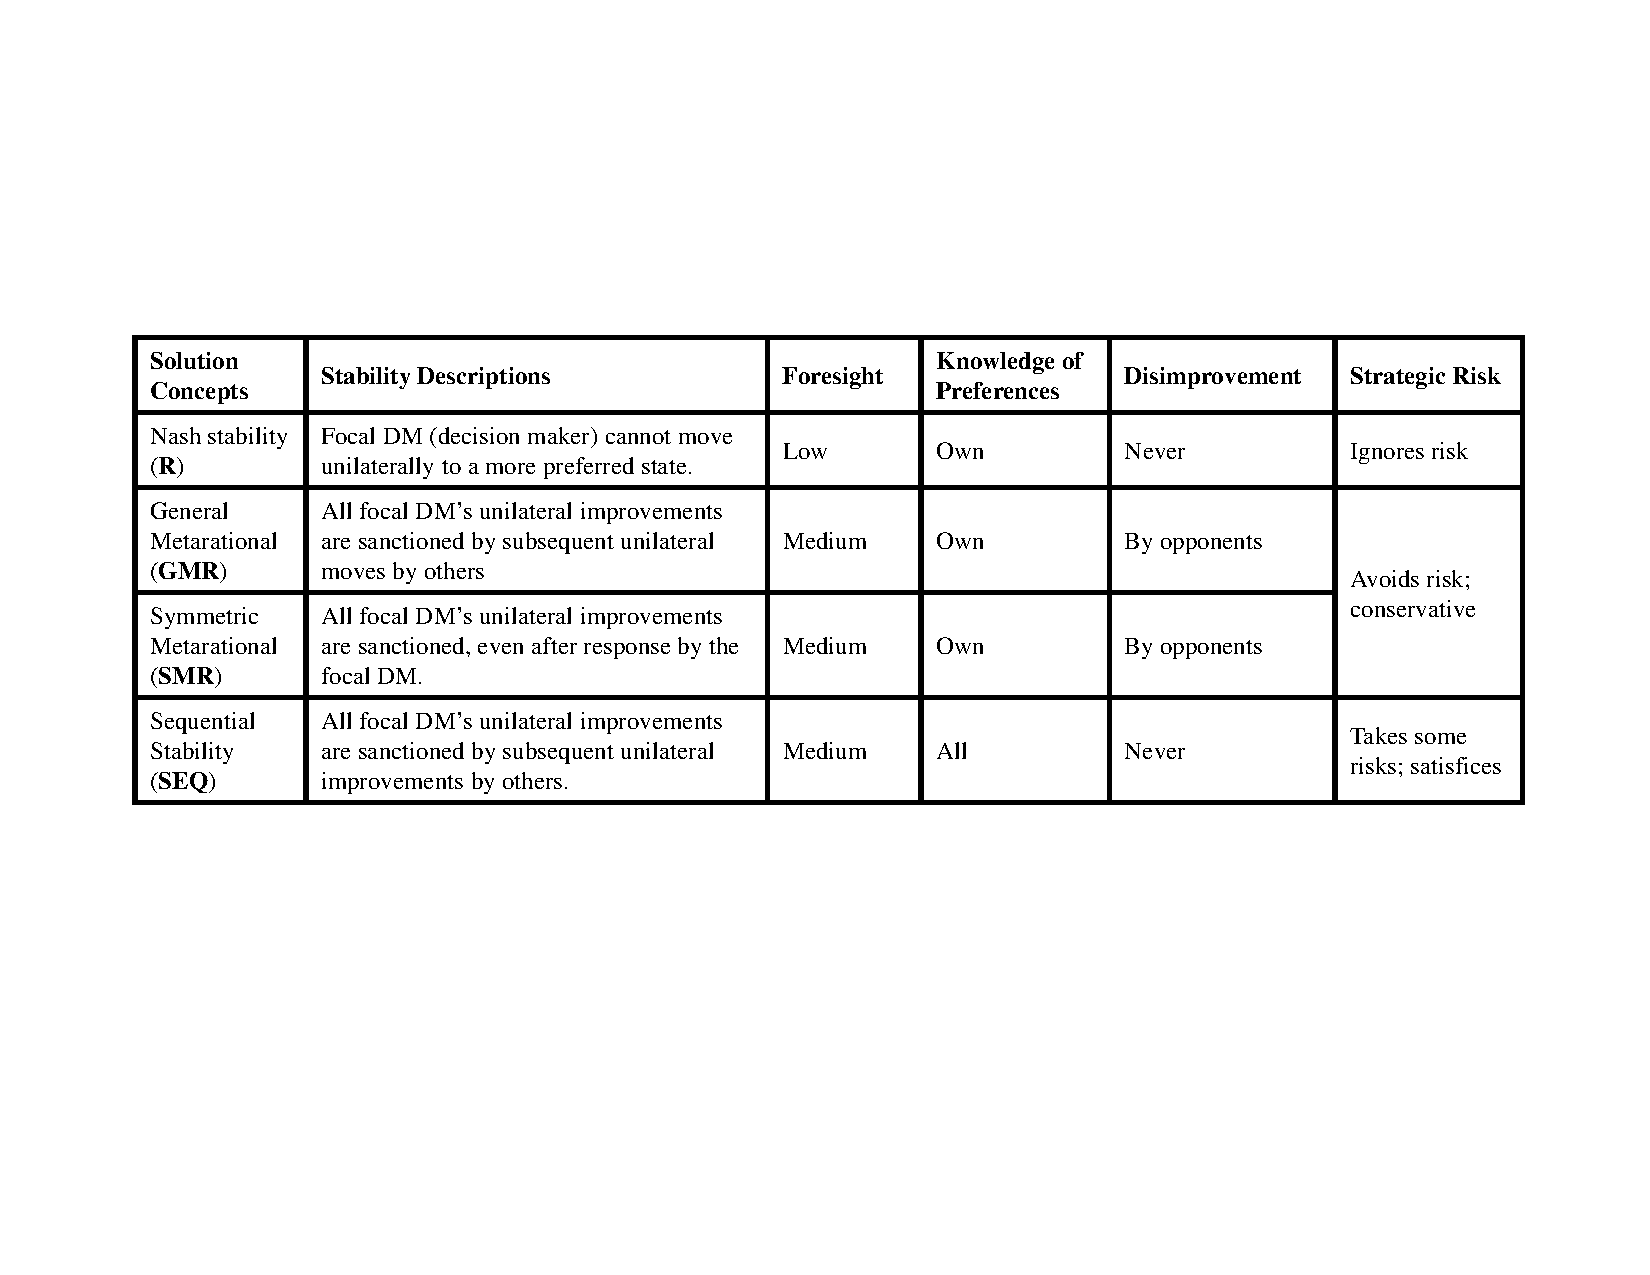
\includegraphics[scale=.75]{PDF-IMG/tablecomp.pdf}

\caption{Behavioral characteristics describing different solution concepts}

\label{tbl:behchar}
\end{table}

\begin{definition}
\rm {\bf (Equilibrium)}  Let $i \in N$ and $s \in
S$. State $s \in S$ is called \emph{equilibrium} (\emph{E}) \emph{iff} it is stable for every DM.
\end{definition}

Sometimes the graph model for conflict resolution is referred to as a 3-tuple or triplet $G=\langle N,S,(\succ_i,\sim_i)_{i\in N}\rangle$ where $N$ is the list of DMs $N=\{1,\dots ,n\}$, $S$ is the set of feasible states $S=\{1,\dots ,m\}$, and $(\succ_i,\sim_i)$ is the binary relation DM $i$ has on $S$. Consequently, $Nash(G)=\{ \enskip s \in S \enskip : \enskip s \enskip$  is a Nash Equilibrium of $G \}$. More explicitly, $$Nash(N,S,(\succ_i,\sim_i)_{i\in N})=\{ \enskip s \in S \enskip : \enskip s \enskip  \text{is Nash stable for all } i \in N \text{ in } \langle N,S,(\succ_i,\sim_i)_{i\in N}\rangle \}$$ and similarly for SEQ, GMR, and SMR.

%%%%%%%%%%%%%%%%%%%%%

\section{Follow-Up Analysis}

To take the basic analysis further, a number of follow-up analyses may be undertaken to test the reliability of the predicted outcomes and whether they are achievable from the status quo or not.

\subsection{Sensitivity Analysis}

Since many conflict parameters are subjective, it may be essential to test different scenarios in order to determine the robustness of the conflict model. Sensitivity analysis also points out how different parameters can influence the stability results. The most common type of sensitivity analysis is the change of preference since it is the most difficult parameter to obtain and determine. Other sensitivity analysis types include:

\begin{itemize}
\item Adding or combining DMs
\item Change of options (adding, removing, or modifying) 
\item Changing moves reversibility
\item Coalition analysis
\item Modeling misunderstandings (hypergames)
\item Examining other patterns of human behavior
\end{itemize}

%%%%%%%%%%%%%%%%%%%%%

\subsection{Status Quo analysis}

Every real world conflict has a starting point from which the conflict evolves. This point or state is called \emph{status quo} \citep{fang1993}. Depending on the status quo, a potential equilibrium may or may not be reached. \citet{li2004squo,li2005squo} developed algorithms and formal definitions to inspect the attainability of a potential resolution (\emph{equilibrium}) from a certain state (\emph{status quo}).

\section{Decision Support System for GMCR}

\subsection{Review of Existing Decision Support Systems}

\section{Chapter Summary}

%%%%%%%%%%%%%%%%%%%%%

\chapter{Strategic Investigations of Water Conflicts in the Middle East}
\label{sec:example1}

The arid nature of the Middle East environment causes continuously escalating conflicts among the countries of the region. Conflicts arise as water resources dwindle due to increased industrial and agricultural projects and population growth. The main renewable sources of freshwater in the region are rivers. Like all water resources, they are replenished by their hydrological cycle, with renewal rates varying from days to centuries. The rate of renewal for Middle Eastern rivers is decreasing due to population growth and the increasingly arid conditions of the region. At 2,700 km, the Euphrates is the longest and arguably most important river in the Middle East (Southwest Asia) \citep{kolars1991euphrates}.
The Euphrates originates in eastern Anatolia in Turkey and flows through Syria and finally Iraq, where it joins the Tigris River. Conflicts regarding the river became serious during the 1960s, when Turkey began building dams on the Euphrates to generate electricity and increase the availability of irrigation water in Southeast Turkey \citep{akanda2007tigris}. As a result of external mediation, war was narrowly avoided twice, in 1975 and 1998 \citep{akanda2007tigris}.

Water conflicts have been widely investigated during the last decade \citep{dinar2004exploring} and different approaches taken to model them \citep{madani2010game}. For instance, the Waiahole Water Project conflict, in the American state of Hawaii,  has been modeled and analyzed using the Graph Model for Conflict Resolution \citep{gopalakrishnan2005water}, and a status quo analysis of the Flathead River conflict involving the United States and Canada was examined using the same methodology \citep{Li2004flathead}. Other modeling approaches used for studying water conflicts include Alternative Dispute Resolution (ADR) \citep{wolf2000indigenous}, Shared Vision Modeling \citep{lund1997water}, and Adjusted Winner (AW) mechanism \citep{massoud2000fair}.

The aim of this chapter is to examine in depth the main conflicts that have occurred in the past along the Euphrates and to model them using the GMCR methodology \citep{Kilgour1987,fang1993} as implemented by the decision support system, GMCR II \citep{hipel1997decision,fang2003a,fang2003b}. Time periods of interest for this analysis are 1975, 1990, and 1998, when the conflict escalated to the near outbreak of a full scale war. Accordingly, the historical backgrounds underlying the disputes at these three points in time are described in the next section. Subsequently, modeling and stability analyses are carried out for these three conflicts, followed by a summary of strategic insights that are garnered.



\section{Background}

As explained in the next three subsections, the interconnected conflicts of 1975, 1990, and 1998 took place dynamically over time. Therefore, systematically investigating these disputes together enhances the appropriateness of the analyses and furnishes more meaningful insights.

\subsection{The conflict in 1975}
\label{Conflict1975}
In 1966, Turkey started the construction of the Keban Dam, which is a hydroelectric dam on the Euphrates River (Fig \ref{fig:dams}). After the construction was finished in 1974, Turkey started the filling of the Keban Reservoir. During the flooding, Turkey maintained a 450 $m^3/s$ discharge of the Euphrates to the two downstream countries consisting of Syria and Iraq. This rate was agreed upon by both countries through the United States Agency for International Development (USAID), which was financing the project \citep{inan2000law}. However, Syria also started filling the lake behind its newly constructed Thawra Dam. Simultaneously, the area was hit by a significant drought \citep{kalpakian2004identity}. As a result, the flow of the Euphrates River entering Iraq was reduced to a trickle. Iraq accused Syria of this reduction and of endangering the lives of three million Iraqi farmers dependent on river irrigation water \citep{morris1997water}. Iraq complained that the flow had dropped from the normal 920 $m^3/sec$ to an unacceptable 197 $m^3/sec$ \citep{priscoli2009managing}. Iraq requested an intervention by the Arab League; however, Syria argued that it was receiving less water from Turkey as well and refused to cooperate. As the tension increased, Syria closed its airspace to all Iraqi aircraft, suspended Syrian flights to Baghdad, and transferred troops from the Israeli border to the Iraqi frontier by May 1975 \citep{morris1997water}. Iraq also sent its troops to the shared border and threatened to bomb Syria's dam. 

Before the conflict could escalate any further, Saudi Arabia and the Soviet Union intervened - only mediation on the part of Saudi Arabia was able to alleviate the situation \citep{priscoli2009managing}. On June 3, 1975, an agreement between Iraq and Syria, with the mediation of Saudi Arabia, averted the impending war. The agreement stipulated that Syria is to release extra amounts of water to Iraq \citep{akanda2007tigris}: specifically, 58\% of what Syria receives from the Euphrates is to be released to Iraq \citep{priscoli2009managing}. In addition to resolving the conflict, Saudi Arabia contributed to a basin fund that would finance irrigation reform and other methods to reduce unmet demands \citep{akanda2007tigris}.

\begin{center}
\begin{figure}[h]
\centering
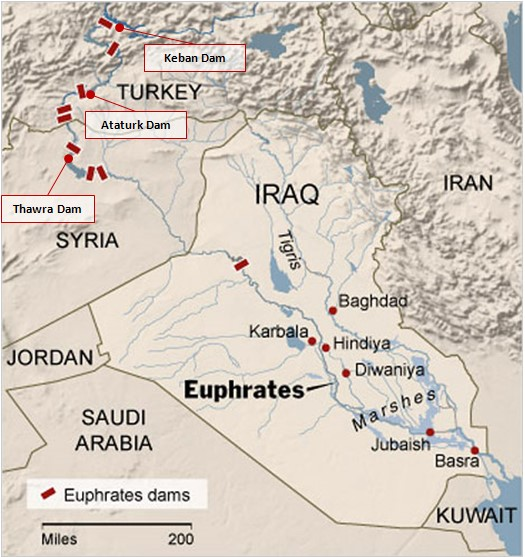
\includegraphics[scale=.6]{PDF-IMG/dams.jpg}

\caption{The Euphrates River along with the dams constructed on it (The New York Times, 2009)}

\label{fig:dams}
\end{figure}
\end{center}

\subsection{The Conflict in 1990}
In 1977, Turkey announced plans for the largest water resources project in South-Eastern Anatolia, referred to as ``G�neydogu Anadolu Projesi", commonly known as the ``GAP Project", which includes 22 dams and 19 hydropower installations on the Euphrates-Tigris \citep{frenken2009irrigation}. The incentive for this project, apart from the steadily increased water demand, was to promote Turkey?s internal stability. Turkey has been continually preoccupied with the rebellion movement of the Kurdish Workers Party (PKK), which is struggling to create a Kurdish state in South Eastern Turkey \citep{guner1998signalling}. The construction of the GAP project scattered the Kurdish rebels and the PKK denounced the GAP project as harmful to Kurds and their villages. GAP irrigation projects transformed the geography of the area and obstructed the free movement of the PKK. The PKK had targeted the GAP project with sabotage and kidnapping of engineers in order to stop the development. Aside from weakening the PKK movement, the GAP project also provided extra jobs for resident Kurds, thereby promoting internal stability. It also helped in stemming the flow of immigrants from this region to the already over-crowded cities.

On the other hand, both Syria and Iraq demonstrated their distrust and rejection of the GAP project. When Turkey requested funding from the World Bank for a second dam after the Keban Dam, Syria and Iraq raised many objections to urge the World Bank to withhold the funding, although the Bank and Turkey concluded that the downstream requirements could be satisfied \citep{akanda2007tigris}. During the conflict between Turkey and PKK, Syria supported the PKK by granting their leader refugee status and provided him with shelter. Moreover, Syria allowed PKK to have military bases in the Beqaa Valley, a region in eastern Lebanon under Syria?s control \citep{guner1998signalling}. Syrian support of the PKK was potentially intended for the reduction, or at least the interruption, of the GAP project \citep{guner1998signalling}. In 1987, Turkey guaranteed a minimum water flow of 500 $m^3/s$ and Syria, in return, promised to cooperate in security matters. A few months later, Turkey complained about terrorist activities and accused Syria of supporting them \citep{guner1998signalling}. Turkey allegedly hinted at a cut in the flow of Euphrates water to Syria over Syrian support for Kurdish terrorists \citep{starr1991water}. In January 1990, Turkey completely stopped the flow of the Euphrates. The official justification for the interruption was to fill the lake behind the Ataturk Dam and the interruption was intended to be only for one month \citep{darwish1994}. Behind the scenes, this interruption was an indirect threat to Syria for its continued support of the PKK. Turkey did not care about Iraq?s reaction as Syria and Iraq were bitter enemies; however, Turkey?s actions united both Iraq and Syria against it.
Once Turkey halted the flow of the Euphrates, both countries, Syria and Iraq, boycotted companies involved in the GAP project. Furthermore, military leaders from both nations drew up plans for armed retaliation against Turkey \citep{darwish1994}. After three weeks, water was released in the Euphrates River, even though the interruption was intended to last a whole month. 


\subsection{The Conflict in 1998}
After the joint coalition between Syria and Iraq in 1990, Turkey decided not to use the Euphrates as a weapon in order to avoid Iraq?s intervention. However, Syria's continuous support for the PKK was affecting Turkey's stability and depleting its resources. Despite bilateral security agreements between Syria and Turkey in 1992 and 1993, Turkey continued to accuse Syria of supporting the PKK, while Syria insisted that it forced the PKK to move its bases from Syrian territory in conformity with the bilateral agreements between itself and Turkey \citep{guner1998signalling}. In 1993, the Turkish Prime Minister declared that if Syria did not ban PKK from its country, there could be no solution to the water problem. The issue was raised again in the trilateral summit of 1994 between the Foreign Ministers of Turkey, Syria, and Iraq with no improvements. Moreover, in 1995, Turkey organized military operations in northern Iraq against PKK members who fled to Syria, thus confirming Turkish suspicions. Finally, in 1998, Turkey charged Syria with support of the PKK and harboring its leader, perhaps providing refuge to the leader in Damascus. Turkey escalated the situation and threatened to invade Syria. Egypt intervened and the Egyptian President, Hosni Mubarak, secured Syria's pledge to stop supporting the PKK \citep{akanda2007tigris}. On account of the intervention of Egypt and in order to avert an invasion by Turkey, the Syrian government agreed to ban PKK from Syria by signing the Adana Agreement on October 20, 1998 \citep{priscoli2009managing}. Finally, Table \ref{tbl:historyEuphrates} provides the historical evolution of the most notable events related to the Euphrates conflicts.

\begin{table}[H]
\centering
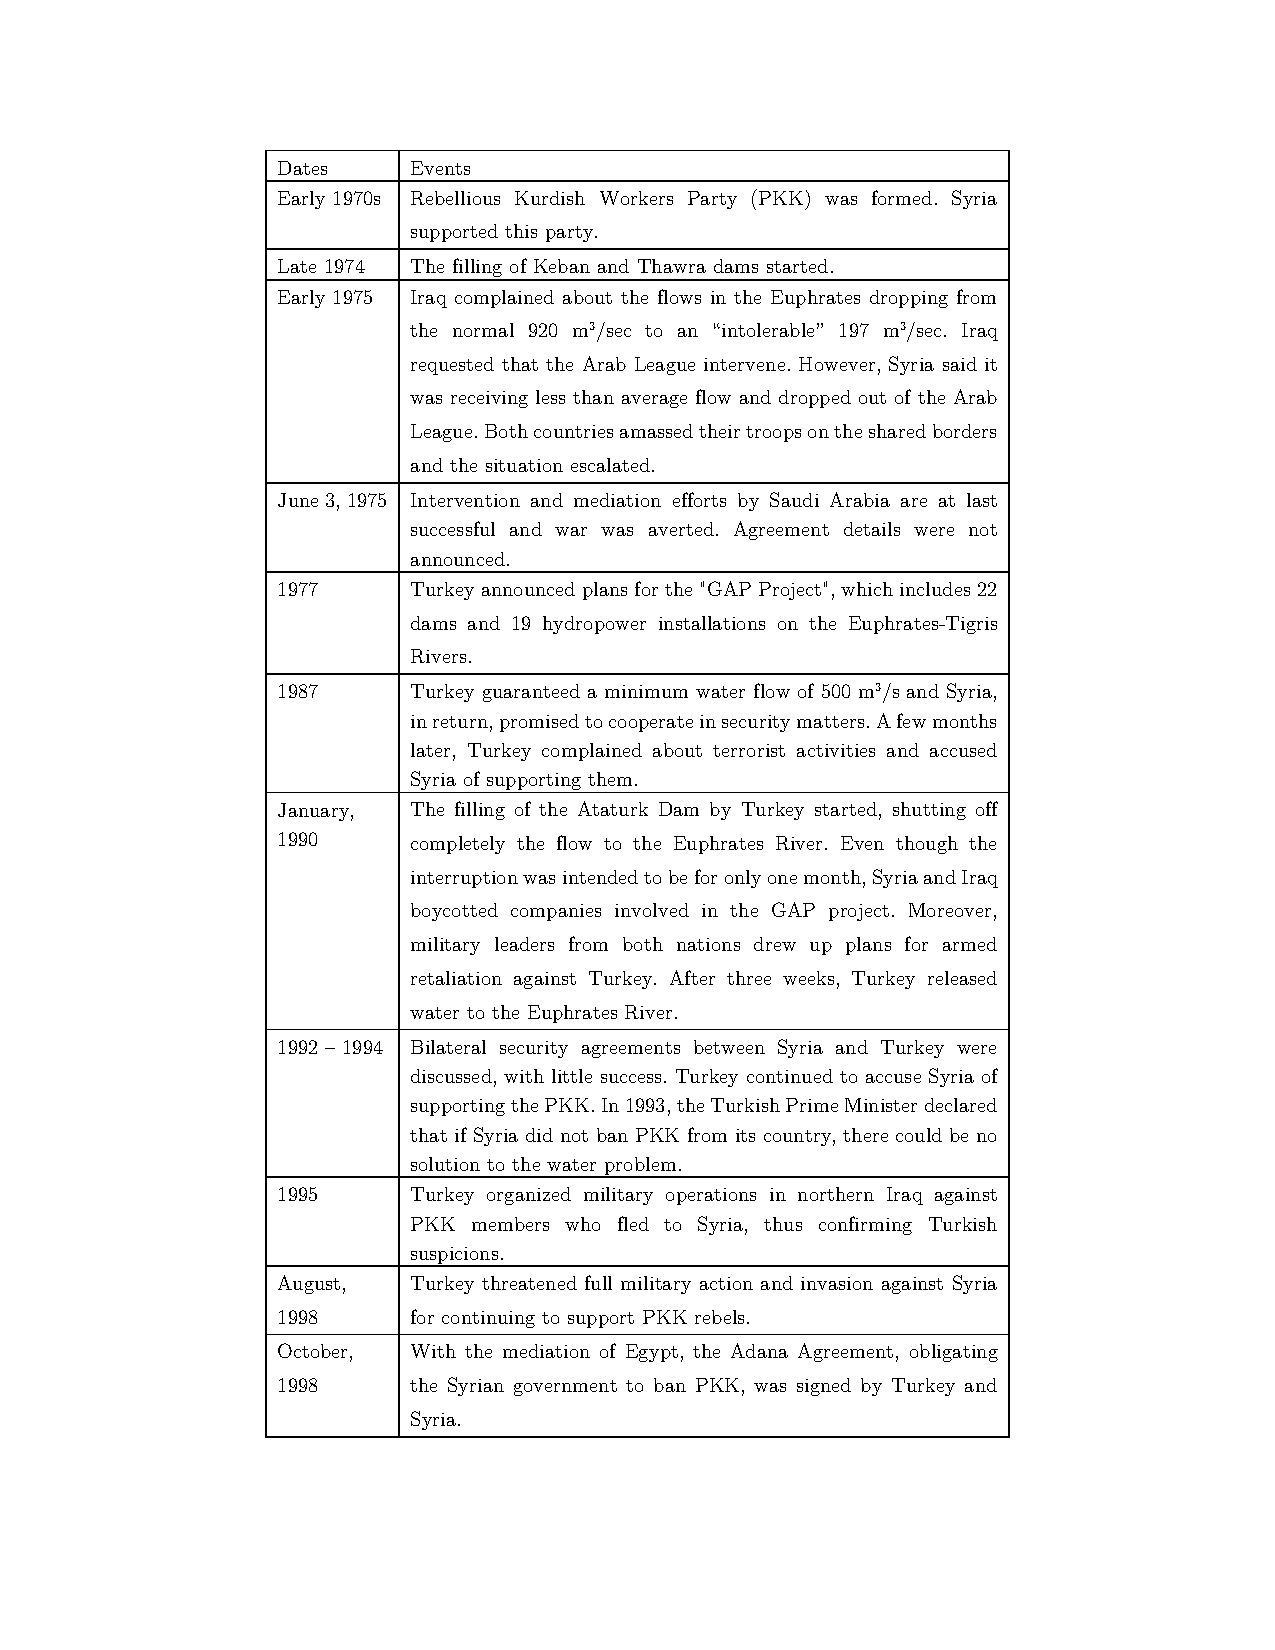
\includegraphics[scale=.88]{PDF-IMG/Euphrates_history.pdf}

\caption{Notable events related to conflicts along the Euphrates River}

\label{tbl:historyEuphrates}
\end{table}

%%%%%%%%%%%%%%%%%%%%%

\section{Conflict Analysis of the 1975 Dispute}
\label{Conflict1975Analysis}
The DMs and options for the 1975 conflict are given in Table \ref{tbl:t1}. Notice that Syria has an option regarding the release of the water plus an option of escalating the situation. Iraq has the single option of attacking Syria. Since both Saudi Arabia and the Soviet Union have similar preferences and reasons for getting involved, they are considered as a single DM labeled as ``Third Party". The Third Party has a single option of acting or not. Table \ref{tbl:t1} describes the options for each DM. Each option is labeled with a number and can be either taken (Y for yes) or not (N for no). For example, option 3, which is entitled Attack, is the situation in which Iraq can use military action to force Syria to release water into the Euphrates. Undertaking this option, as indicated by Y for yes, means using force, while not taking this option, N for no, indicates accepting the situation and allowing Syria to fill the Thawra Dam without escalation.

\begin{table}[H]
\centering
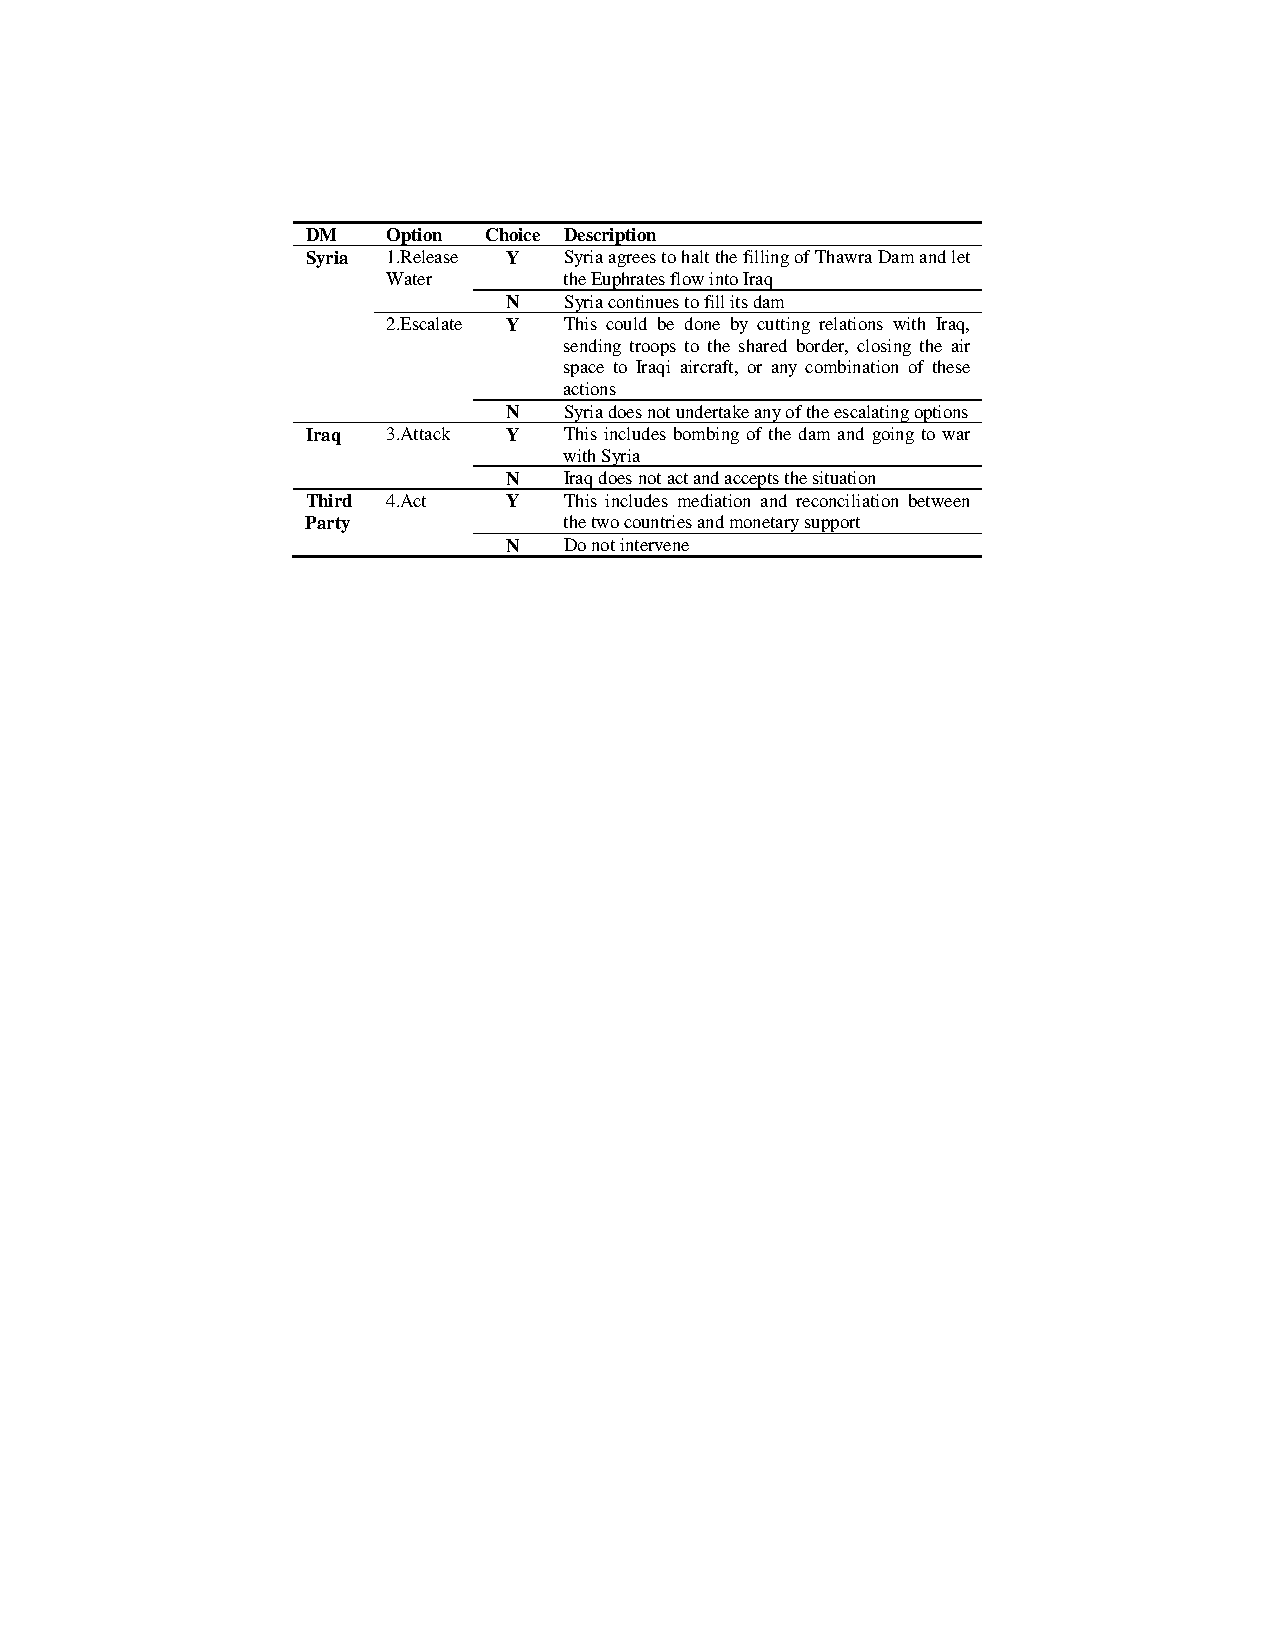
\includegraphics[scale=1]{PDF-IMG/tables/1.pdf}

\caption{DMs, options and descriptions for the 1975 conflict}

\label{tbl:t1}
\end{table}

To emphasize the effect of the third party, this conflict will be analyzed without and with the intervention of the third party. The sets of possible states are given in Tables \ref{tbl:t2} and \ref{tbl:t3}, respectively. Notice that there is one infeasible situation in which Syria both releases the water and escalates the situation at the same time (mutually exclusive options). Taking this into account resulted in the removal of two states in the model without the intervention of the third party and the removal of four states in the model with the participation of the third party.

\begin{table}[H]
\centering
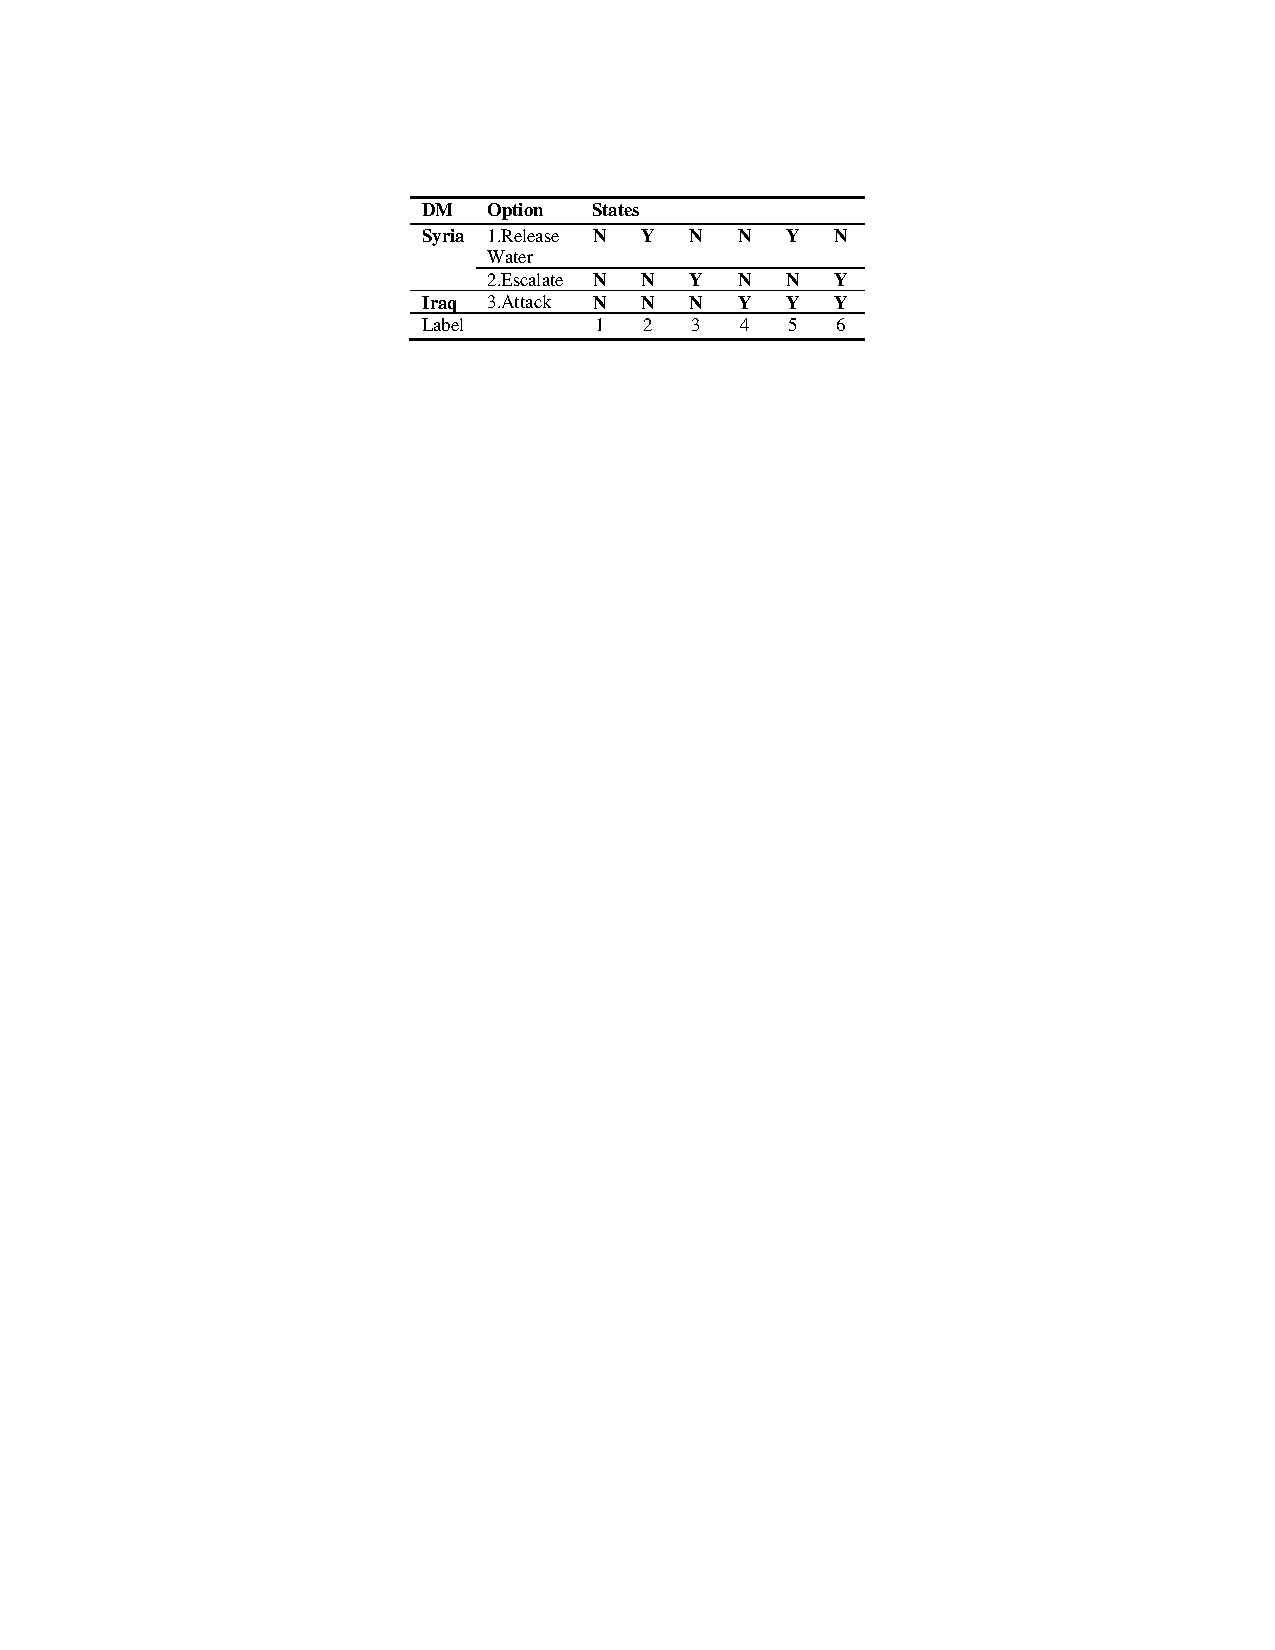
\includegraphics[scale=1]{PDF-IMG/tables/2.pdf}

\caption{DMs, options and states for the 1975 conflict without the third party}

\label{tbl:t2}
\end{table}

\begin{table}[H]
\centering
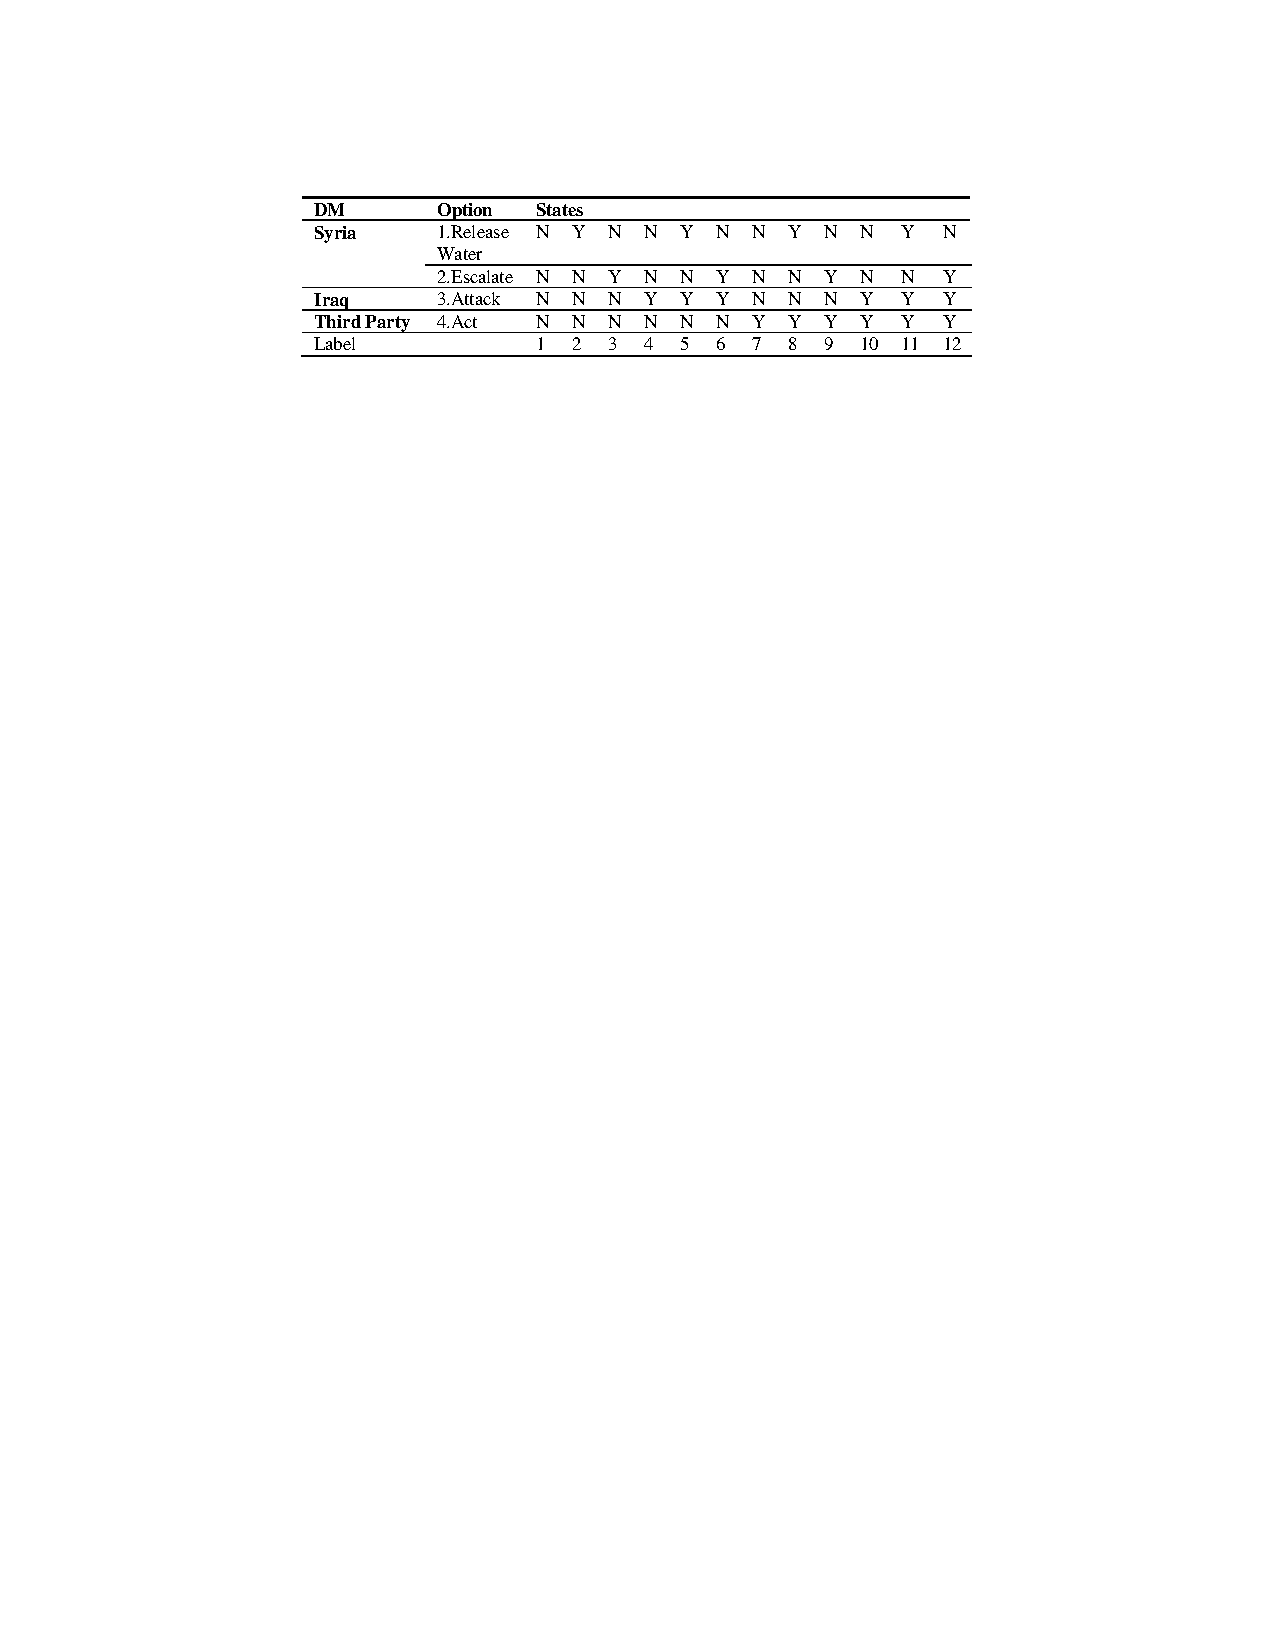
\includegraphics[scale=1]{PDF-IMG/tables/3.pdf}

\caption{DMs, options and states for the 1975 conflict with the third party}

\label{tbl:t3}
\end{table}

Figures \ref{fig:IrSyGM} and \ref{fig:IrSyGM2} show the integrated Graph Model of the conflict both without and with the participation of the third party, respectively. The numbers in the nodes refer to the state numbers as indicated in Tables \ref{tbl:t2} and \ref{tbl:t3}. The lines with arrows between the nodes are moves that can be carried out by the indicated DM in one step. 

\begin{center}
\begin{figure}[H]
\centering
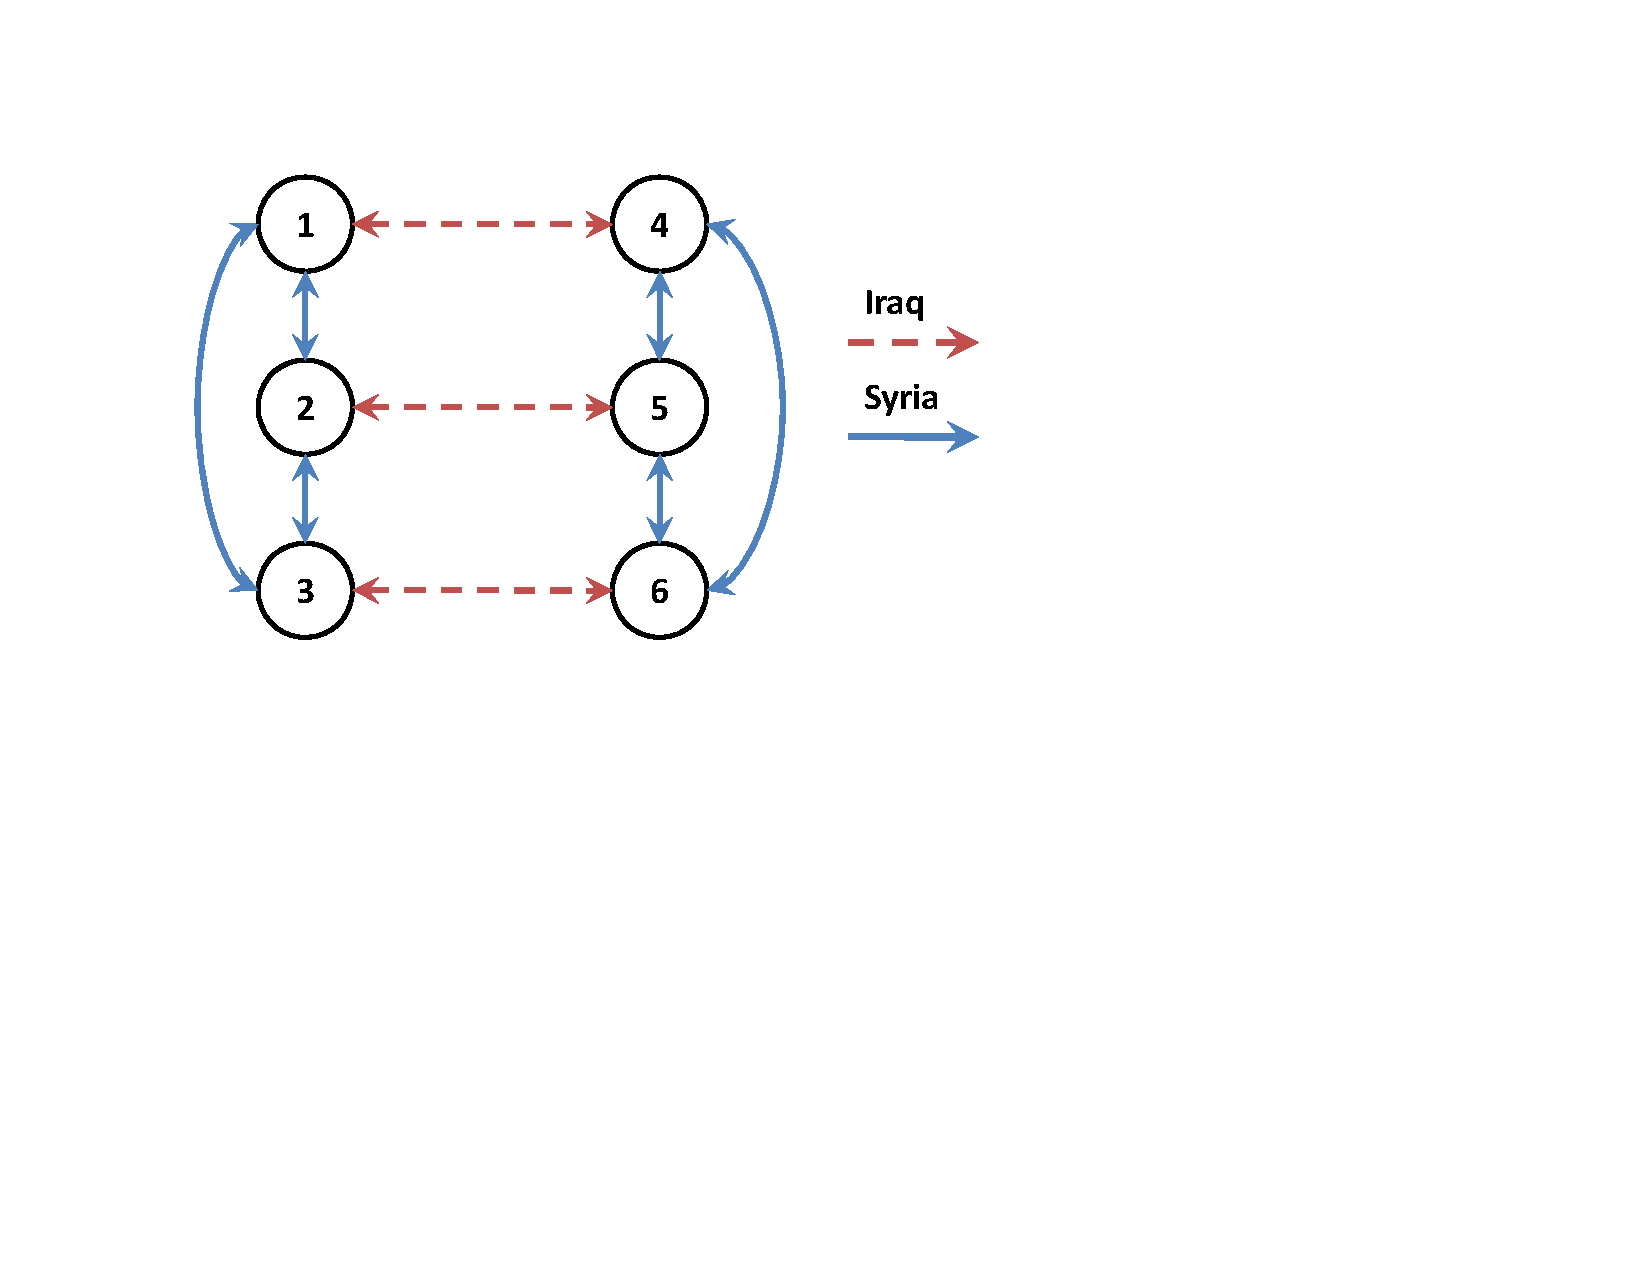
\includegraphics[scale=0.6]{PDF-IMG/IrSy1.pdf}

\caption{Integrated Graph Model of the 1975 conflict without the third party}

\label{fig:IrSyGM}
\end{figure}
\end{center}

\begin{center}
\begin{figure}[H]
\centering
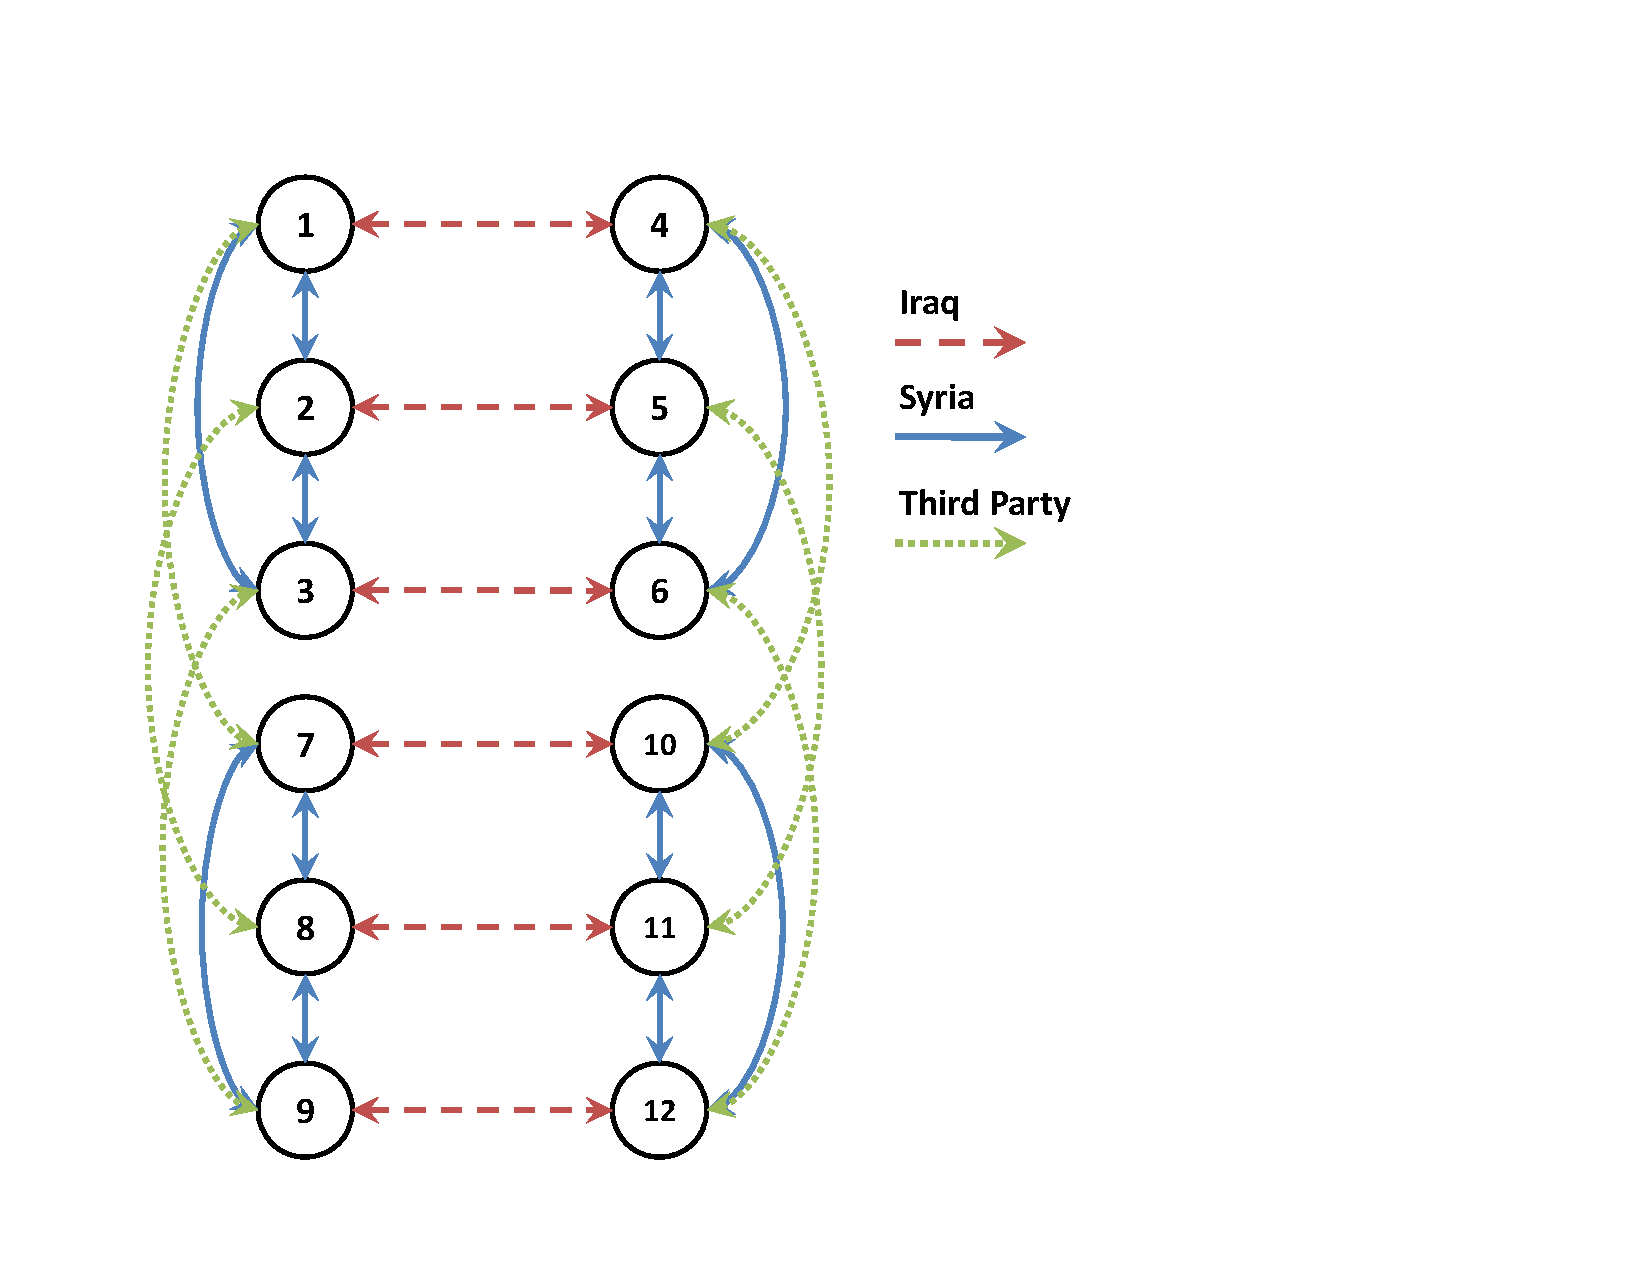
\includegraphics[scale=0.5]{PDF-IMG/IrSy2.pdf}

\caption{Integrated Graph Model of the 1975 conflict with the third party}

\label{fig:IrSyGM2}
\end{figure}
\end{center}

Table \ref{tbl:t4} presents the preference prioritization information for each DM in the 1975 conflict without the participation of the third party, from most important at the top to least important at the bottom for each DM. The statements presented herein are a sample of how the ranking of states is constructed. This information is used to order the states from most to least preferred by the DM. Assuming transitivity for the preferences, Table \ref{tbl:t5} presents the ranking of states from most to least preferred for both Syria and Iraq using option prioritization \citep{hipel1997decision,fang2003a,fang2003b}. For example, State 1, which is the status quo, is the best state to be in for Syria. State 5, in which Syria releases the Euphrates and Iraq attacks at the same time, is considered the worst possible state for Syria.

\begin{table}[H]
\centering
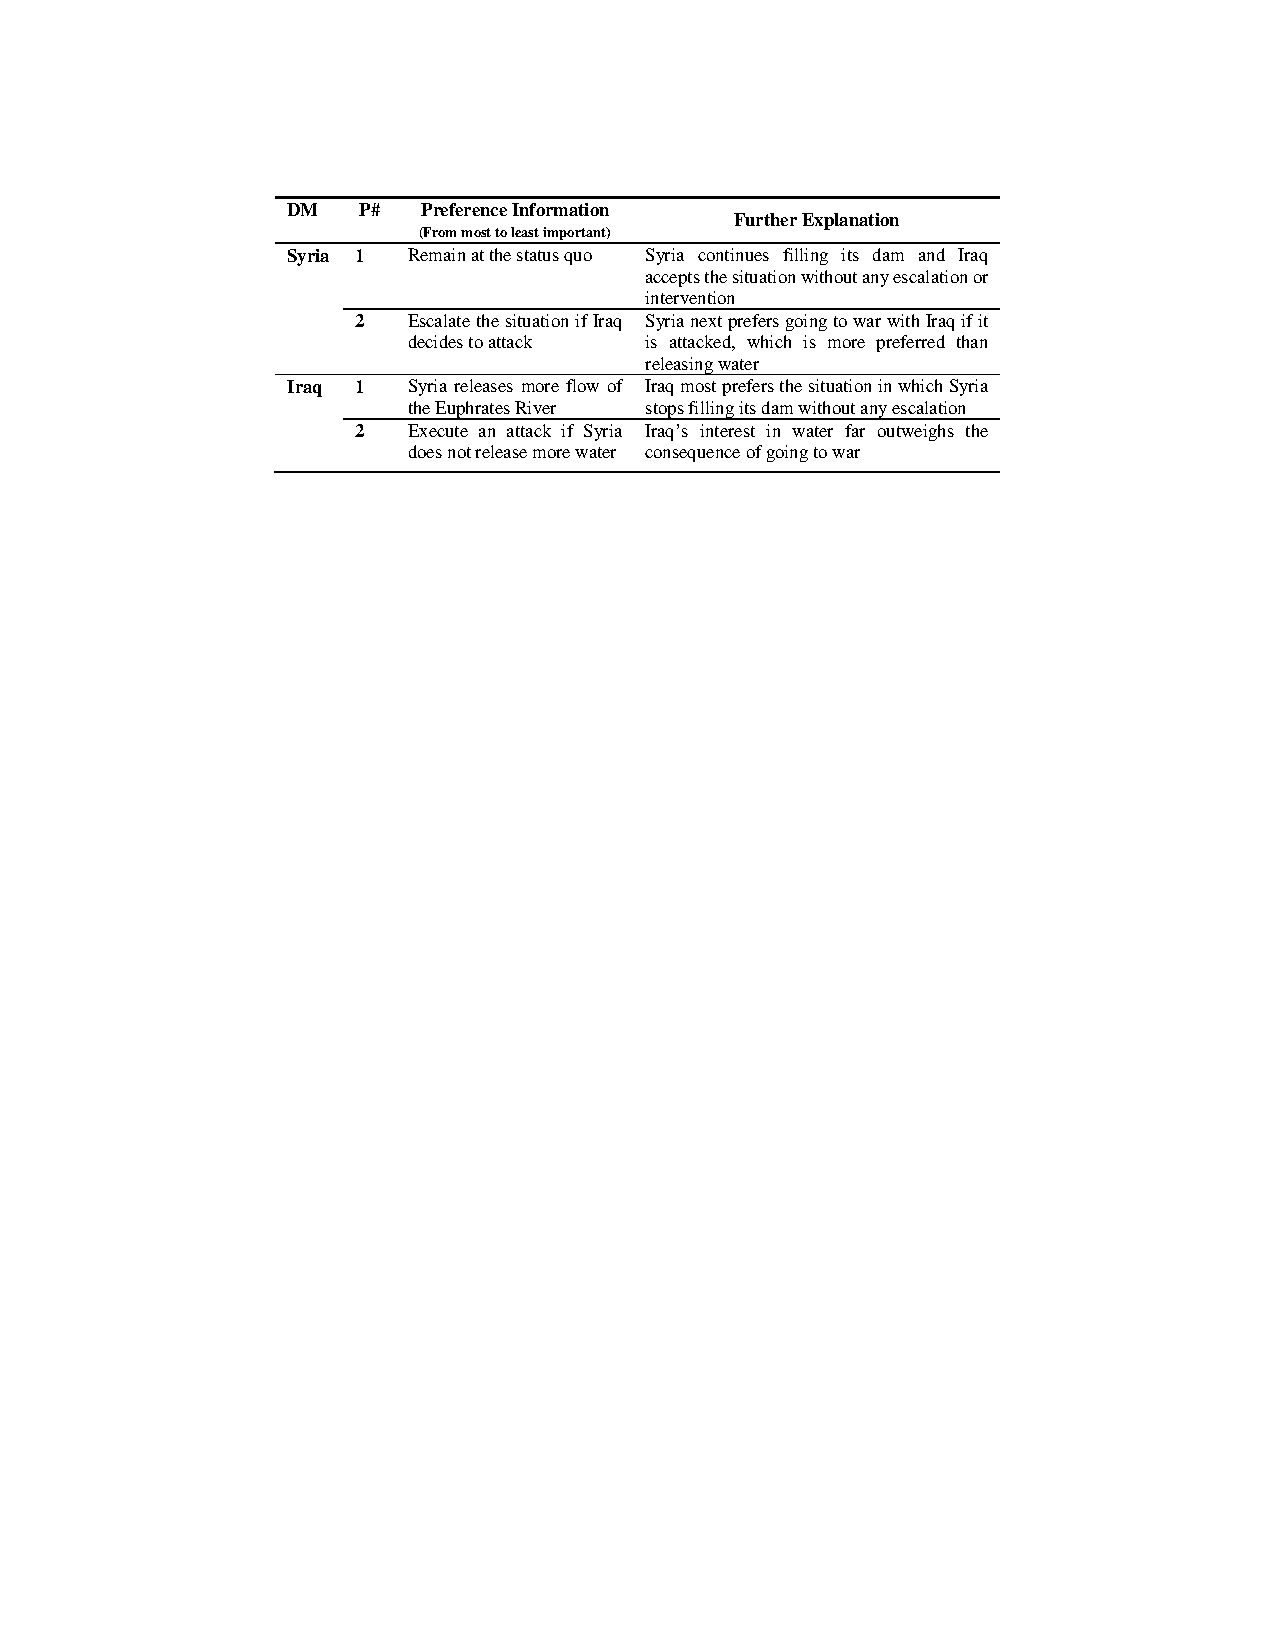
\includegraphics[scale=1]{PDF-IMG/tables/4.pdf}

\caption{Preference prioritization information for the 1975 conflict without the third party}

\label{tbl:t4}
\end{table}


\begin{table}[H]
\centering
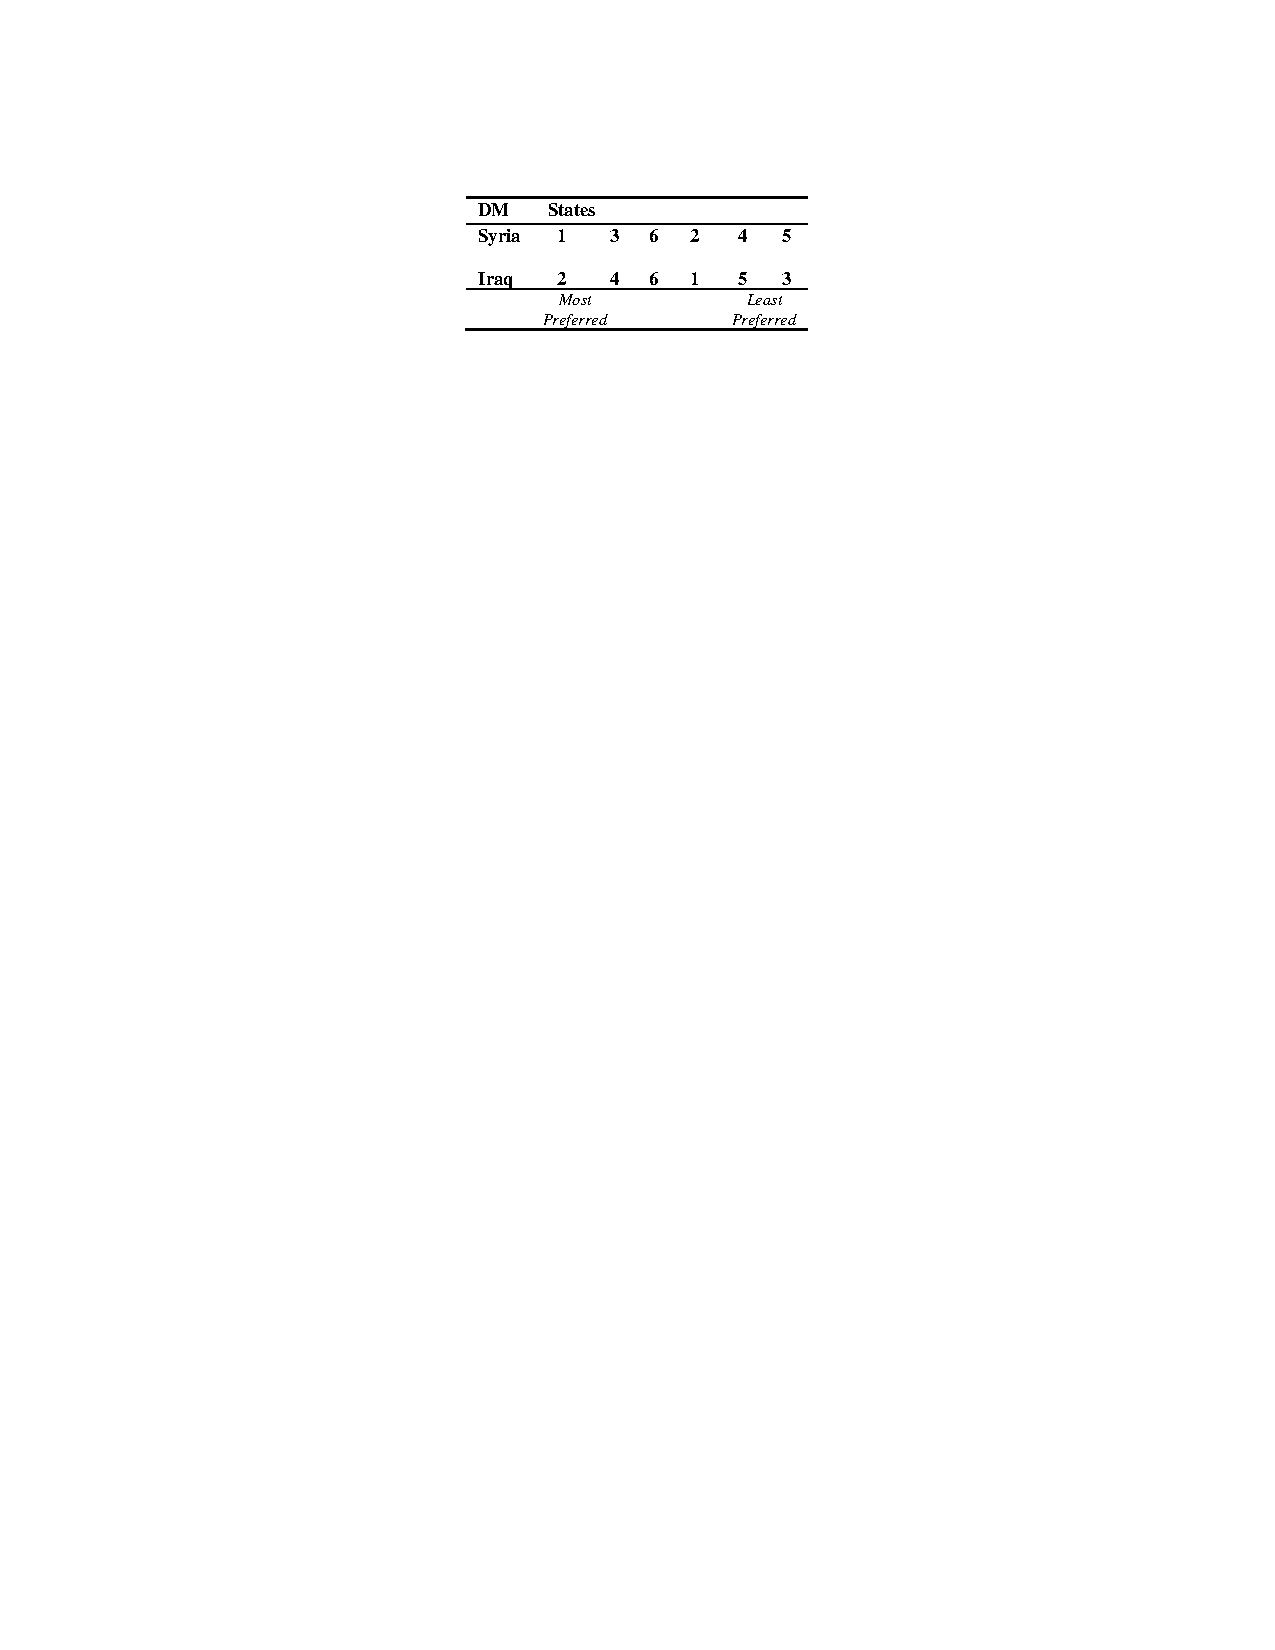
\includegraphics[scale=1]{PDF-IMG/tables/5.pdf}

\caption{Ranking of states for the DMs in the 1975 conflict without the third party}

\label{tbl:t5}
\end{table}

The third party could be viewed as an actual DM if it has its own options and preferences. However, if the party is not an actual stakeholder in the conflict but is motivated to bring about a more preferred equilibrium, then it can be categorized as Arbitrator, Coordinator or Donor \citep{sakamoto2005}. If the party has the influence to change other DMs' preferences or options, then the party is called a Donor. On the other hand, if the party has the power to exclude some states, then it is considered to be an Arbitrator. In this conflict, the third party, Saudi Arabia, is clearly a Donor as it contributed to financing the basin development and both DMs, Syria and Iraq, want to please Saudi Arabia. Therefore, DMs' preferences, especially on the part of Syria, are changed. Table \ref{tbl:t6} presents the preference prioritization information for each DM in the 1975 conflict with the participation of the third party from most to least preferred. Table \ref{tbl:t7} gives the preferences for Syria, Iraq, and the third party from most to least preferred.

\begin{table}[H]
\centering
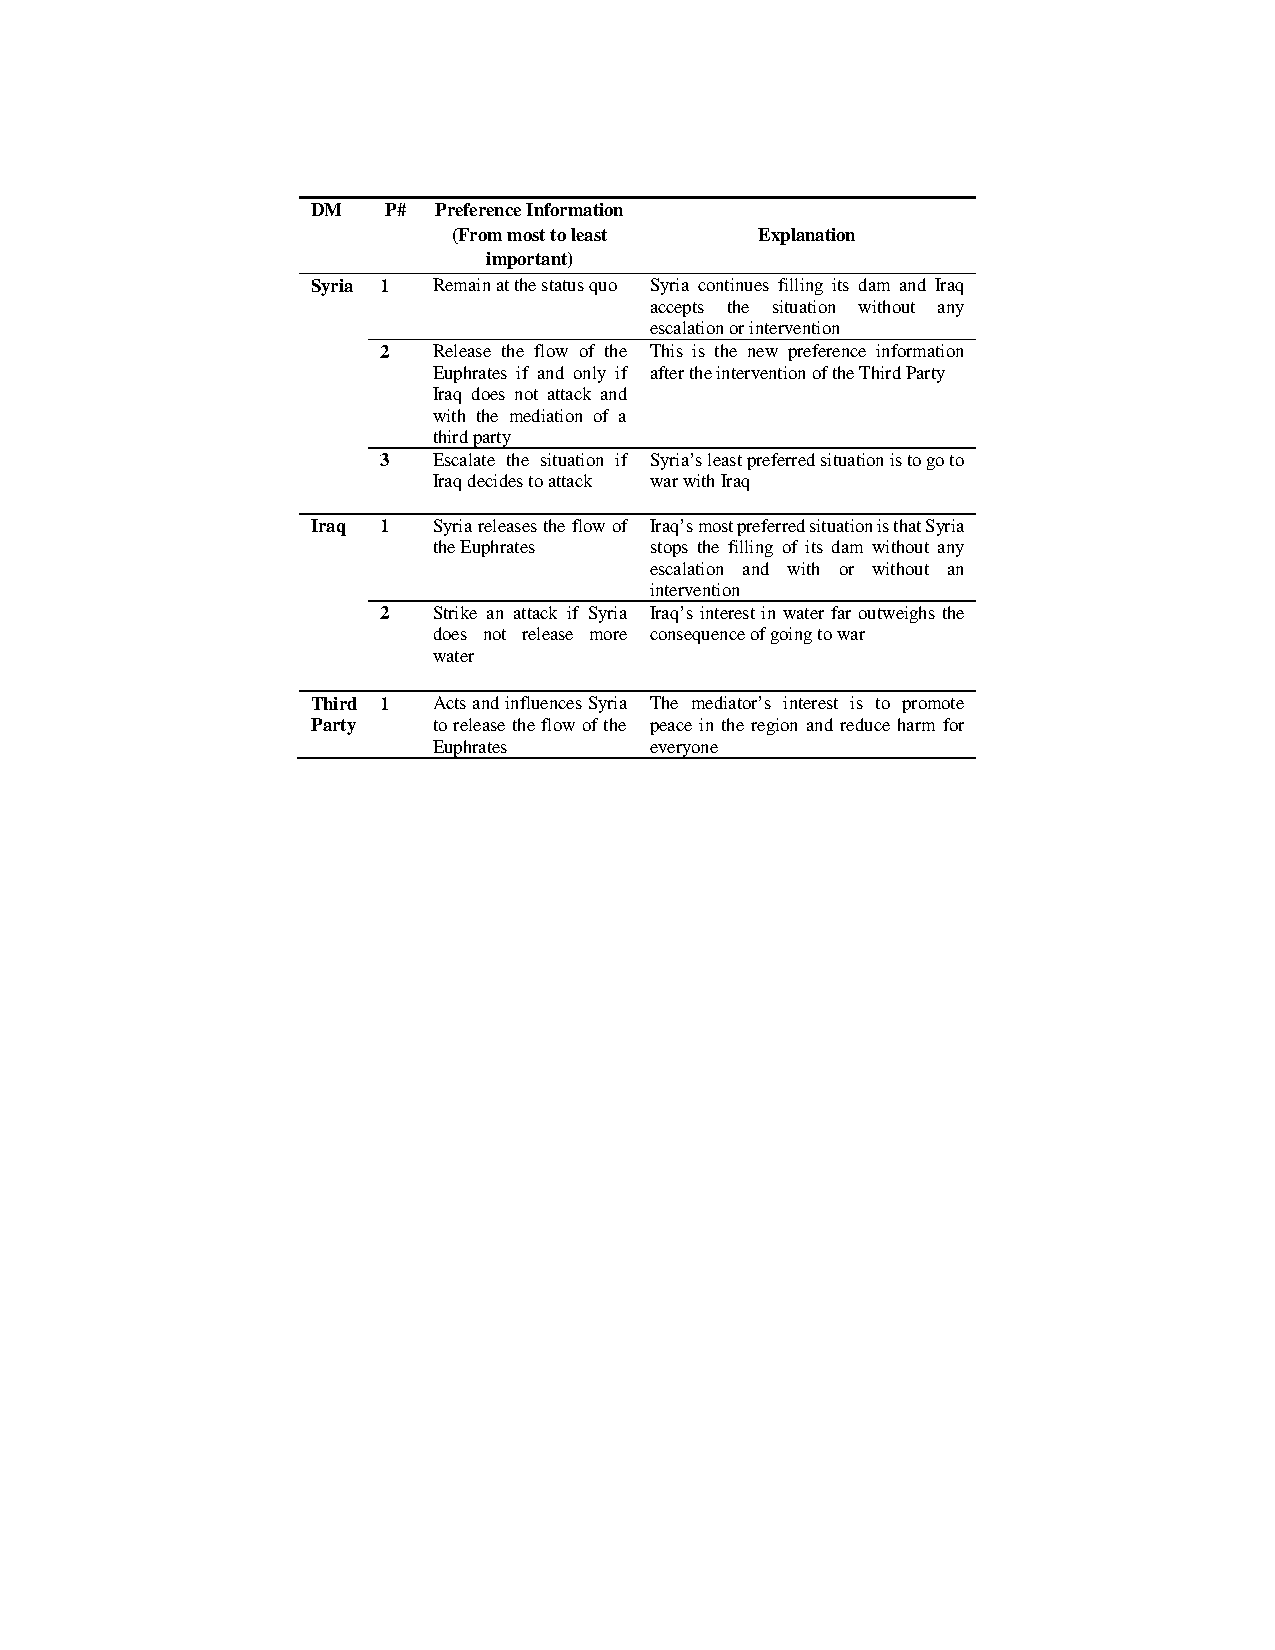
\includegraphics[scale=1]{PDF-IMG/tables/6.pdf}

\caption{Preference prioritization information for the 1975 conflict with the third party}

\label{tbl:t6}
\end{table}

\begin{table}[H]
\centering
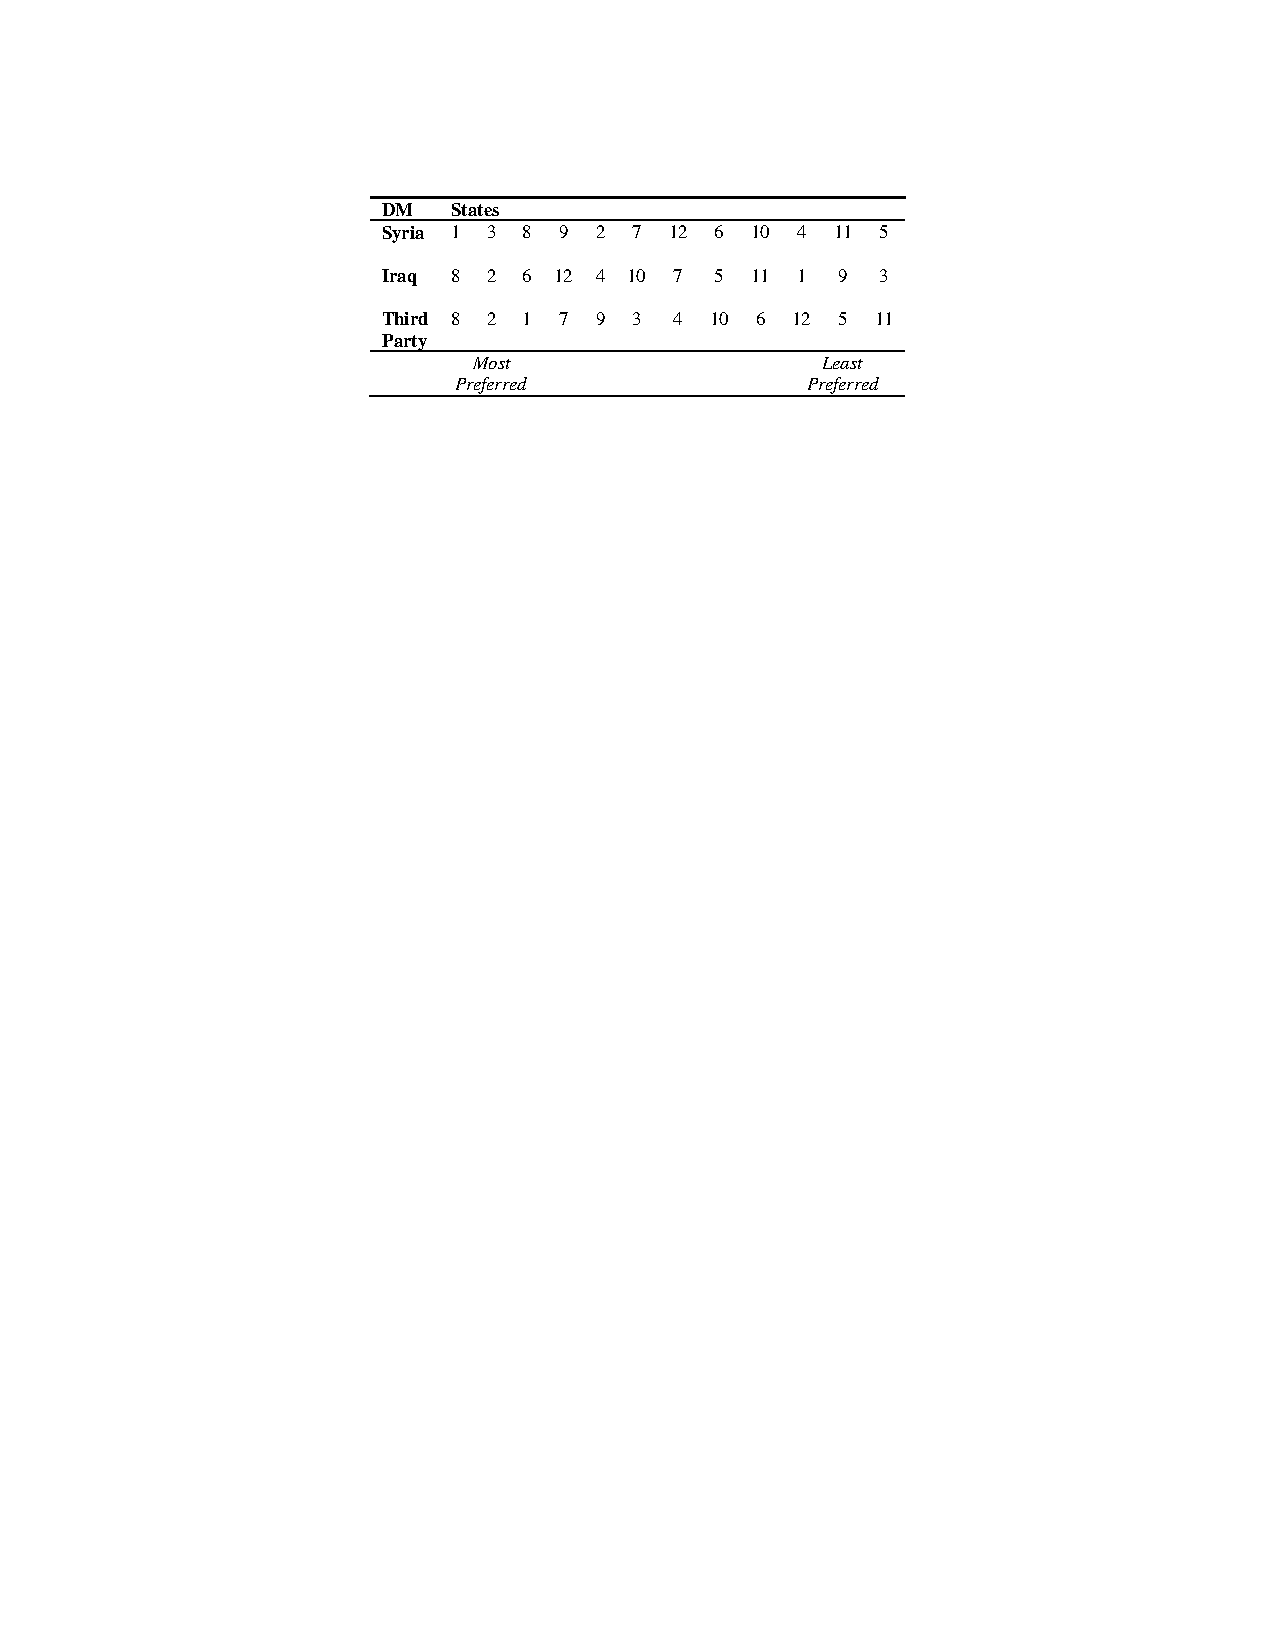
\includegraphics[scale=1]{PDF-IMG/tables/7.pdf}

\caption{Ranking of states for the DMs in the 1975 conflict with the third party}

\label{tbl:t7}
\end{table}

The objective of the analysis is to determine the equilibrium states, which are the states from which no DM is motivated to move and, therefore, the conflict will probably end at that particular state. To determine the equilibrium states we use stability definitions (or solution concepts), which describe human behavior and patterns based on moves and counter moves. Equilibria are states that are stable for all DMs. After inputting the foregoing information into the decision support system GMCR II, equilibrium results are obtained for both Syria and Iraq without the third party (Table \ref{tbl:t8}) and with the third party (Table \ref{tbl:t9}). Restricting Iraq's alternative of attacking does not affect the equilibria for both cases. In Tables \ref{tbl:t8} and \ref{tbl:t9}, the left column gives the different stability definitions while the remaining columns present the stability calculation results for each solution concept corresponding to the state. Nash and Sequential Stability (SEQ) are considered the strongest stability definitions. General Metarationality (GMR) and Symmetric Metarationality (SMR) are not considered as strong stability definitions since DMs are permitted to harm themselves during the process of sanctioning. \citet{Fang1989} discuss the relationships among the different solution concepts.

\begin{table}[H]
\centering
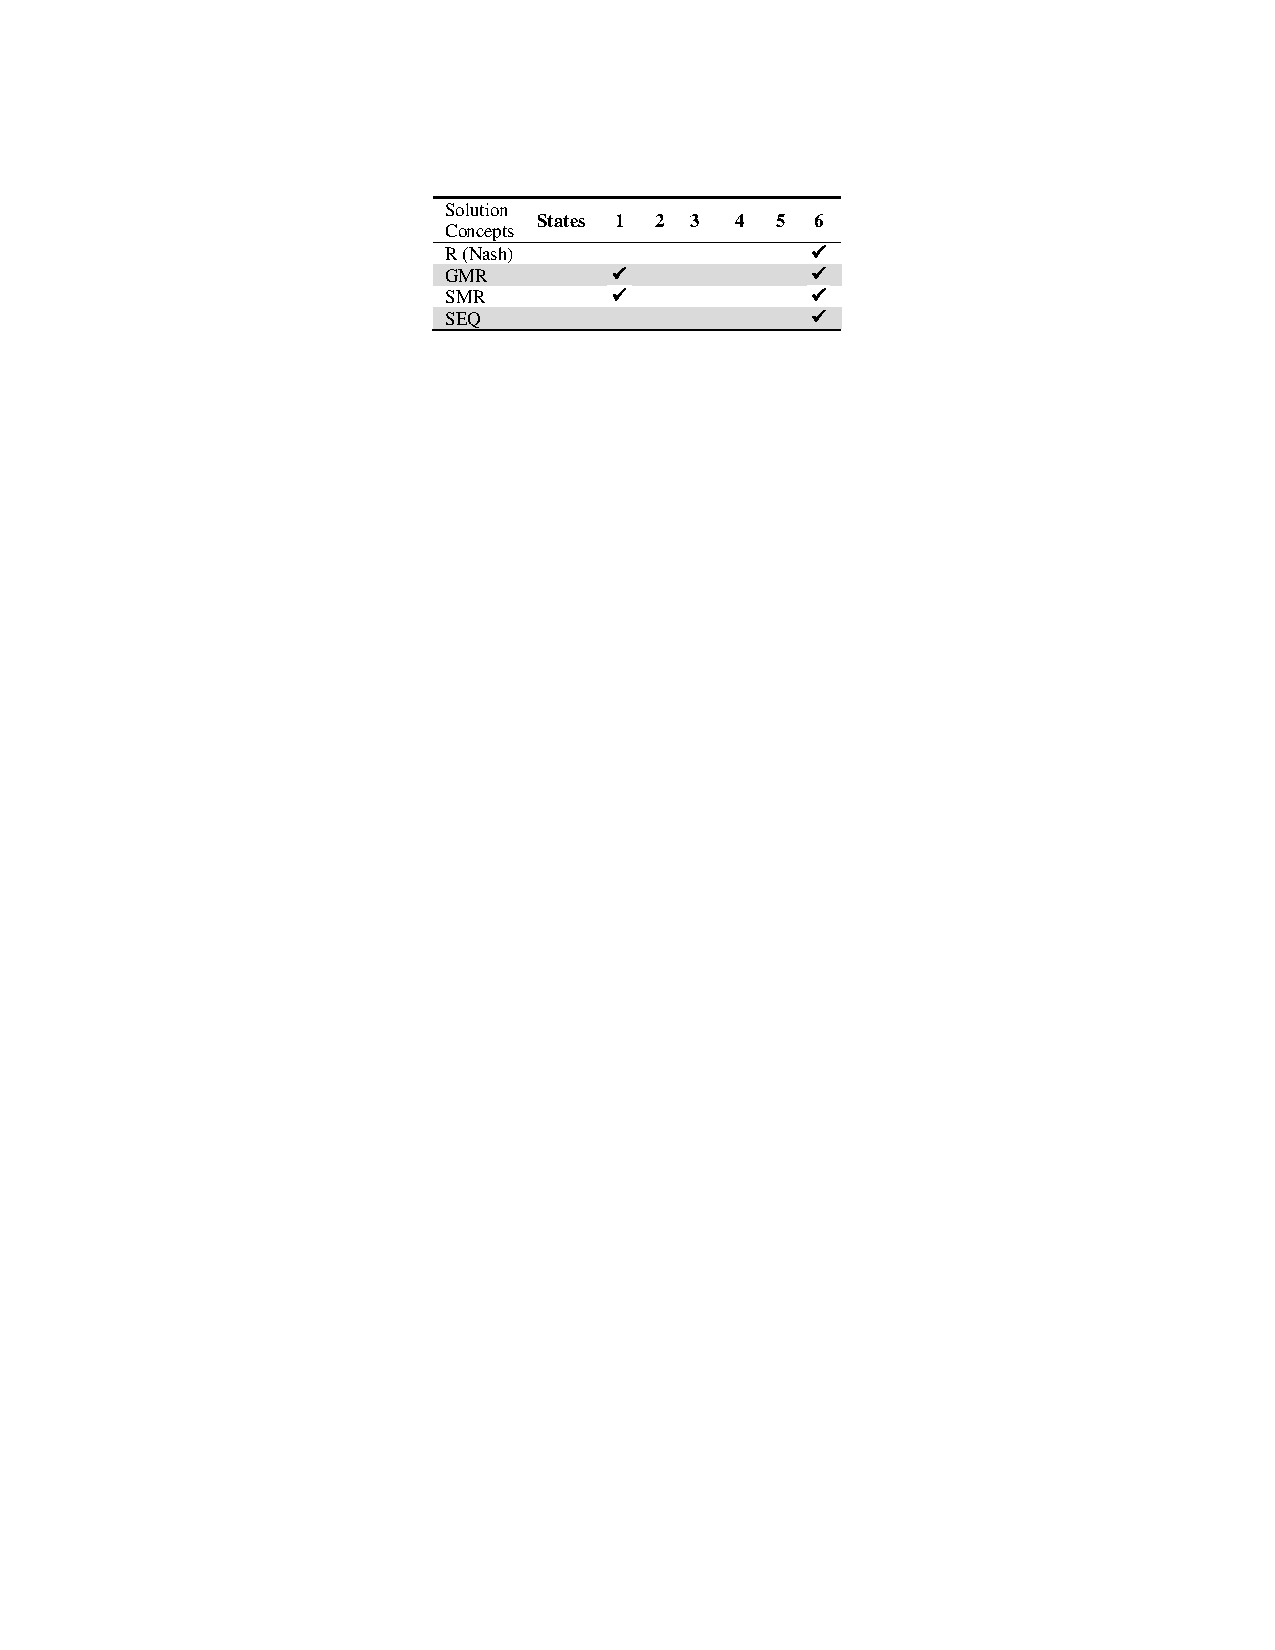
\includegraphics[scale=1]{PDF-IMG/tables/8.pdf}

\caption{Equilibrium results for the 1975 conflict without the third party}

\label{tbl:t8}
\end{table}

\begin{table}[H]
\centering
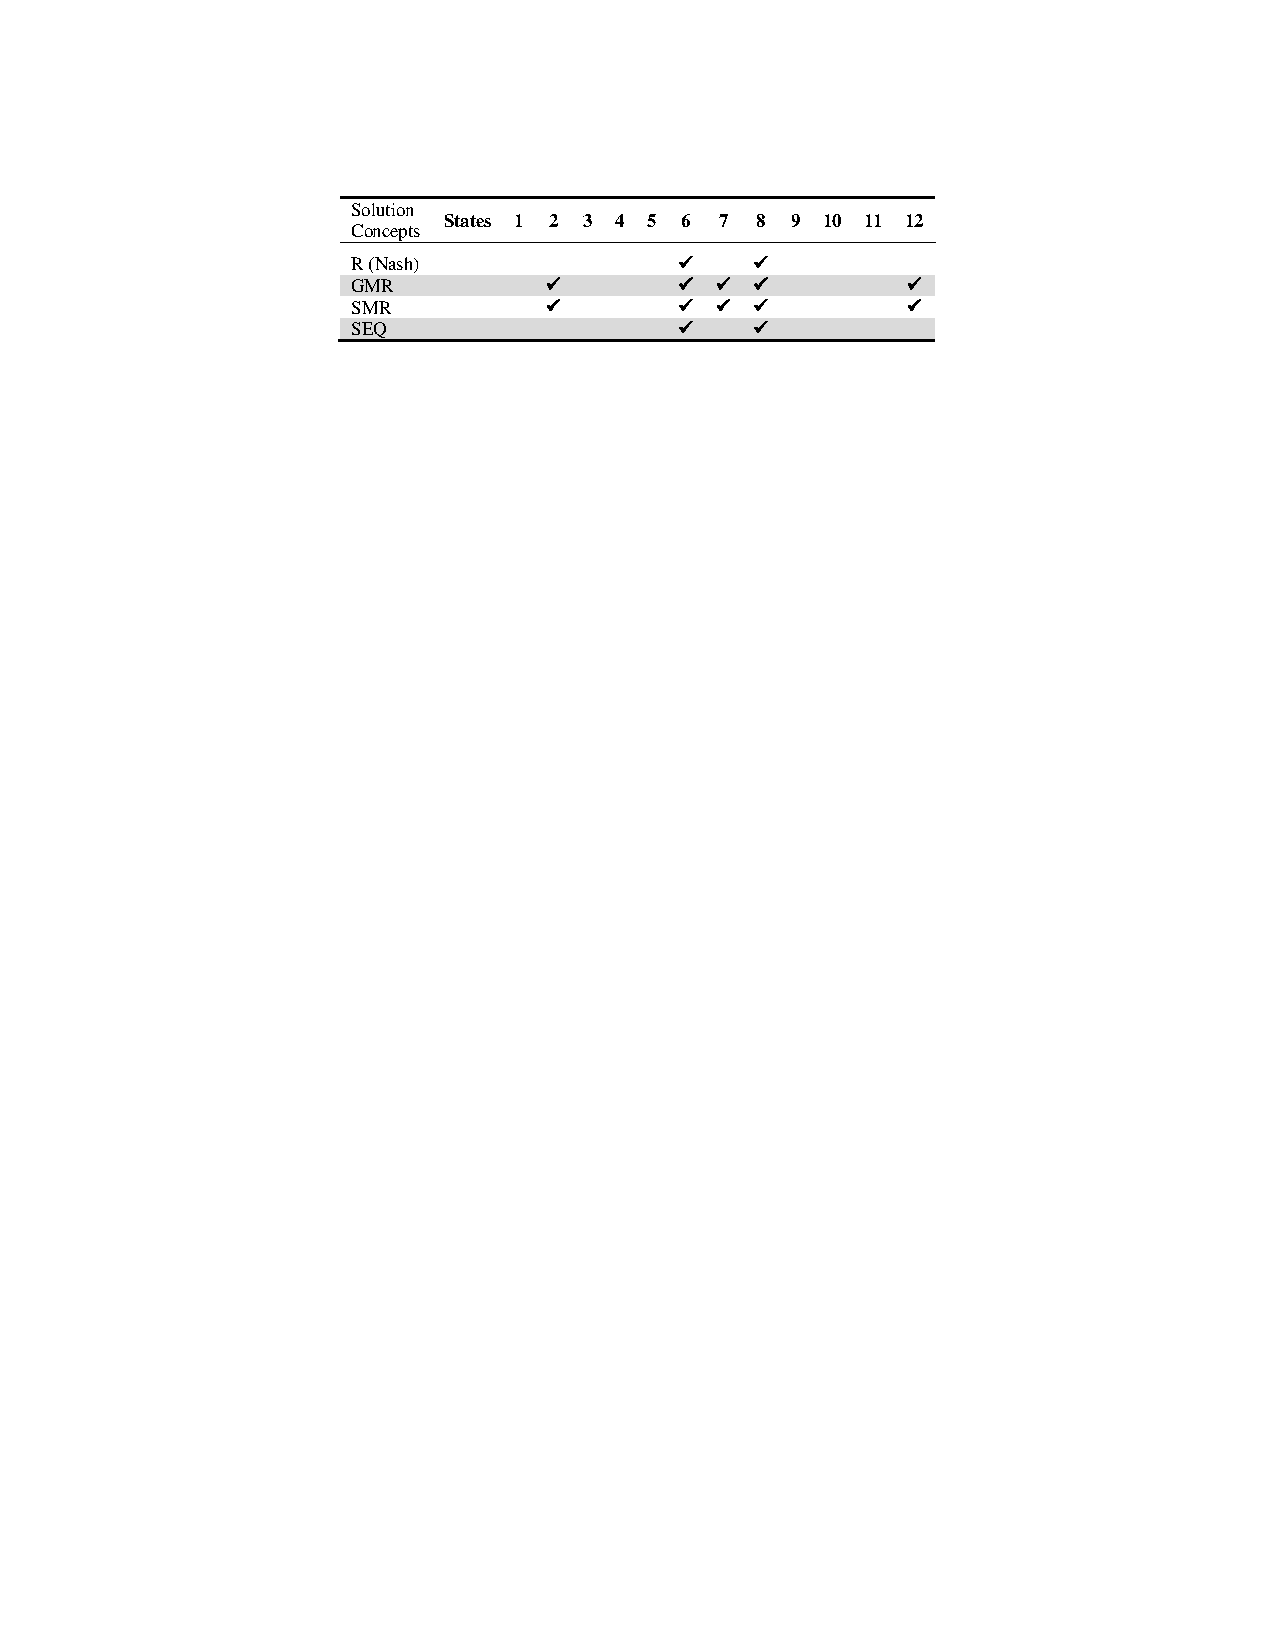
\includegraphics[scale=1]{PDF-IMG/tables/9.pdf}

\caption{Equilibrium results for the 1975 conflict with the third party}

\label{tbl:t9}
\end{table}

It is clear from the aforementioned analysis that when the third party does not participate (Table  \ref{tbl:t8}), the strongest equilibrium is state 6 which means that both Syria and Iraq go to war. And that is what nearly happened as both countries amassed their troops on their shared border. The status quo, State 1, is a very weak equilibrium and the unilateral improvement by Iraq will most likely be taken; that is, Iraq will move to state 4 in which it will attack. In contrast, with the intervention of the third party, a new equilibrium is introduced: State 8 in which Syria releases water and no escalation or attack from Iraq occurs. Referring to the ranking of states in Tables  \ref{tbl:t5} and  \ref{tbl:t7} as well as the integrated graphs in Figures \ref{fig:IrSyGM} and \ref{fig:IrSyGM2}, one can easily view the unilateral moves and improvements for each DM. A unilateral move is any possible move controlled by that particular DM, whereas a unilateral improvement necessitates that this move is also a movement to a more preferred state.  
The analysis of the conflict demonstrates how each DM's preferences may have an impact on the overall conflict. Table \ref{tbl:t10} provides the actual historical evolution of the conflict when moving from the status quo on the left via several intermediate states to the final equilibrium on the right. One can clearly see how both Syria and Iraq almost went to war until the third party intervened. It is clear that the actual historical evolution of the conflict is consistent with the earlier analysis.


\begin{table}[H]
\centering
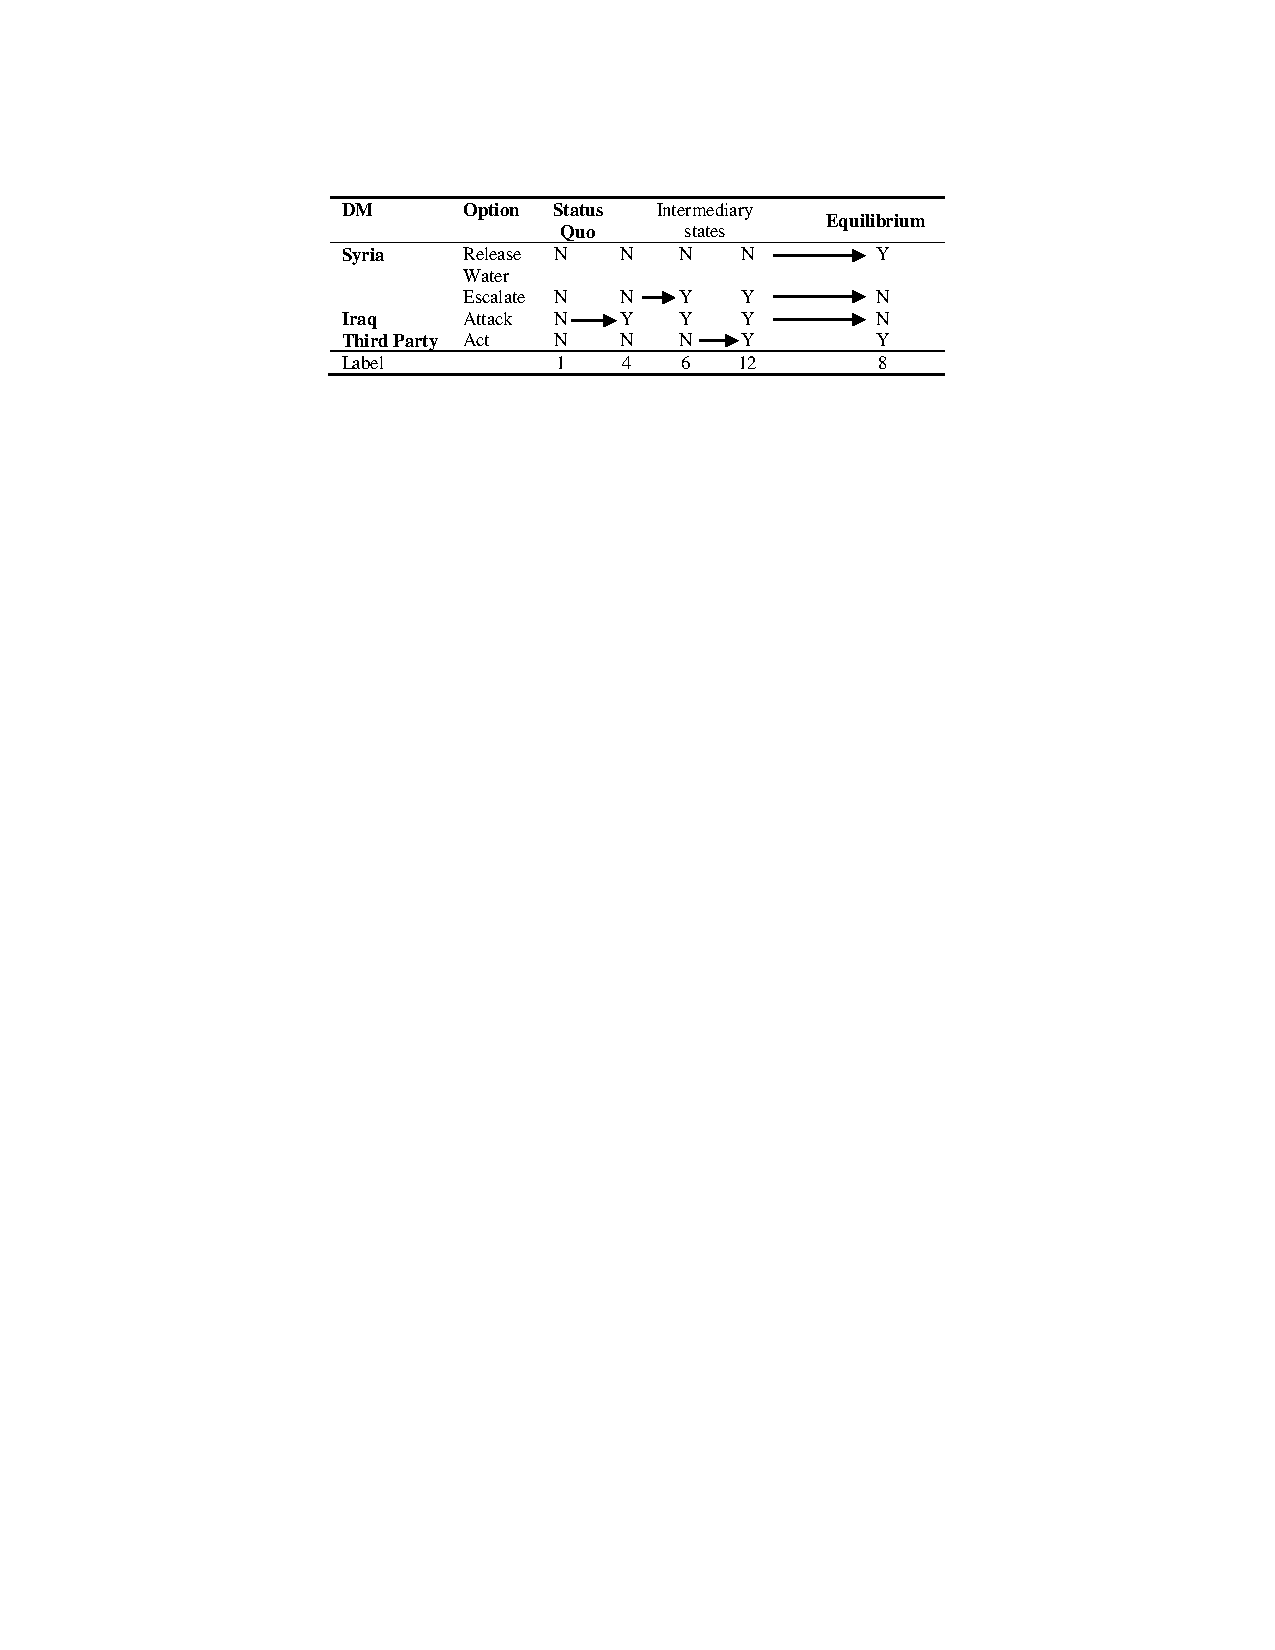
\includegraphics[scale=1]{PDF-IMG/tables/10.pdf}

\caption{Historical evolution of the 1975 conflict}

\label{tbl:t10}
\end{table}
% % % % % % % % % % % % % % % % % % % % %

\section{Strategic Study of the 1990 Conflict}
\subsection{Modeling and analysis}
The DMs and options for the 1990 conflict are given in Table \ref{tbl:Tables1990T12}. Turkey has two options: escalate the dispute with Syria and/or decrease the flow of the Euphrates. Syria possesses the two options of stopping its support for the PKK or escalating the situation. Iraq controls the single option of escalating the situation against Turkey.


\begin{table}[H]
\centering
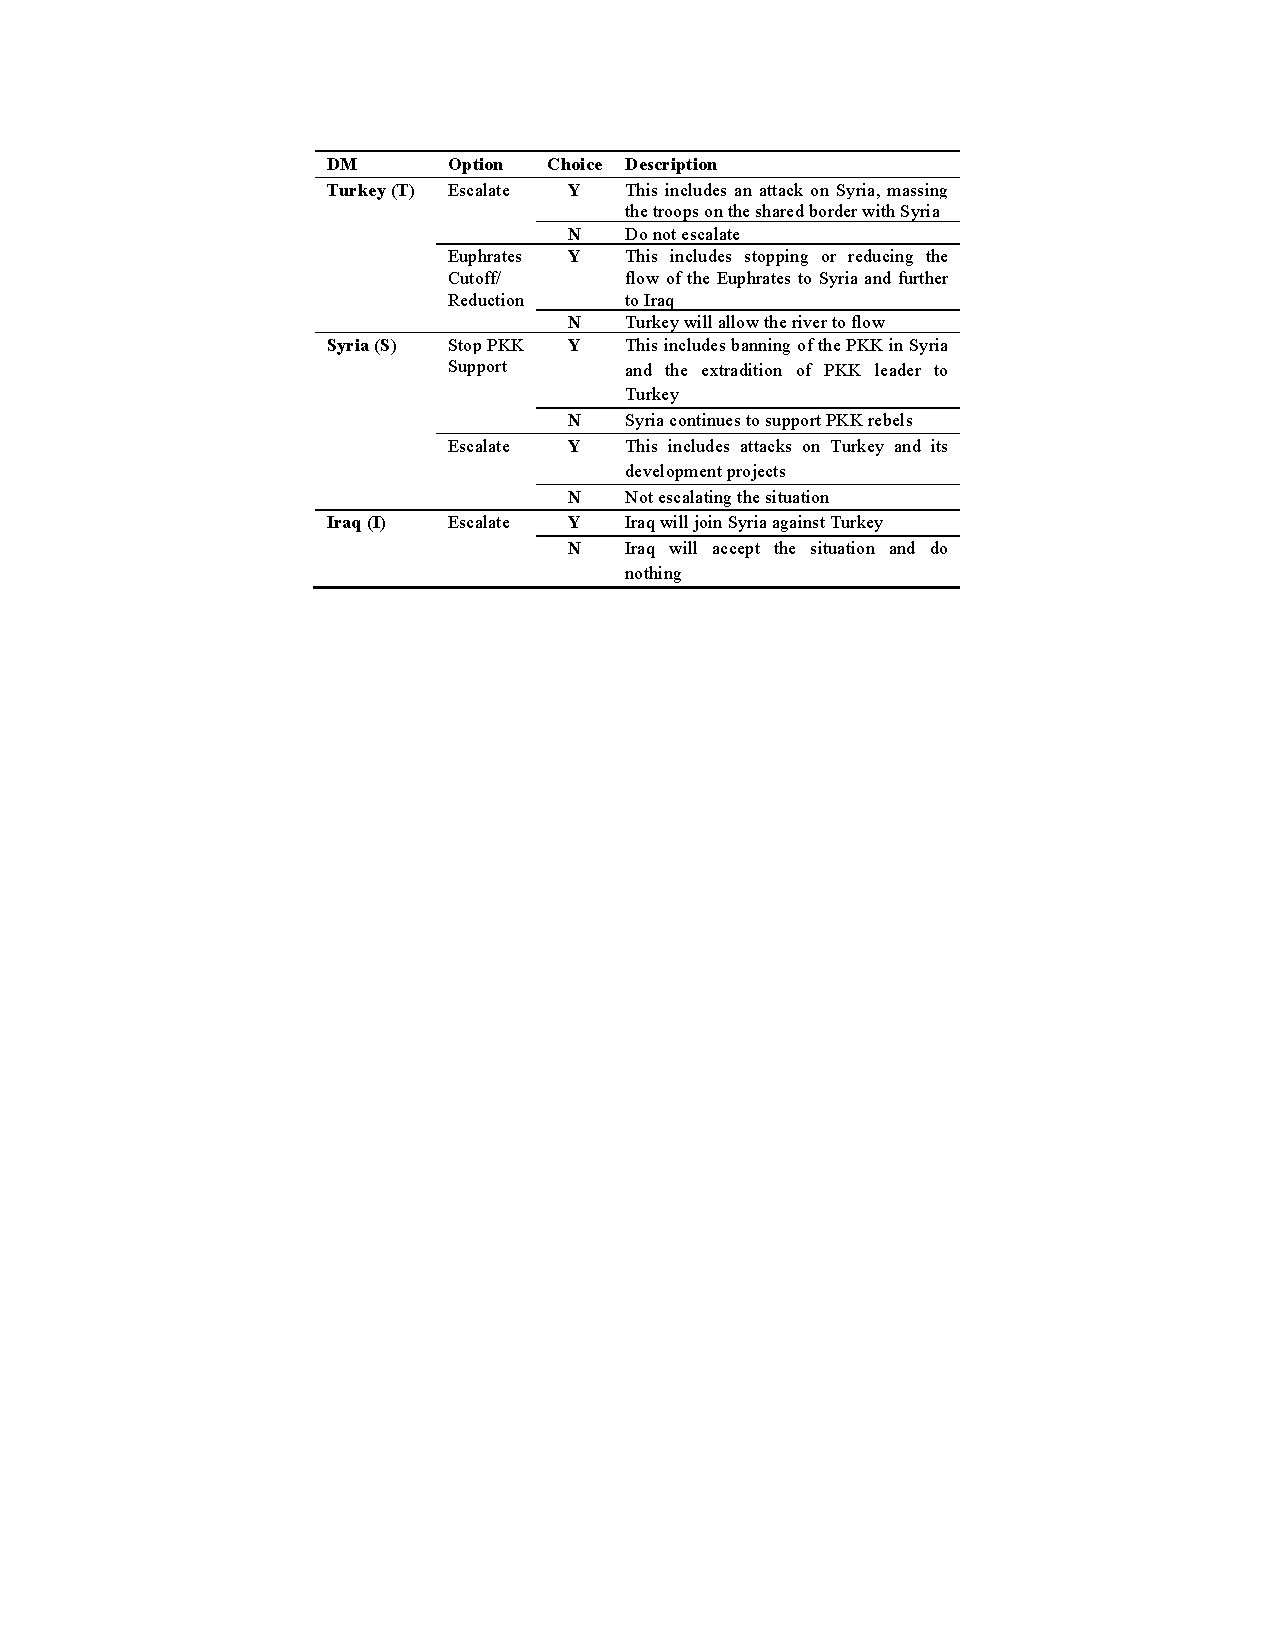
\includegraphics[scale=1]{PDF-IMG/tables/Tables1990T12.pdf}

\caption{DMs, options and description for the 1990 conflict}

\label{tbl:Tables1990T12}
\end{table}

The set of possible feasible states is given in Table \ref{tbl:Tables1990T13}. Notice that the number of mathematically possible states equals $2^5$ = 32 since there are 5 options each of which can be taken or not. However, Syria cannot both ban PKK and escalate at the same time (mutually exclusive options) and there is no point for Iraq to escalate if Turkey does not cut the water and Syria does not escalate. Removing the foregoing infeasible situations leads to a total of 20 feasible states or scenarios.


\begin{table}[H]
\centering
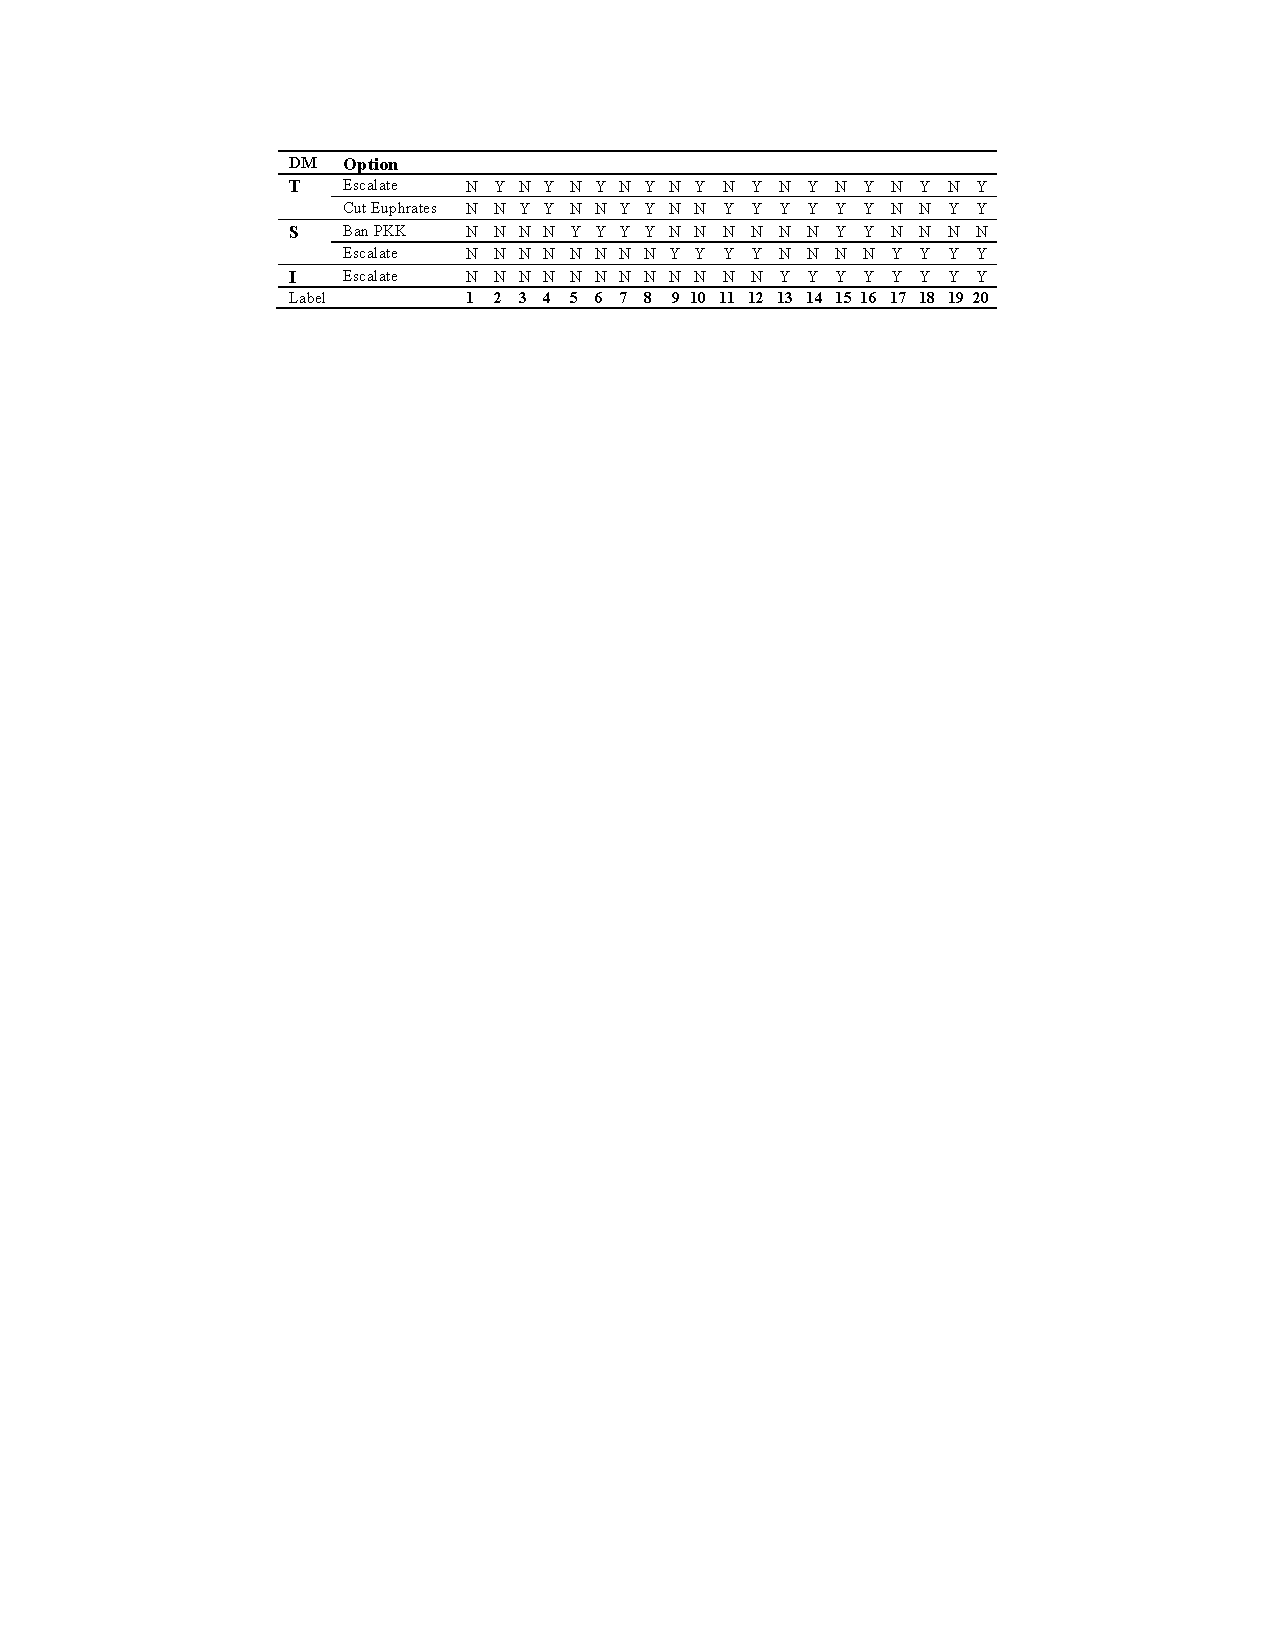
\includegraphics[scale=1]{PDF-IMG/tables/Tables1990T13.pdf}

\caption{DMs, options and states for the 1990 conflict}

\label{tbl:Tables1990T13}
\end{table}

This conflict is now analyzed using a regular analysis and an in-depth coalition analysis based on the procedure described by \citet{kilgour2001coalition} and \citet{inohara2008a,inohara2008b}. Figure \ref{fig:FIG4} illustrates the possible moves by Turkey. Figure \ref{fig:FIG5} shows the Integrated Graph Model of the conflict and possible moves by each of Syria and Iraq unilaterally. Figure \ref{fig:FIG6} displays the Coalition Graph Model of the conflict for both DMs, Syria and Iraq. Coalition improvements are denoted in this graph by a filled-in circle while coalition moves are denoted by a normal arrow. For example, from state 18 (top right corner) in Figure \ref{fig:FIG6}, there is a coalition move to states 2 and 10. However, the coalition move to state 10 is a coalition improvement by both Syria and Iraq. 

\begin{center}
\begin{figure}[H]
\centering
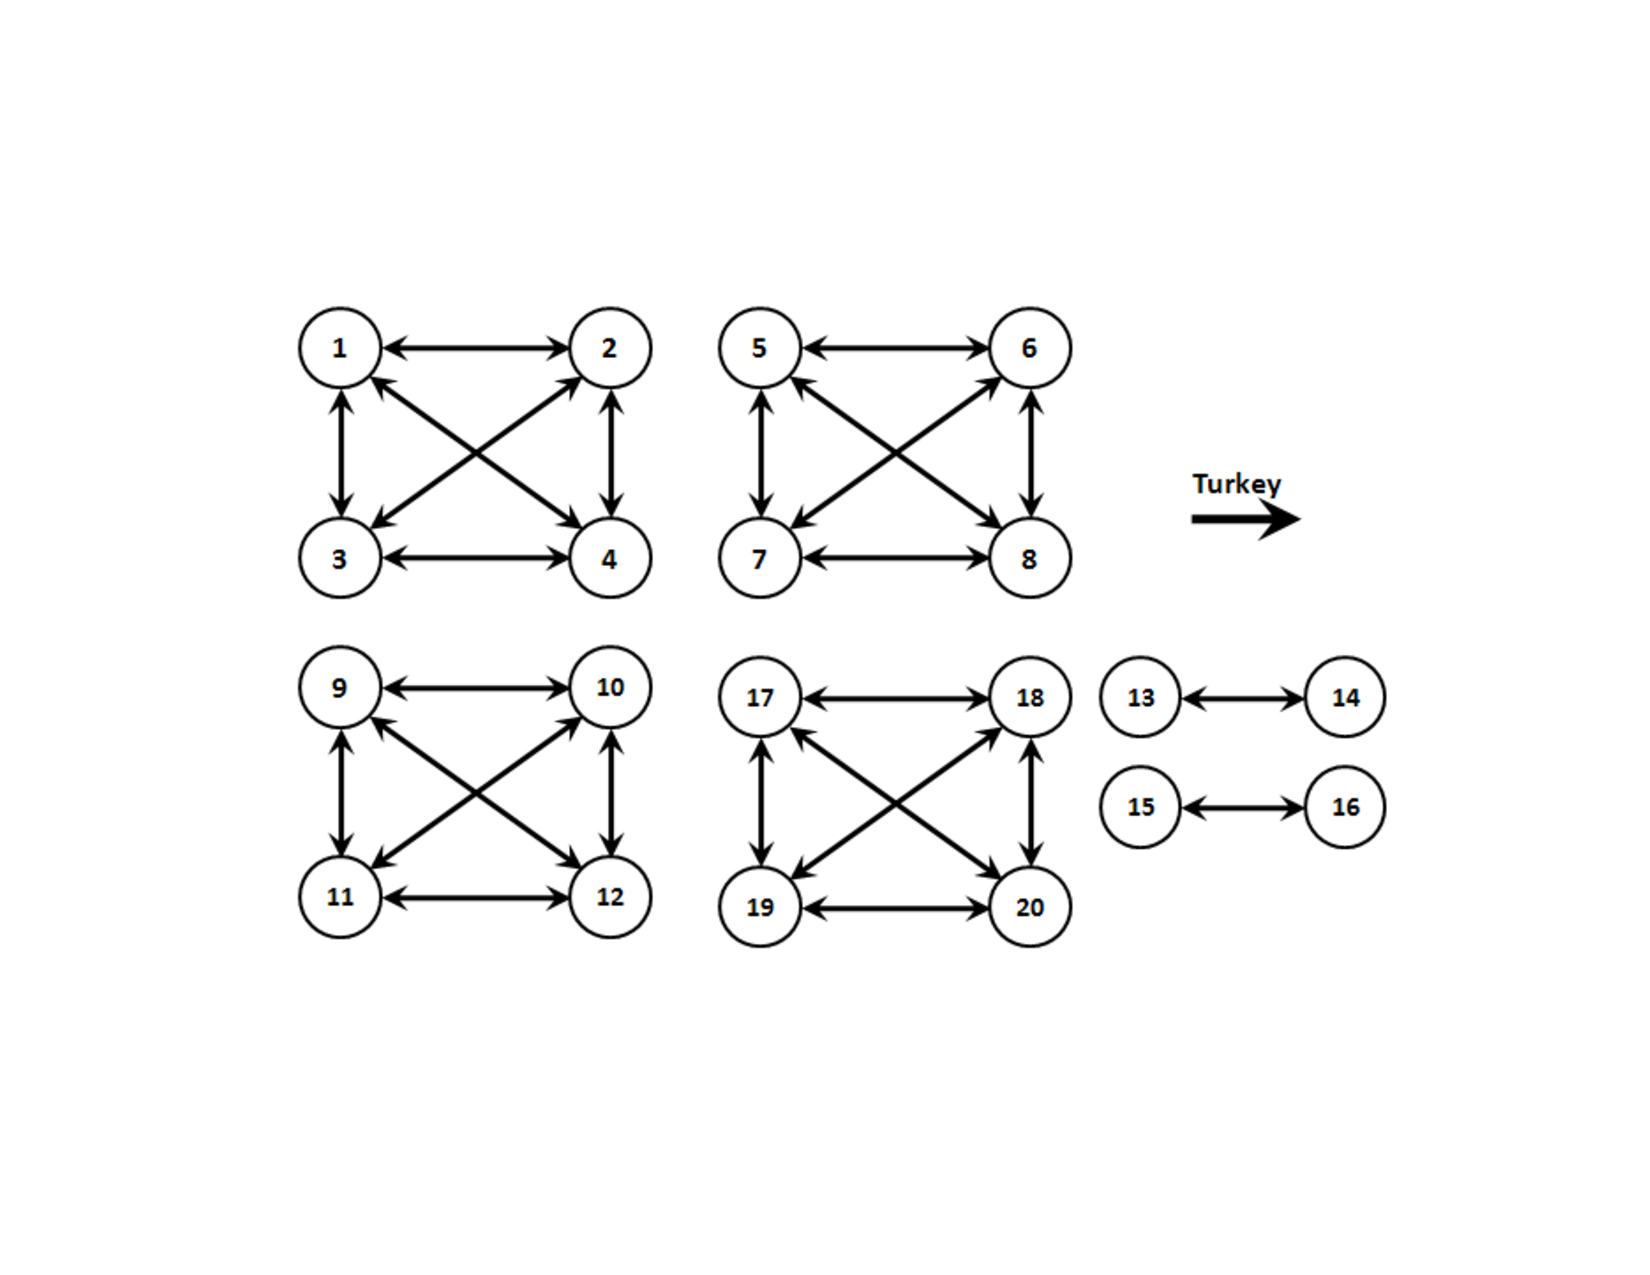
\includegraphics[scale=0.6]{PDF-IMG/tables/FIG4.pdf}

\caption{Graph Model of the 1990 conflict for movements by Turkey}

\label{fig:FIG4}
\end{figure}
\end{center}

\begin{center}
\begin{figure}[H]
\centering
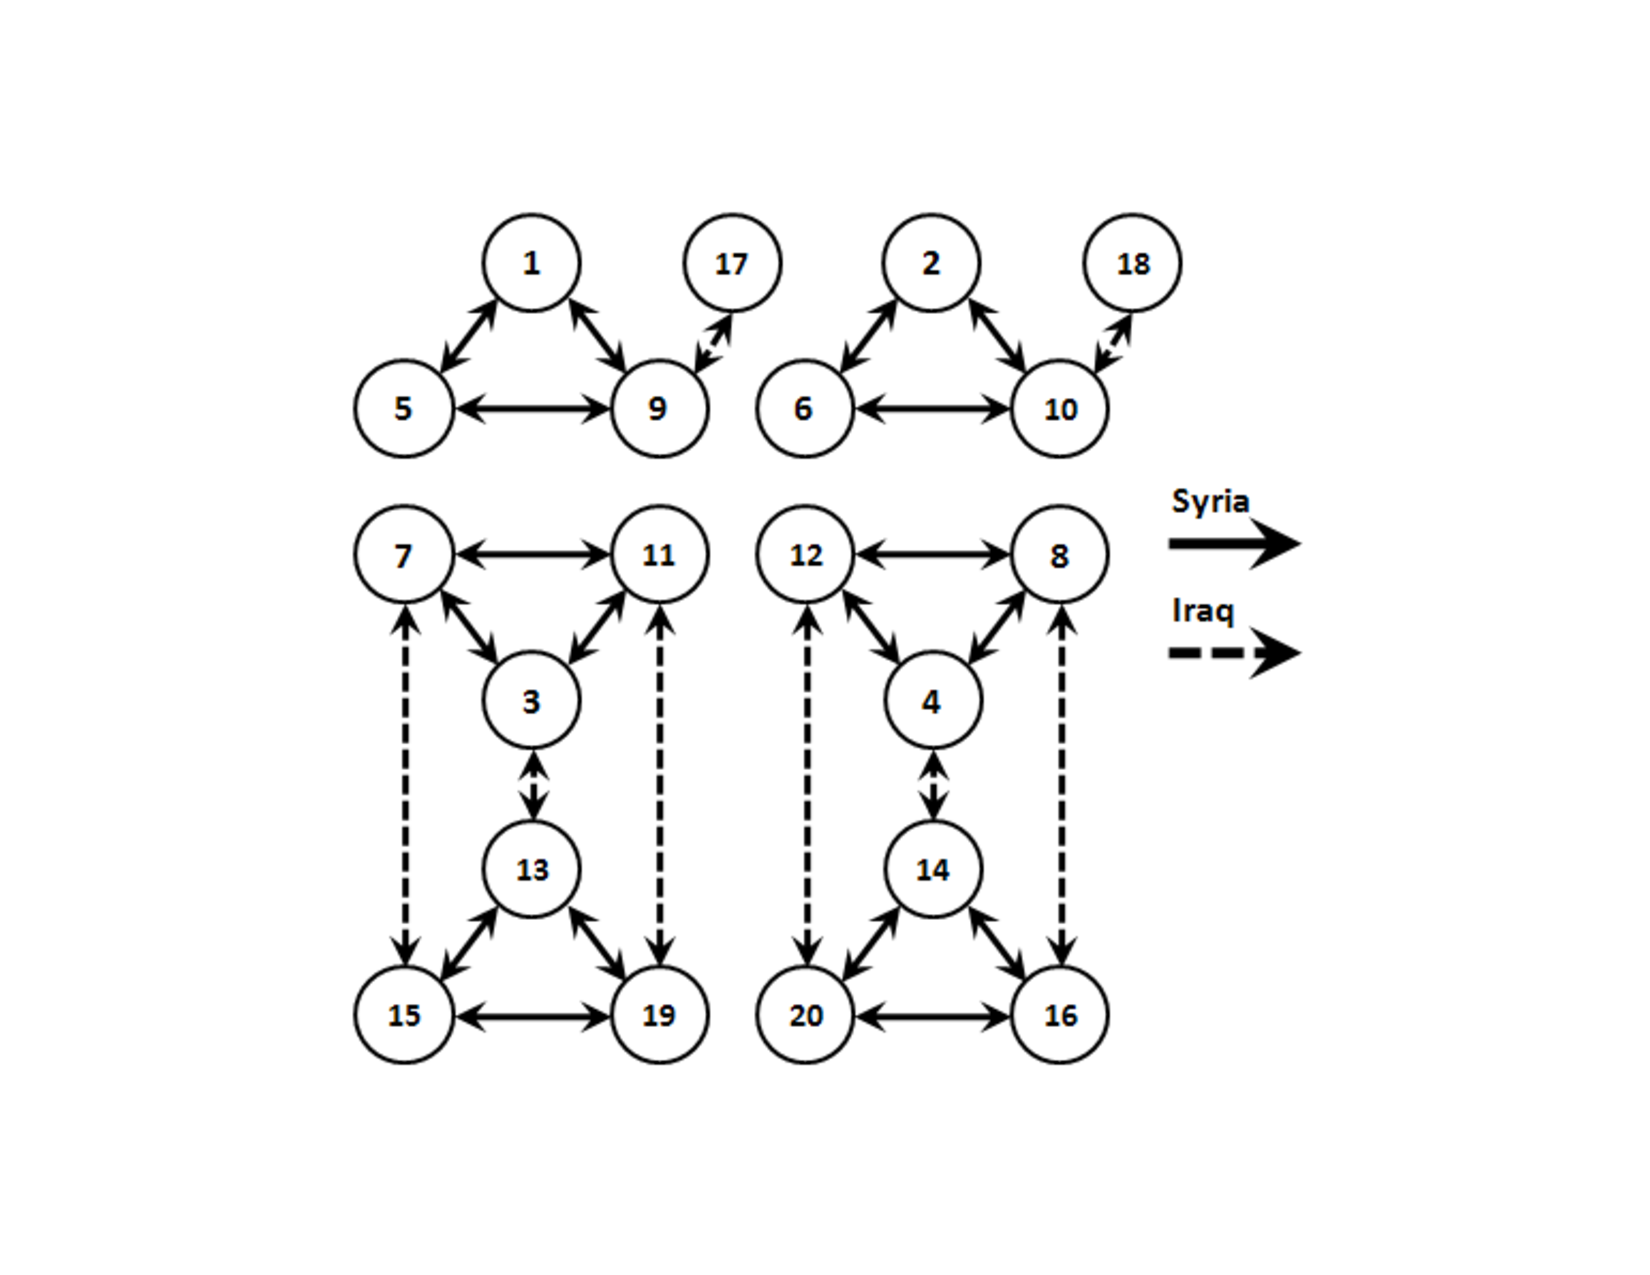
\includegraphics[scale=0.6]{PDF-IMG/tables/FIG5.pdf}

\caption{Integrated Graph Model of the 1990 conflict for both Syria and Iraq}

\label{fig:FIG5}
\end{figure}
\end{center}

\begin{center}
\begin{figure}[H]
\centering
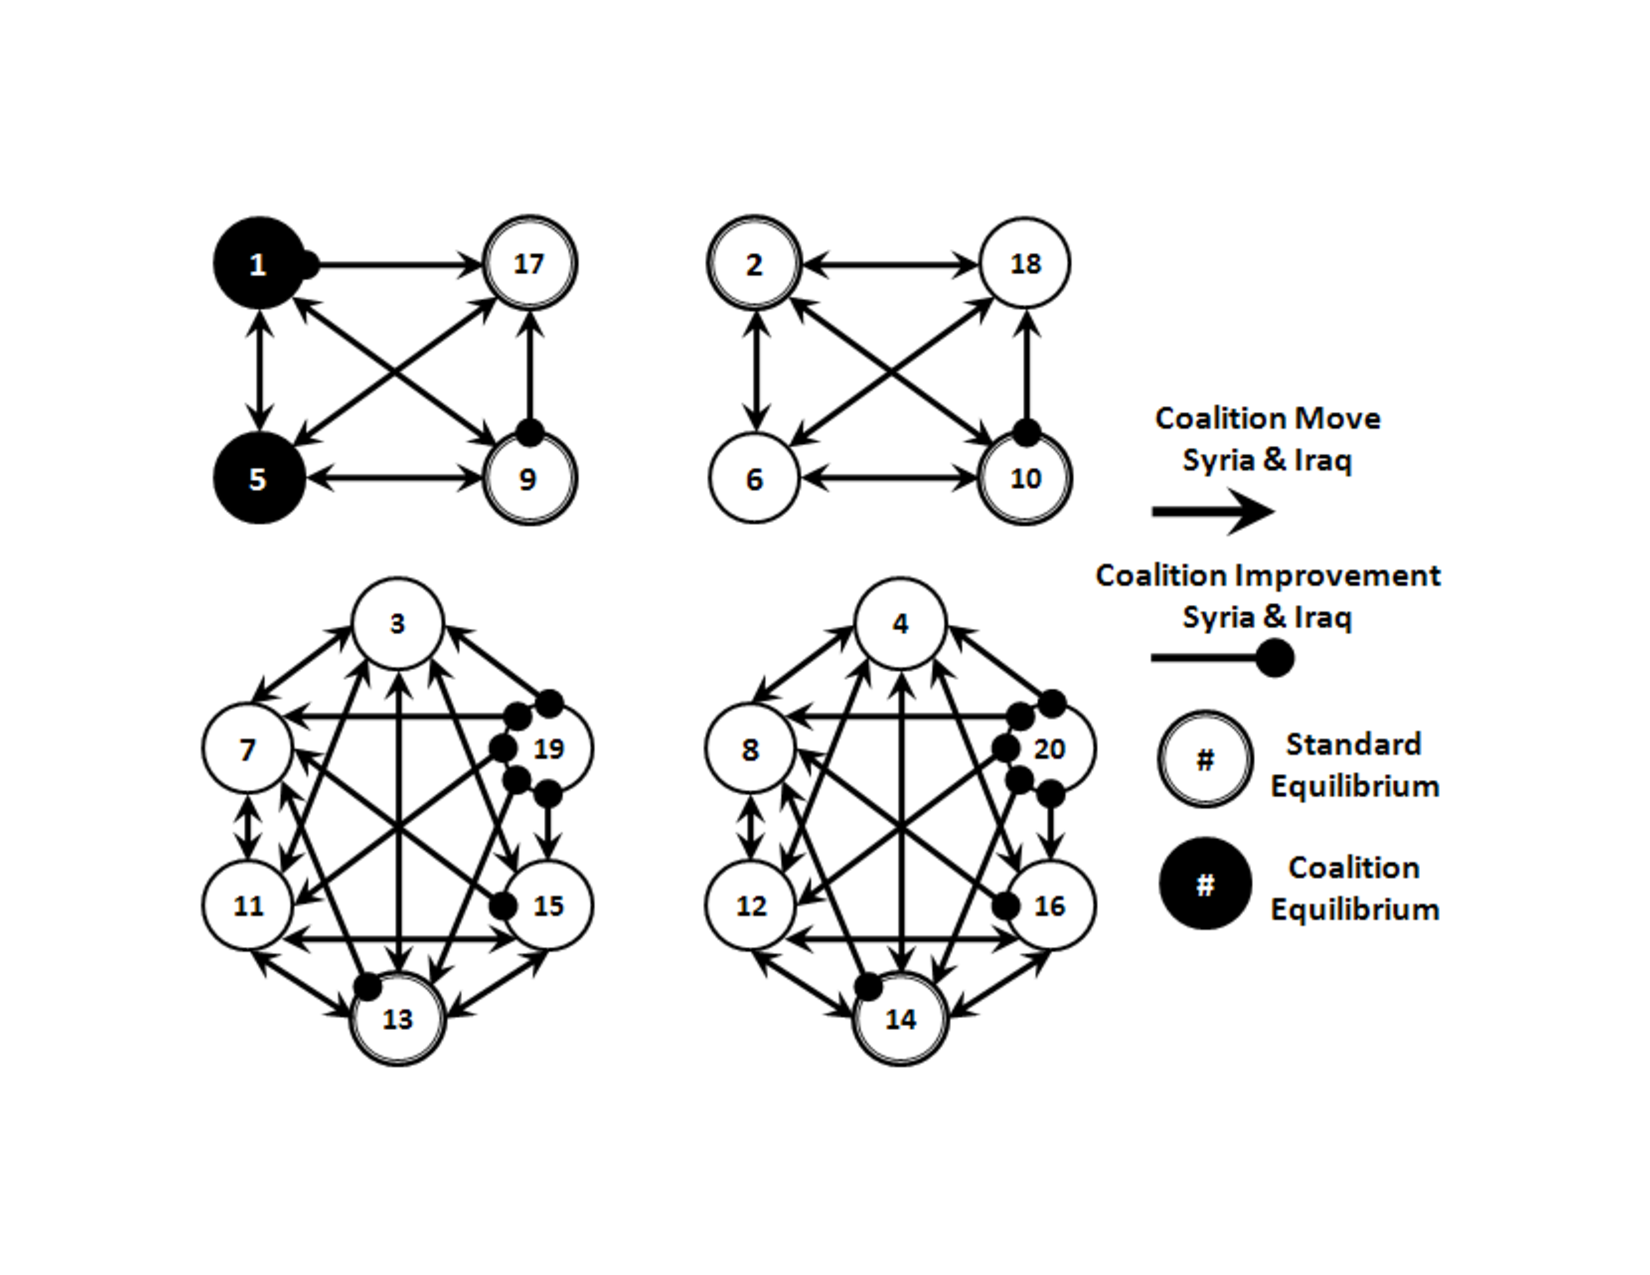
\includegraphics[scale=0.6]{PDF-IMG/tables/FIG6.pdf}

\caption{Coalition Graph Model of the 1990 conflict for a coalition of Syria and Iraq}

\label{fig:FIG6}
\end{figure}
\end{center}

Table \ref{tbl:Tables1990T14} presents the preference prioritization information for each DM of the 1990 conflict without the participation of the Third Party from most to least important. Table \ref{tbl:Tables1990T15} presents the ranking of states for all DMs in the conflict from most to least preferred. Equally preferred states are denoted by a bar above them. Table \ref{tbl:Tables1990T16} displays the equilibria results for each of the states after inputting the foregoing information into GMCR II. 

\begin{table}[H]
\centering
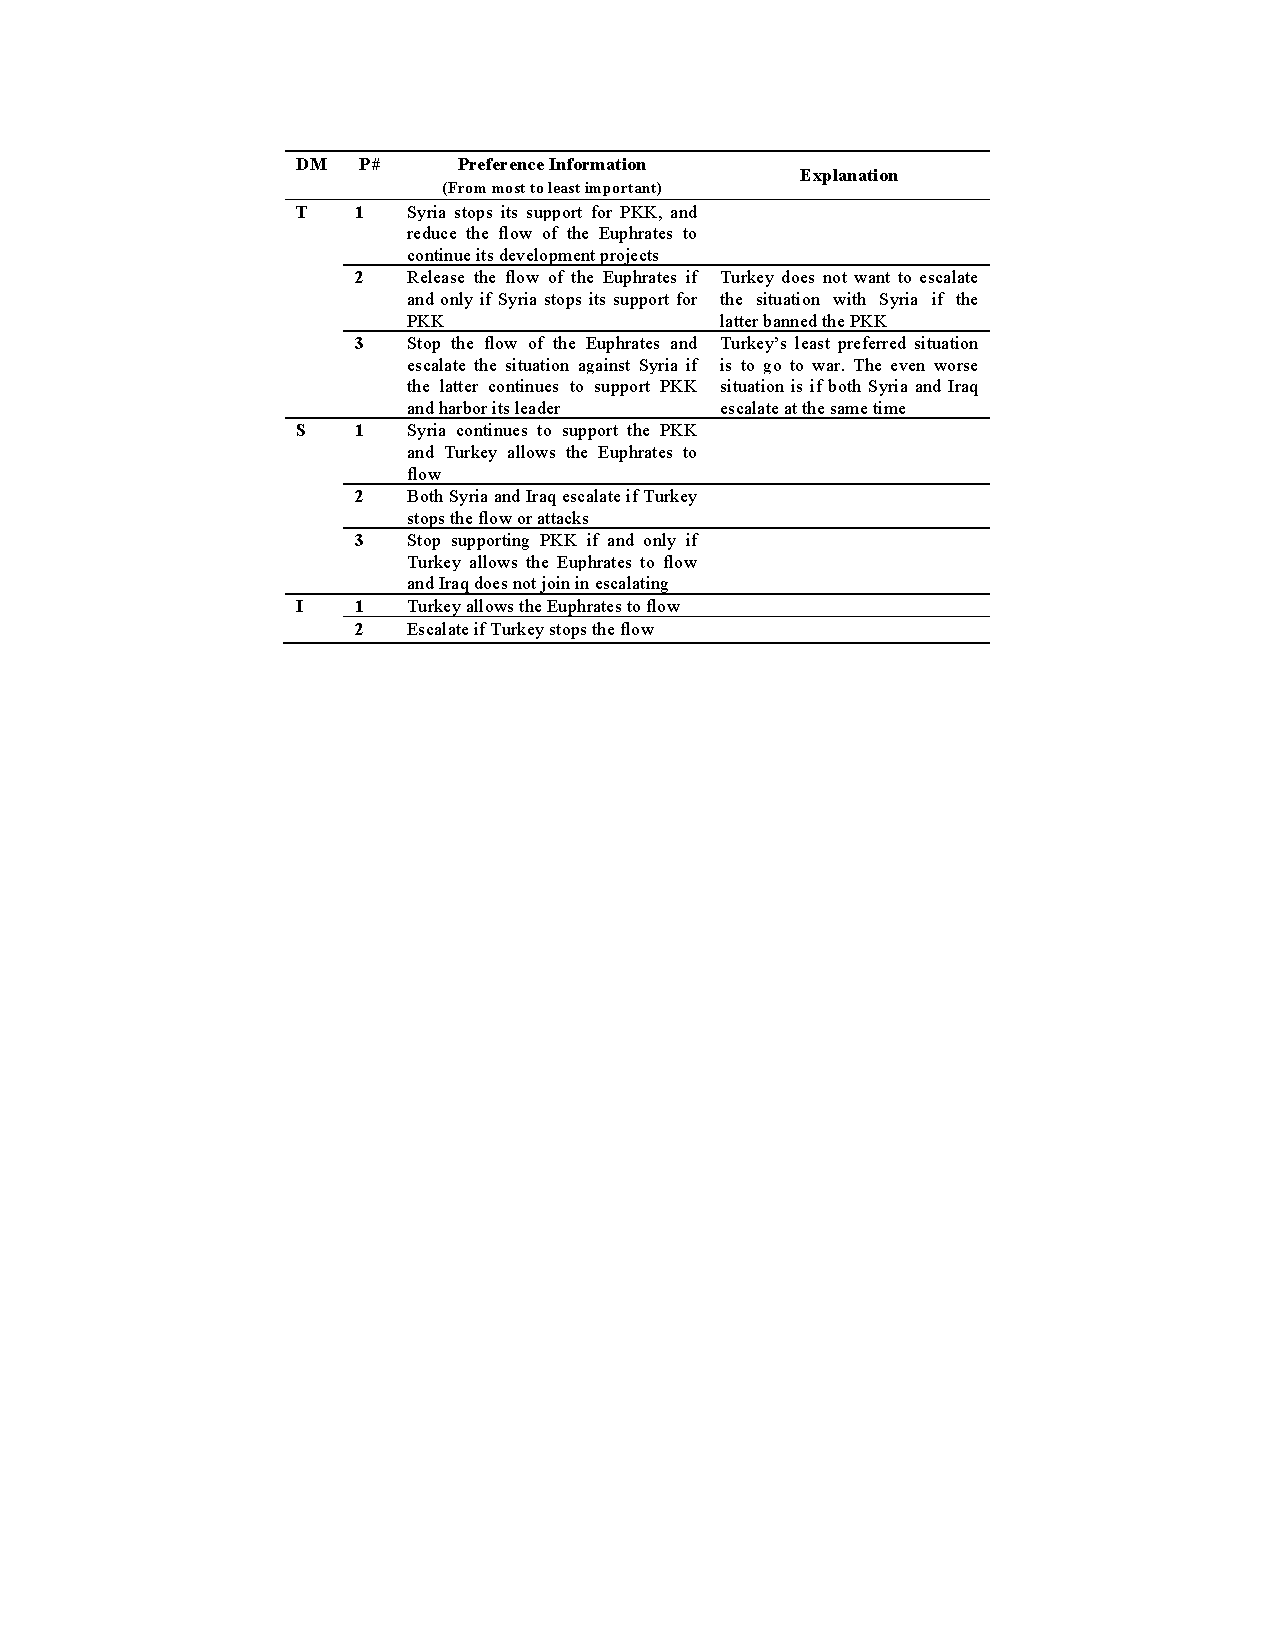
\includegraphics[scale=1]{PDF-IMG/tables/Tables1990T14.pdf}

\caption{Preference prioritization information for 1990 conflict}

\label{tbl:Tables1990T14}
\end{table}

\begin{table}[H]
\centering
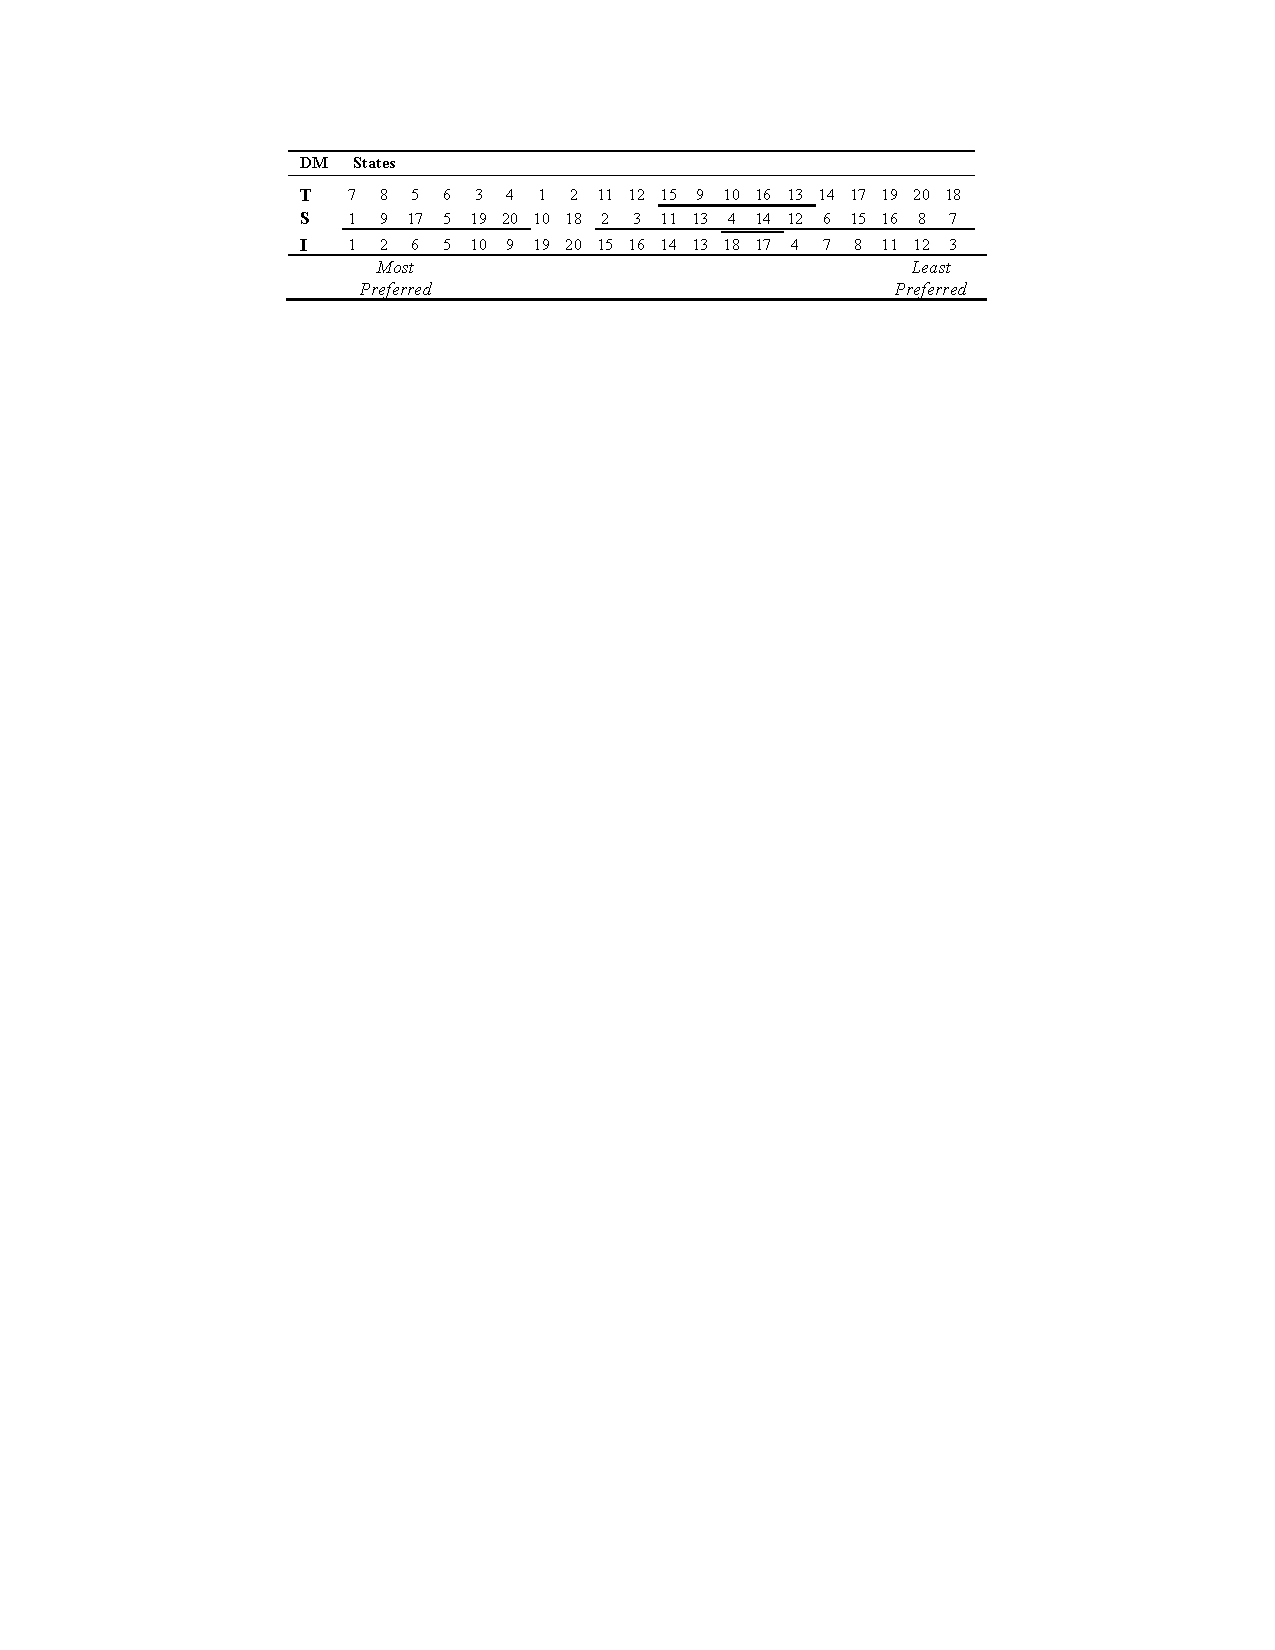
\includegraphics[scale=1]{PDF-IMG/tables/Tables1990T15.pdf}

\caption{Preference vector for DMs in the 1990 conflict}

\label{tbl:Tables1990T15}
\end{table}

\begin{table}[H]
\centering
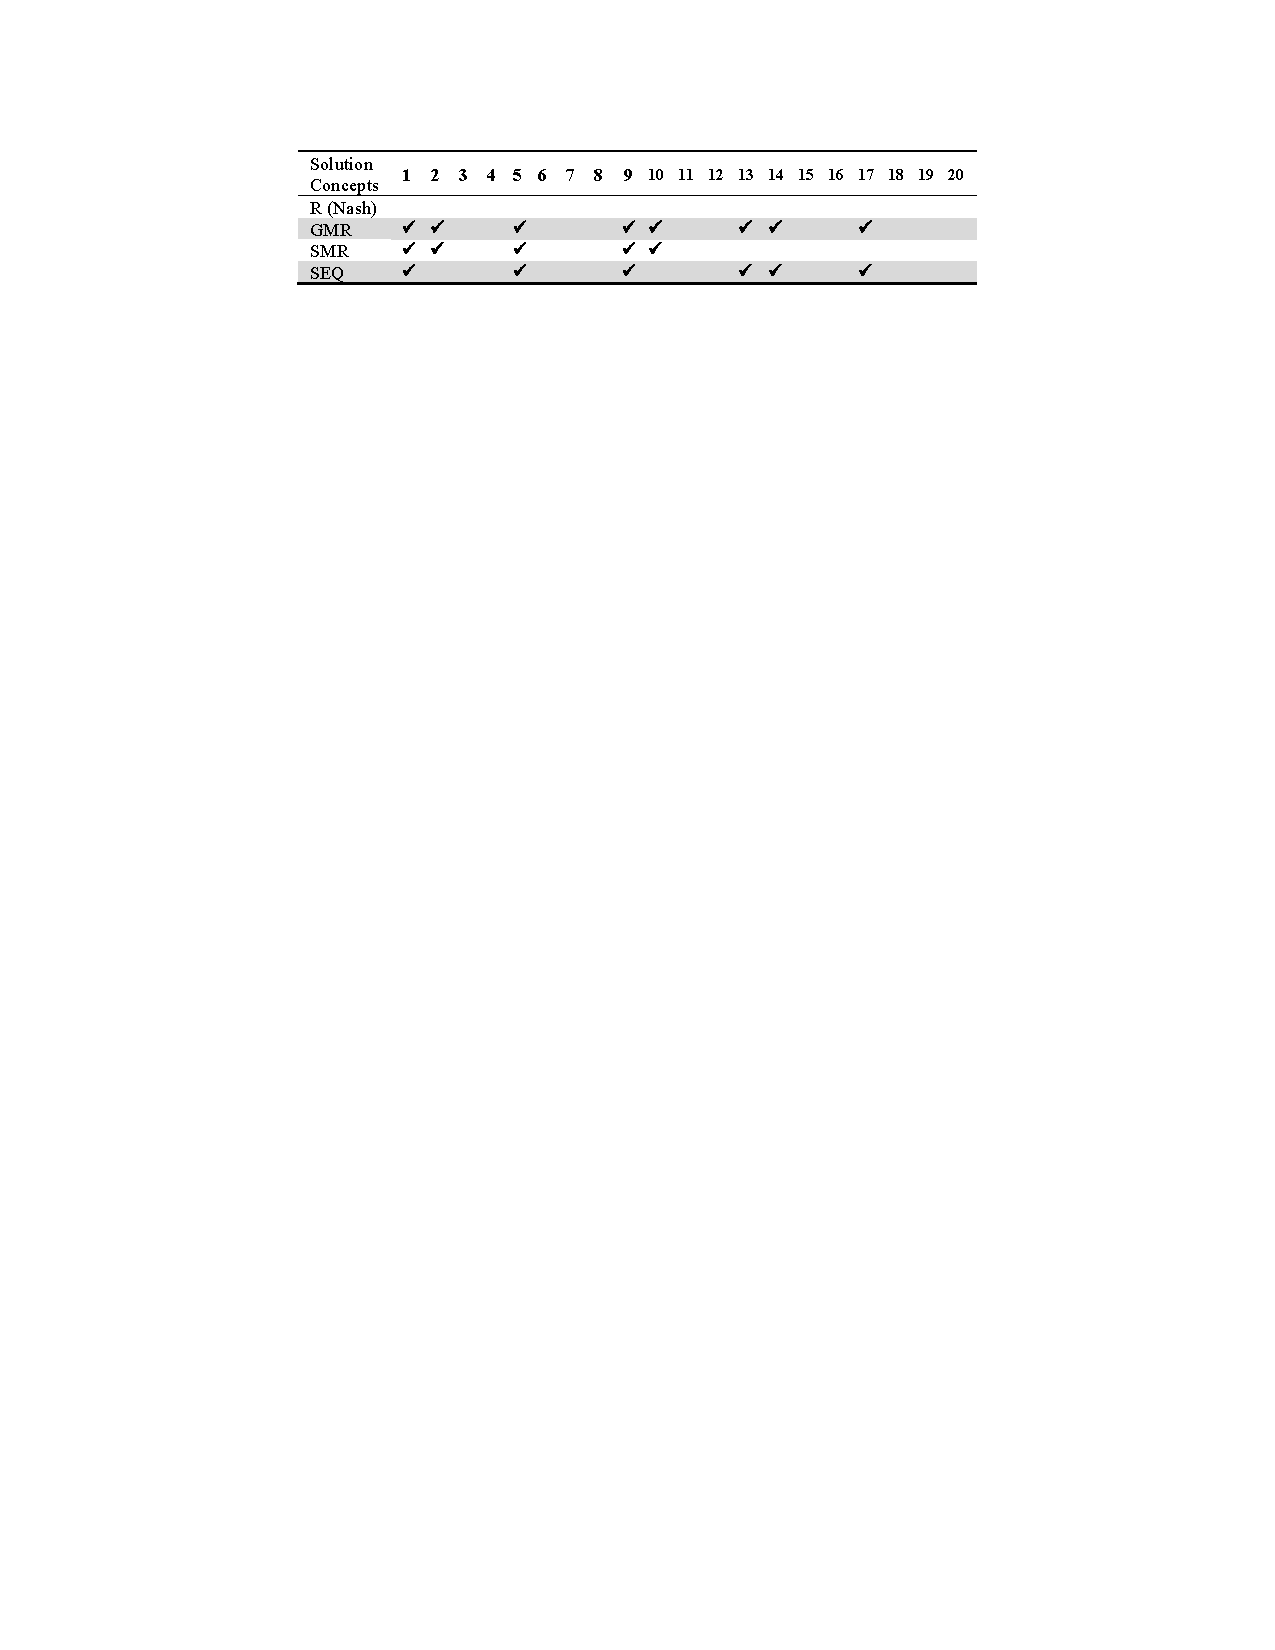
\includegraphics[scale=1]{PDF-IMG/tables/Tables1990T16.pdf}

\caption{Equilibria results for the 1990 conflict}

\label{tbl:Tables1990T16}
\end{table}

\subsection{In-depth coalition analysis}
In this subsection, a detailed coalition analysis is undertaken. The procedure for carrying out this analysis was adapted from \citet{kilgour2001coalition} and \citet{inohara2008a,inohara2008b}. The main steps of the procedure are now outlined briefly, while the detailed procedure can be found in the referenced articles. The first step is to construct the reachable lists $R_H(s)$ of all possible coalitions. This is illustrated in Table \ref{tbl:Tables1990T17}. For simplicity and to save space, Turkey, Syria and Iraq are abbreviated as T, S, and I, respectively. Similarly, the coalition between Turkey and Syria is abbreviated as TS, and so on. Next, one constructs the coalition improvement lists, denoted by $R_H^{(++)}(s)$, of possible coalitions. Table \ref{tbl:Tables1990T18} provides the results of this step.

\begin{sidewaystable}
\begin{table}[H]
\centering
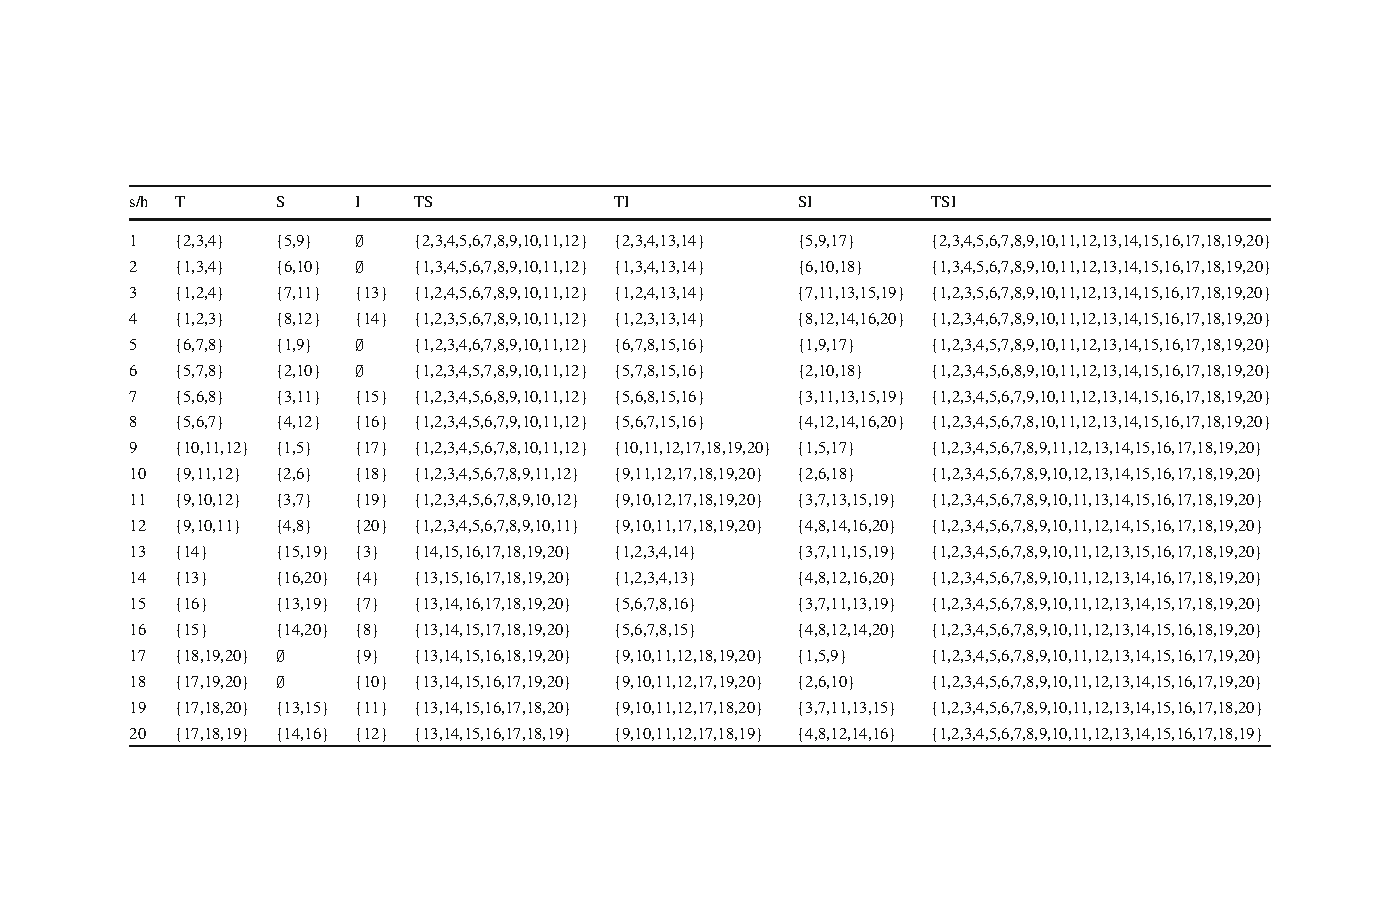
\includegraphics[scale=.97]{PDF-IMG/tables/Tables1990T17.pdf}

\caption{Reachable lists $R_H(s)$ for the 1990 conflict}

\label{tbl:Tables1990T17}
\end{table}
\end{sidewaystable}

\begin{table}[H]
\centering
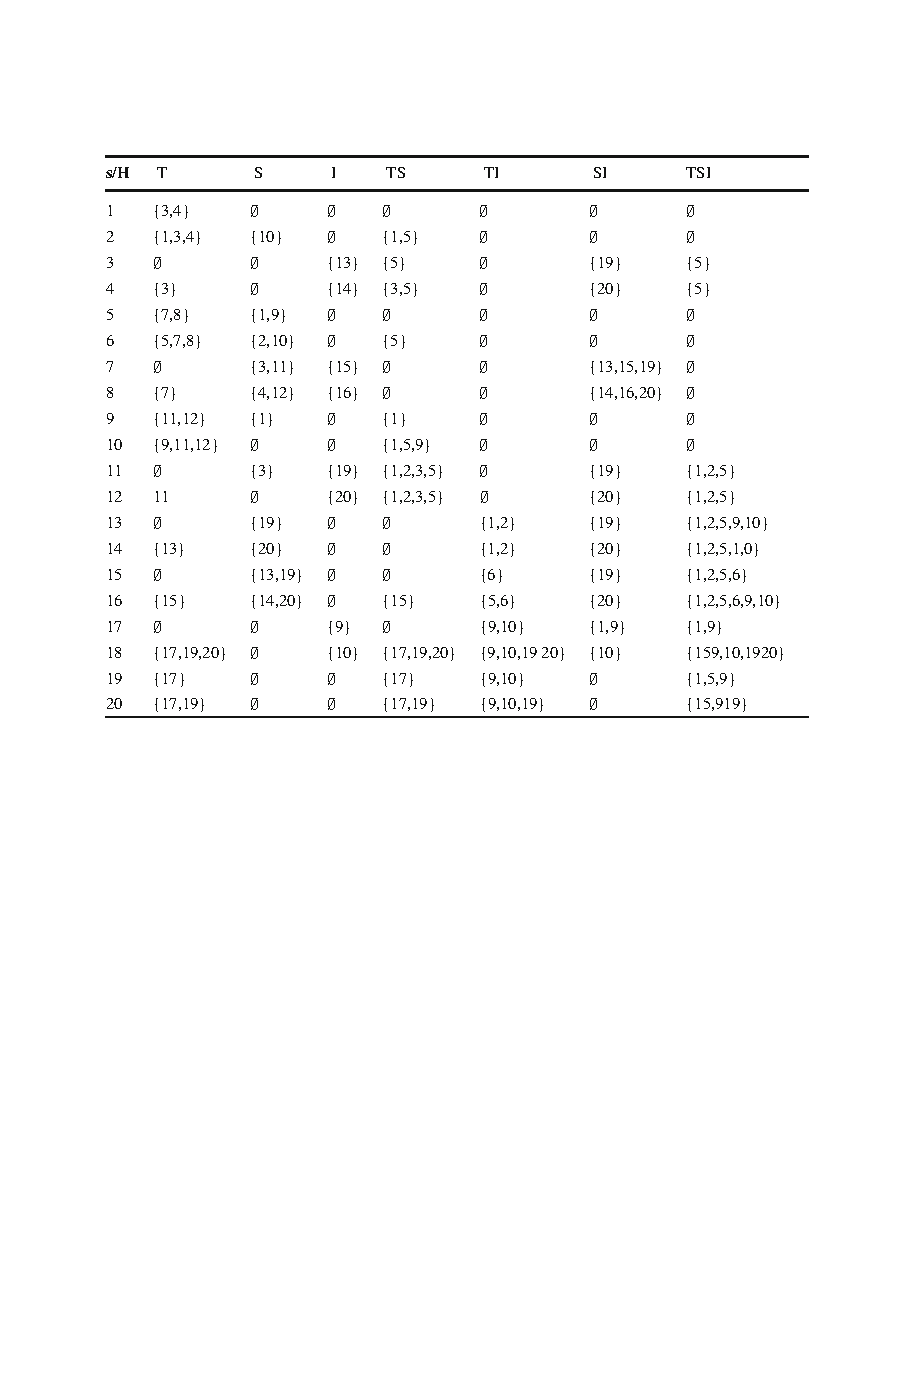
\includegraphics[scale=1]{PDF-IMG/tables/Tables1990T18.pdf}

\caption{Coalition improvement lists $R_H^{(++)}(s)$ for the 1990 conflict}

\label{tbl:Tables1990T18}
\end{table}

The third step is to construct the stability tableau. Table \ref{tbl:Tables1990T19} illustrates the construction of the table. The fourth step is to calculate the stability of each state for each DM according to the solution concepts with respect to the various coalitions. Notice that improvements written alone without squiggly parentheses (i.e.\{ \}) indicate unilateral improvements by that DM. Improvements written to the left of squiggly parentheses mean that these improvements are carried out with the coalition given within the squiggly parentheses. For example, from state 9, Turkey has a unilateral improvement to states 11 and 12. Turkey also has a coalition improvement from state 9 to 1 if it formed a coalition with Syria in this case and so on. 

Finally, to determine the coalition equilibrium according to a specific solution concept, the state under consideration should be stable for all of the DMs. In Table \ref{tbl:Tables1990T19} the conflict is examined according to both CNash (i.e. Coalition Nash Stability) and CSEQ (i.e. Coalition Sequential Stability). The coalition stability is a generalization of the individual stability. Other solution concepts can be assessed as well. However, as this conflict is fairly large and contains 20 states, the analysis is limited to these two solution concepts. 


\begin{table}[H]
\centering
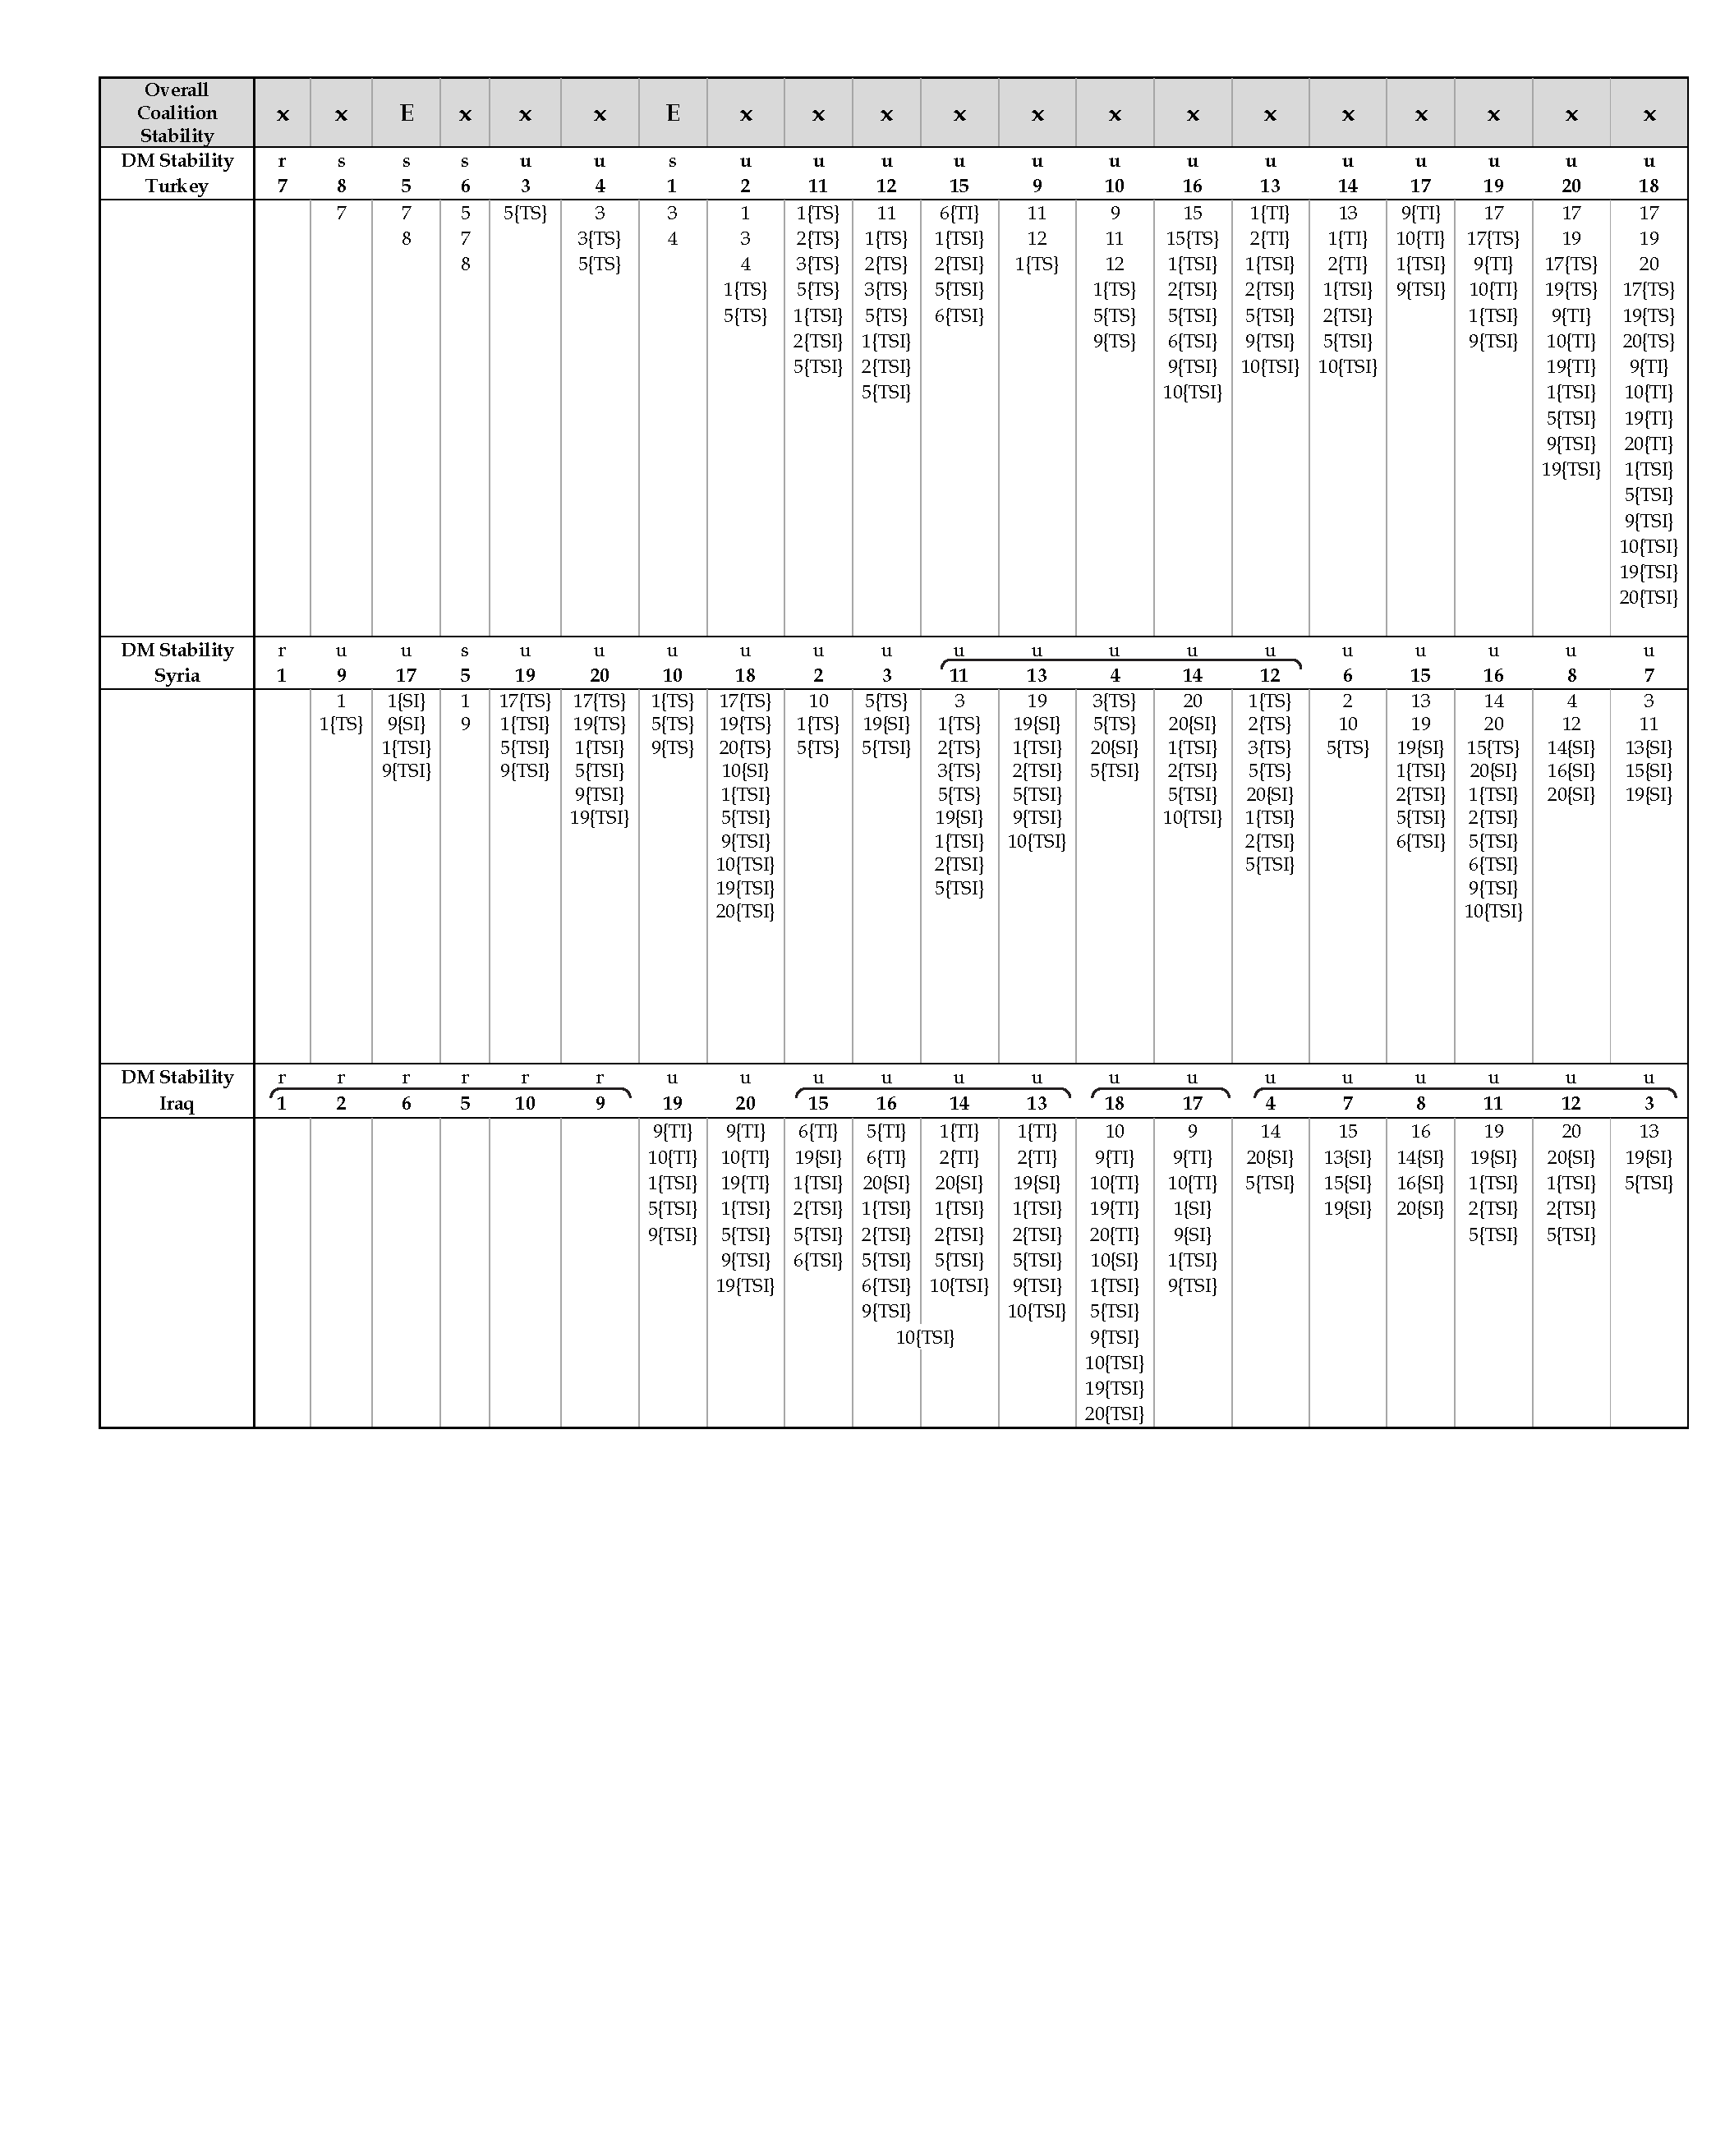
\includegraphics[scale=.5]{PDF-IMG/tables/Tables1990T19.pdf}

\caption{Stability analysis tableau for coalition sequential stability for the 1990 conflict}

\label{tbl:Tables1990T19}
\end{table}

\subsection{Insights on the 1990 conflict}
Although no rational (Nash) coalition stability is present in this conflict, states 1 and 5 are sequentially stable by coalition sanctioning and, therefore, one can confidently state that the conflict will end up at one of these two states. Historically, the conflict concluded at state 1, as will be described in the evolution of the conflict.

The construction of the different types of Graph Models in Figures 4, 5, and 6 give a very clear understanding of the conflict and how it can evolve by unilateral moves by each DM as well as by a coalition. This forms a framework to communicate the conflict to stakeholders. Moreover, different moves and counter-moves can be easily assessed and compared especially in a complicated conflict like this one.
From the analysis given in Table \ref{tbl:Tables1990T16}, one can see that there is no rational Nash stable state. However, three states have fairly strong equilibria by sequential sanctioning and symmetric metarationality: states 1, 5, and 9. These states represent the status quo, banning PKK, and escalating the situation unilaterally by Syria. An examination of these results eliminates the possibility of forming a coalition, which happened historically, and none of these equilibria includes escalation by Iraq.

After performing the in-depth coalition analysis, no new equilibrium jump is introduced but coalition moves can be spotted and taken into account. The lesson learned from this conflict is that one should account for coalition moves and improvements. The historical evolution of the conflict (\ref{tbl:Tables1990T20}) shows how Turkey?s action formed a coalition between the bitter enemies, Syria and Iraq, forcing Turkey to revert to the status quo equilibrium. Furthermore, in complicated conflicts like this one, one must be very careful to choose the right preference information as the conflict resolutions can be highly sensitive to preferences. This is especially true when many political factors are considered.

\begin{table}[H]
\centering
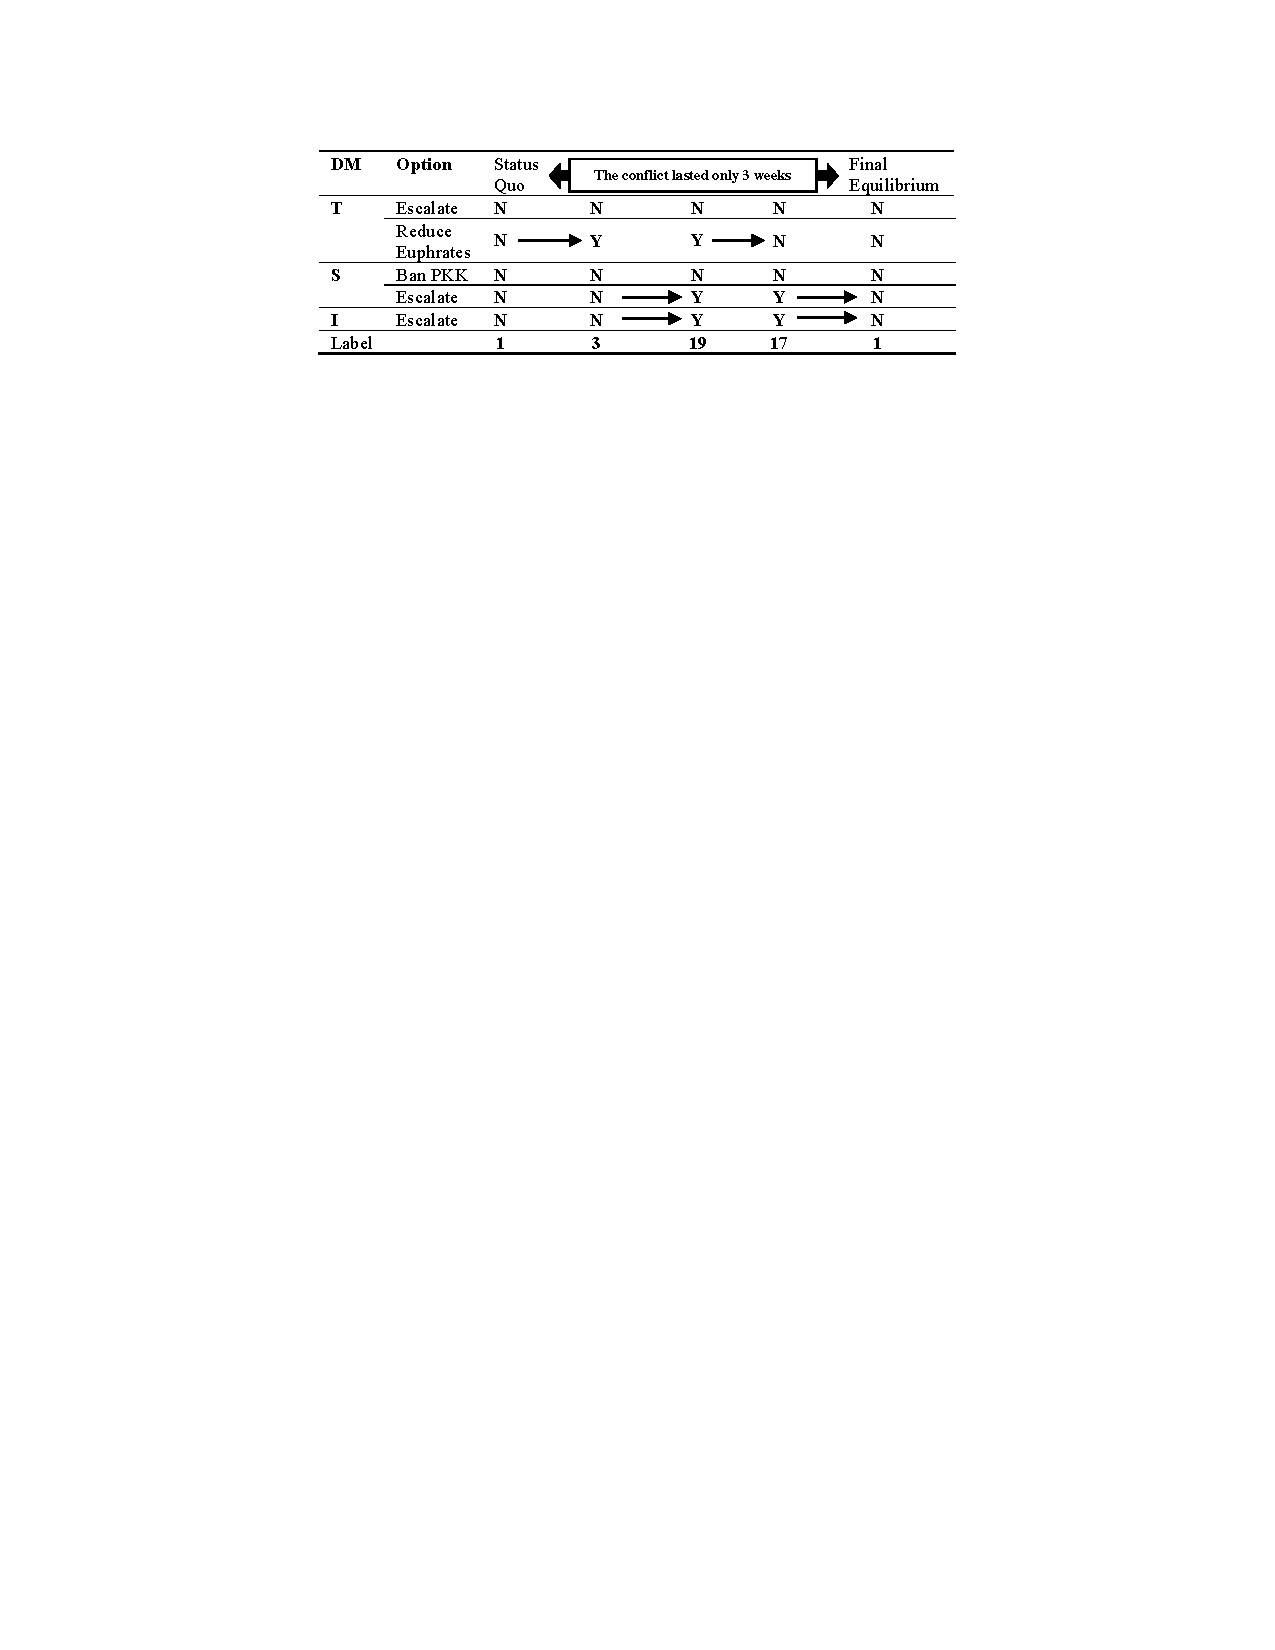
\includegraphics[scale=1]{PDF-IMG/tables/Tables1990T20.pdf}

\caption{Historical evolution of the 1990 conflict}

\label{tbl:Tables1990T20}
\end{table}

\section{Strategic Investigation of the 1998 Controversy}
The DMs and options for the 1998 conflict are given in Table \ref{tbl:t11}. Turkey has two options: escalate the situation against Syria or carry out a full invasion. Syria has two options of stopping its support for the PKK or escalating the situation. The third party, Egypt, has a single option of acting or not.

\begin{table}[H]
\centering
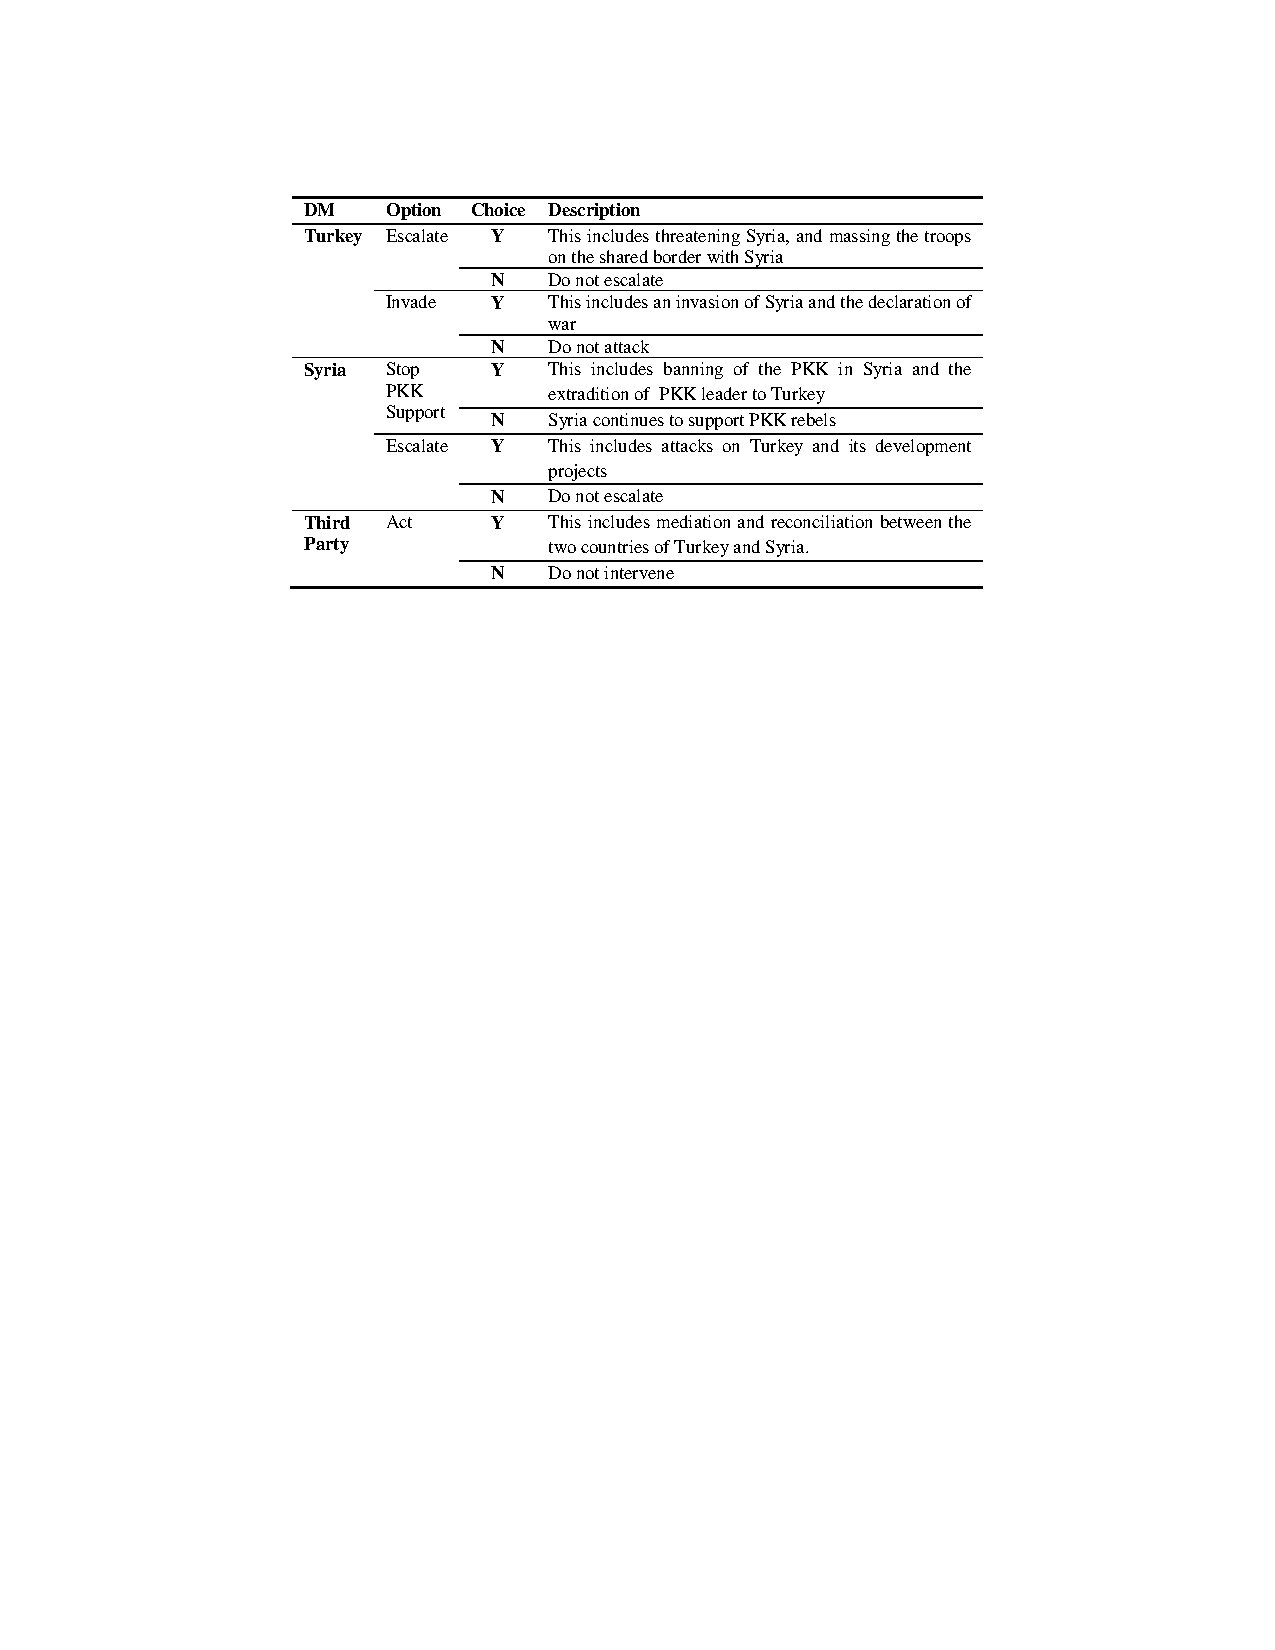
\includegraphics[scale=1]{PDF-IMG/tables/11.pdf}

\caption{DMs, options and descriptions for the 1998 conflict}

\label{tbl:t11}
\end{table}

The set of feasible states is provided in Table \ref{tbl:t12}. Note that there is one infeasible situation in which Syria can both ban PKK and escalate at the same time (mutually exclusive options). Also notice that state 9 is an indistinguishable state if Turkey decides to invade Syria, since a full scale war will occur and the game will end.  Because the third party played an Arbitrator role in this conflict, the situation in which it acts and Syria does not ban the PKK, is removed. The remaining possible states or scenarios are provided in Table \ref{tbl:t12}. Figure \ref{fig:SyTrGM} shows the Integrated Graph Model of the conflict.

\begin{table}[H]
\centering
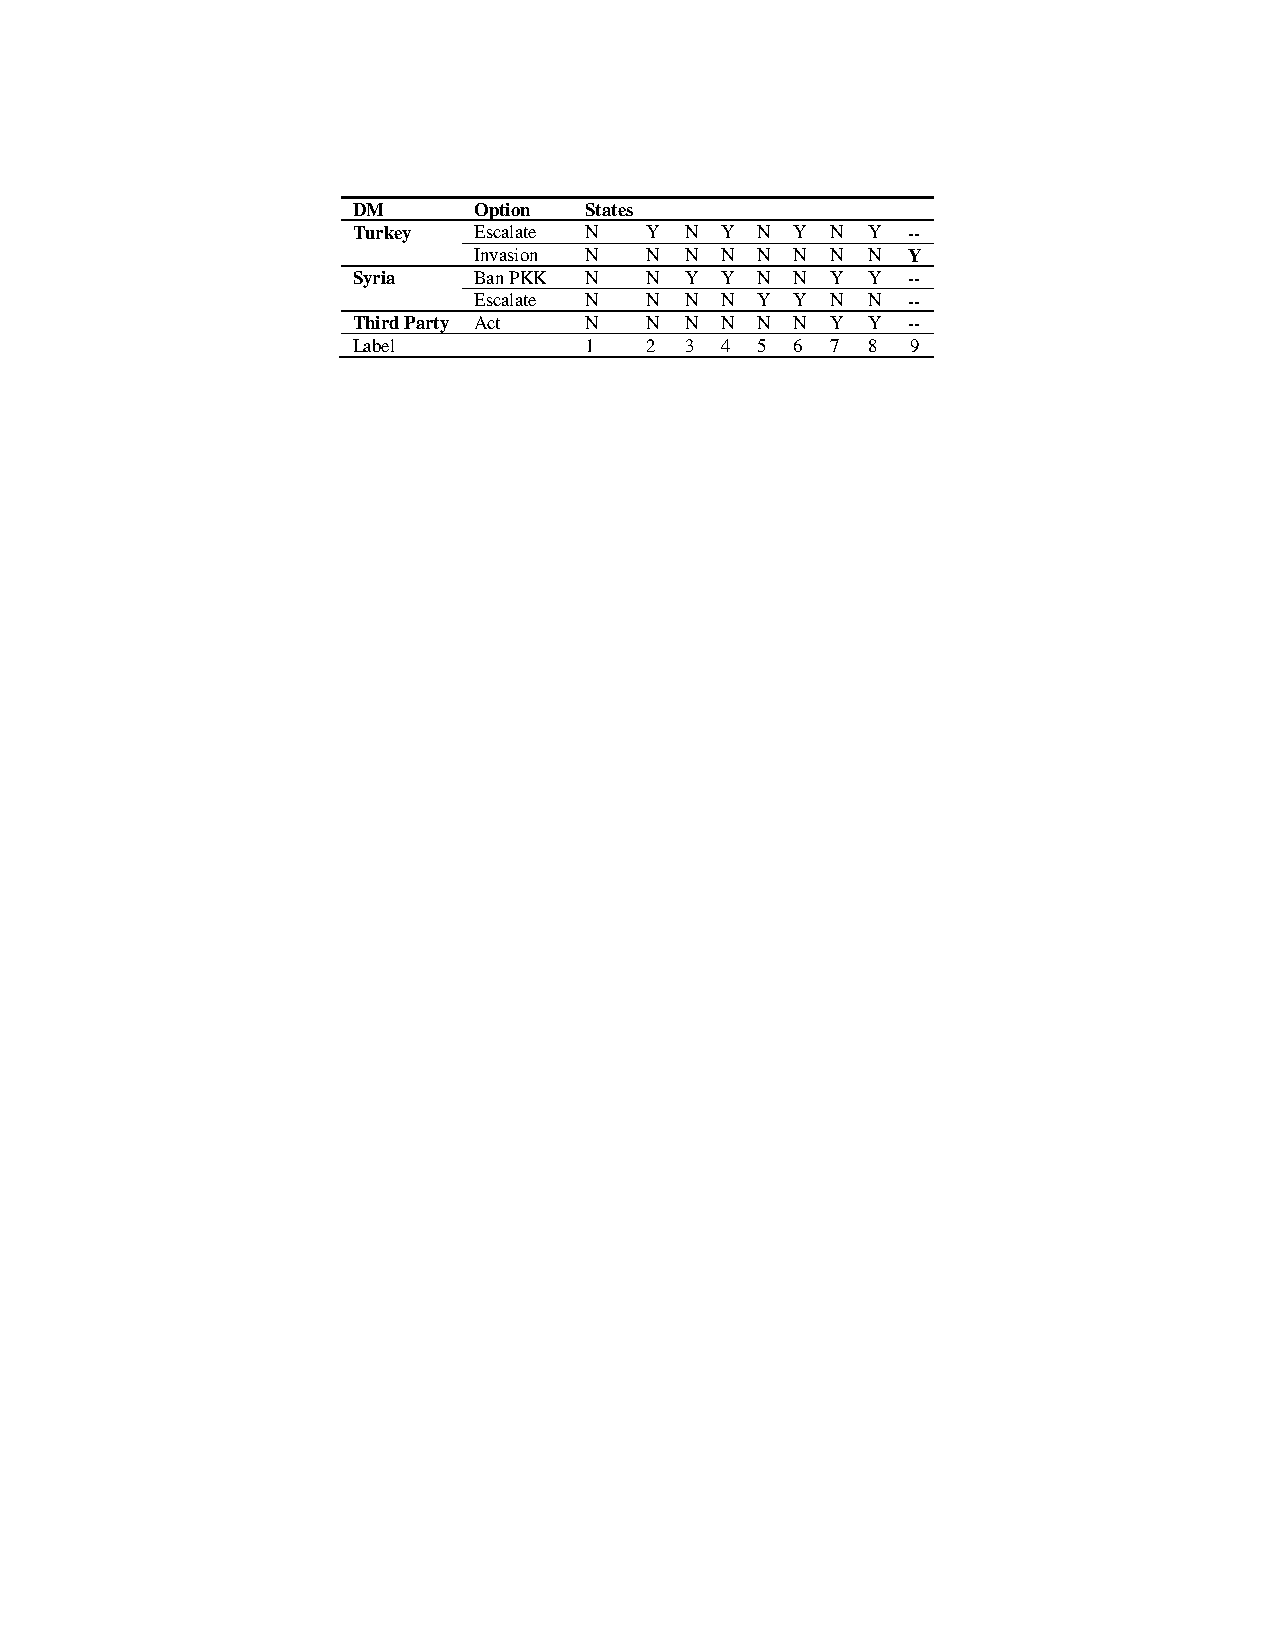
\includegraphics[scale=1]{PDF-IMG/tables/12.pdf}

\caption{DMs, options and states for the 1998 conflict with the third party}

\label{tbl:t12}
\end{table}

\begin{center}
\begin{figure}[H]
\centering
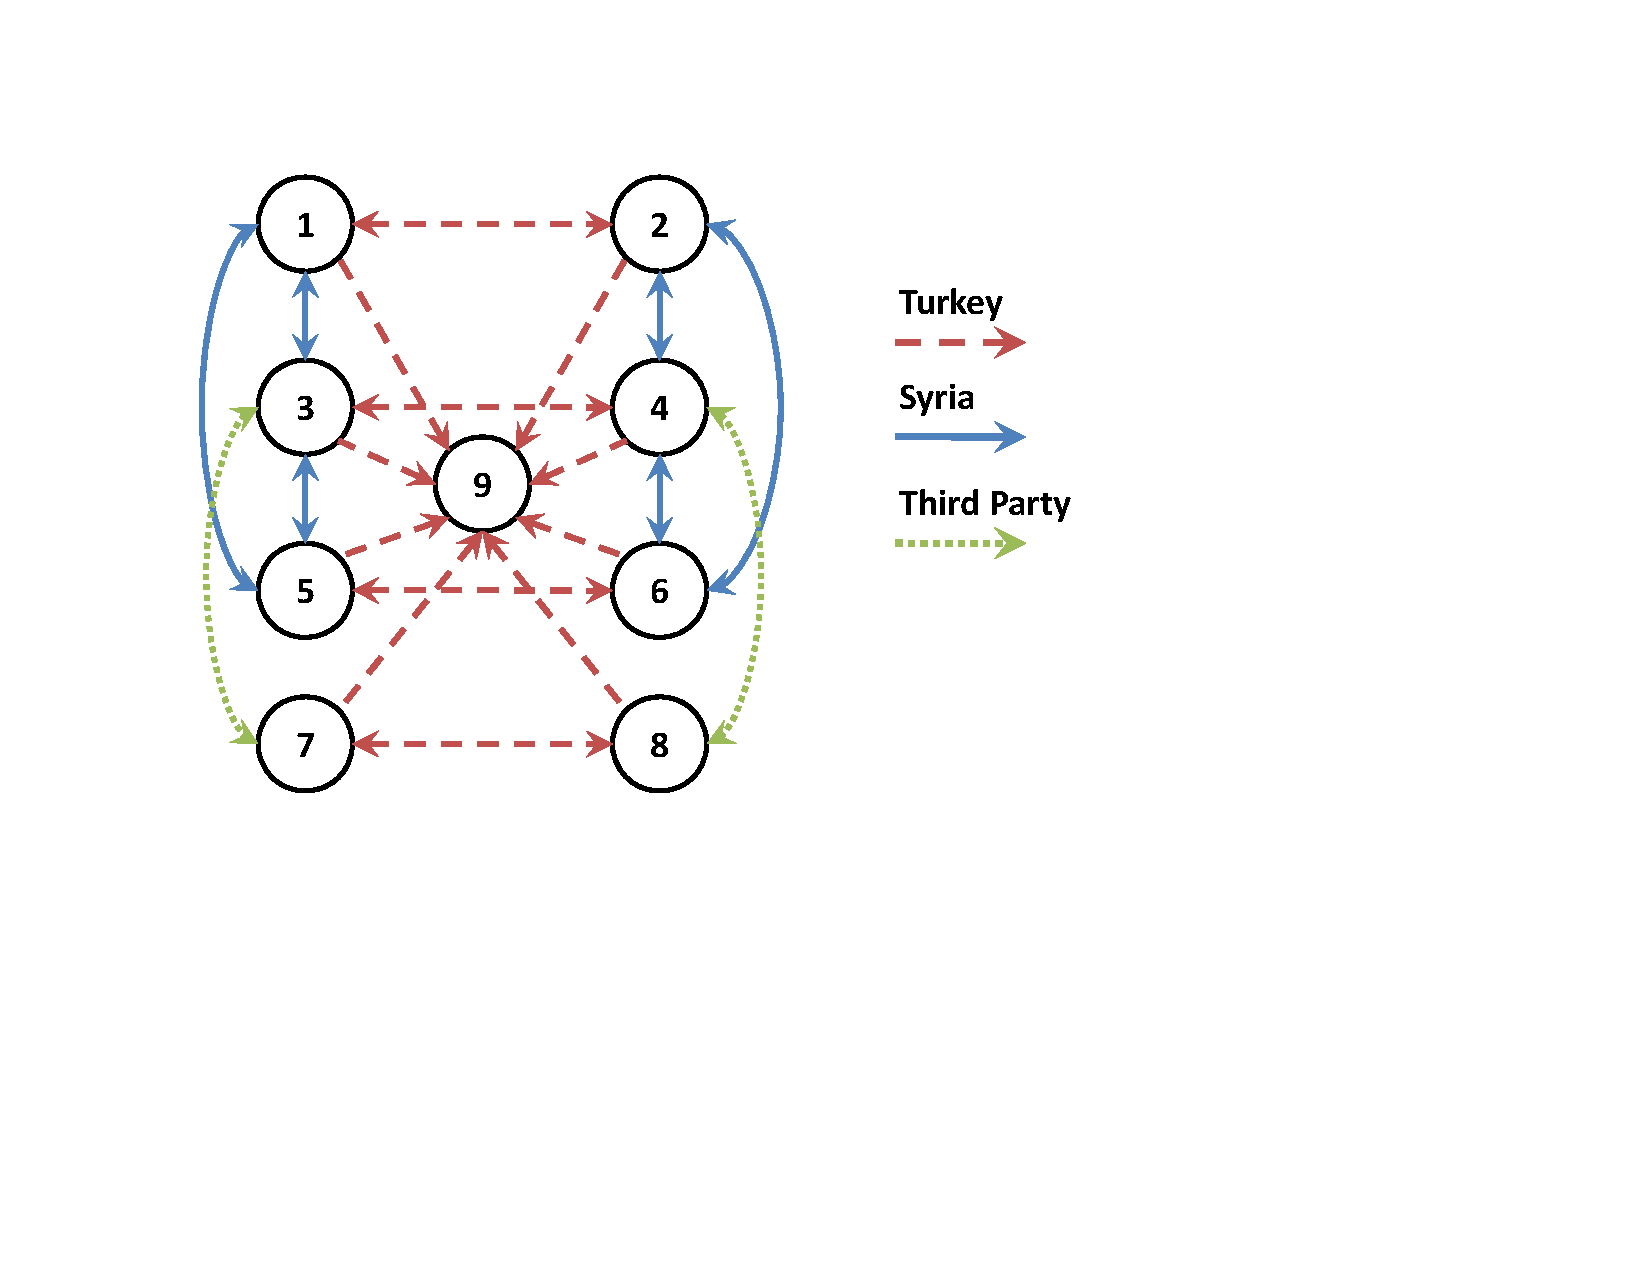
\includegraphics[scale=0.6]{PDF-IMG/SyTrEg.pdf}

\caption{Integrated Graph Model of the 1998 conflict with the third party}

\label{fig:SyTrGM}
\end{figure}
\end{center}

In this situation, the third party acts as an Arbitrator, since the party has the power to exclude some states \citep{sakamoto2005}. In this conflict, the third party, Egypt, restricted Syria's move of not banning the PKK if it intervened. Egypt brings to the table legitimacy and extensive experience gained through experience with the conflicts along the Nile basin \citep{akanda2007tigris}. Syria was united with Egypt under the United Arab Republic (UAR) before Syria declared independence from the UAR in the 1970s. UAR was mostly led by the Egyptian President, Gamal Abdel Nasser. These factors combined to give Egypt a say in Syria's politics. Table \ref{tbl:t13} presents the preference prioritization information for each DM in the 1998 conflict from most to least preferred. Table \ref{tbl:t14} presents the hierarchical preference statements for Turkey, Syria, and the third party from most to least important. Table \ref{tbl:t15} outlines the analysis results after inputting the foregoing information into GMCR II. 

\begin{table}[H]
\centering
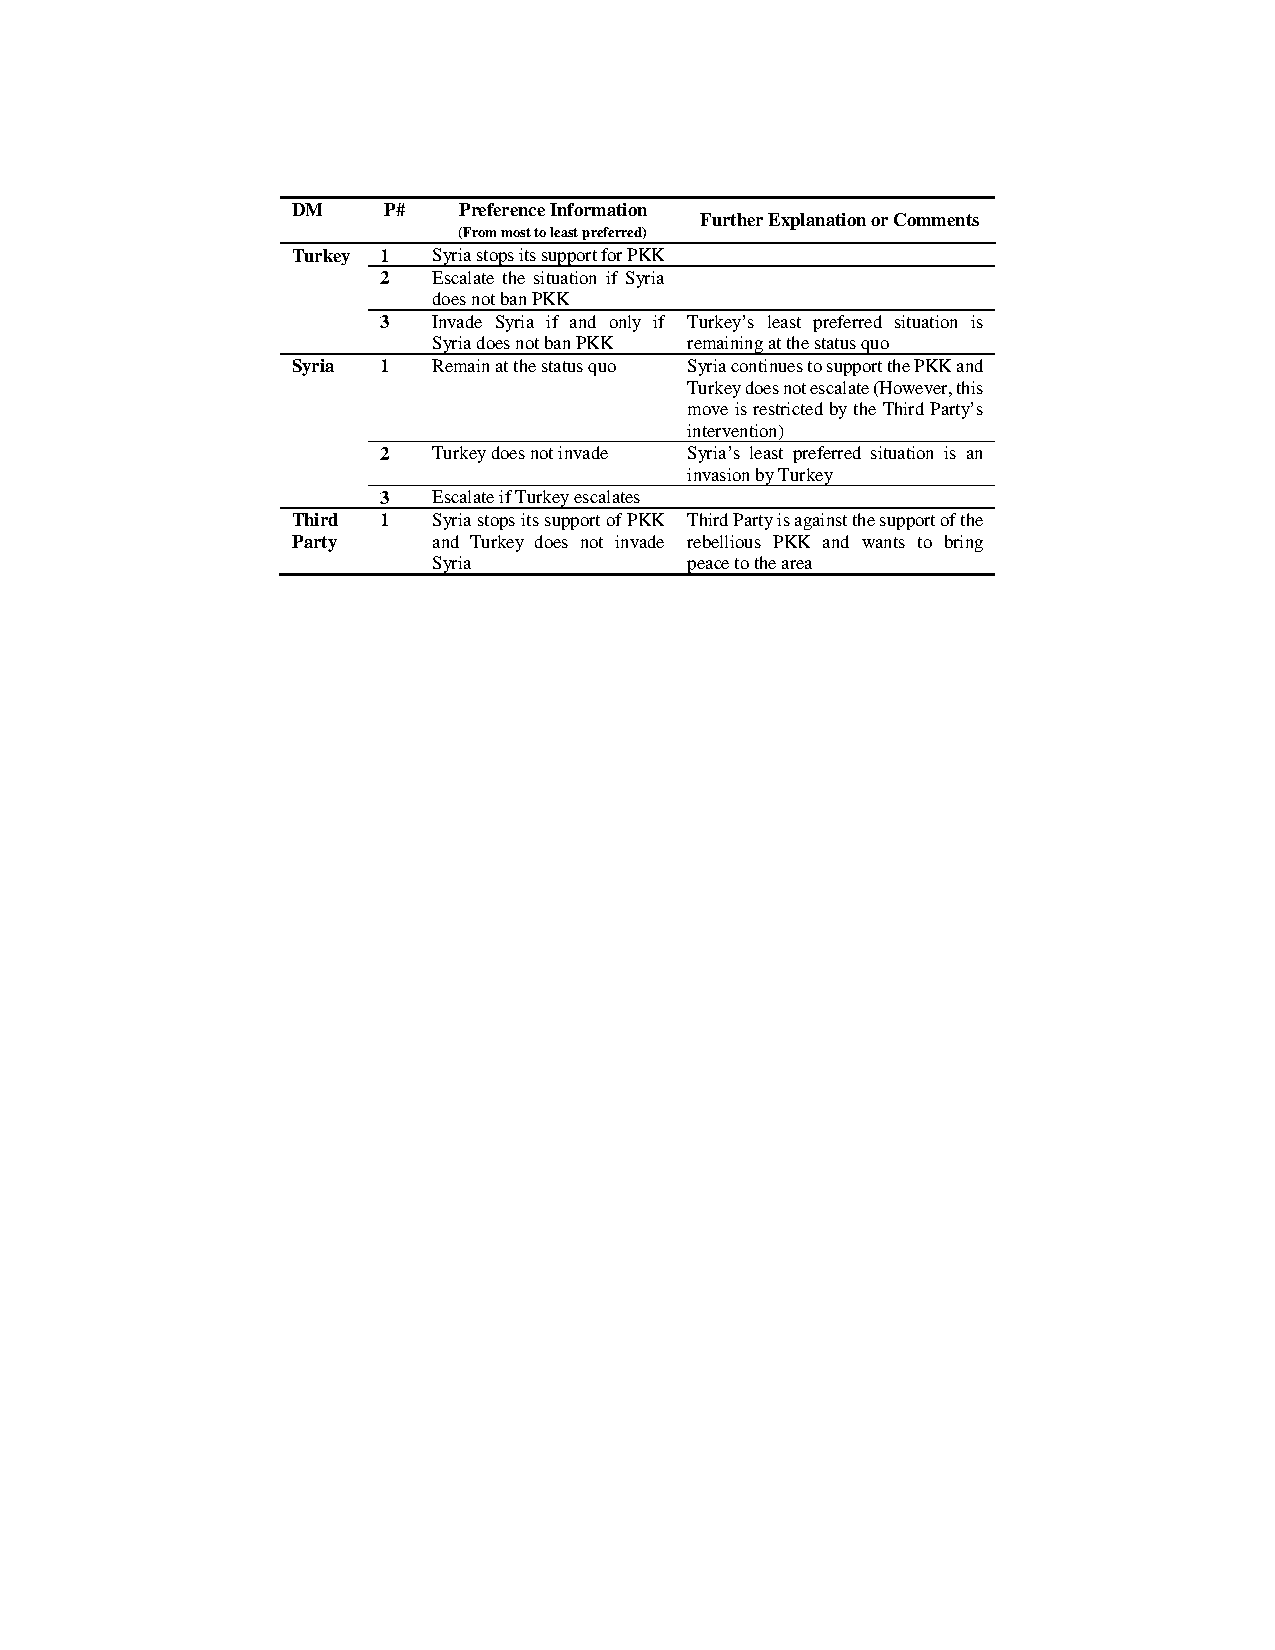
\includegraphics[scale=1]{PDF-IMG/tables/13.pdf}

\caption{Preference prioritization information for the 1998 conflict with the third party}

\label{tbl:t13}
\end{table}

\begin{table}[H]
\centering
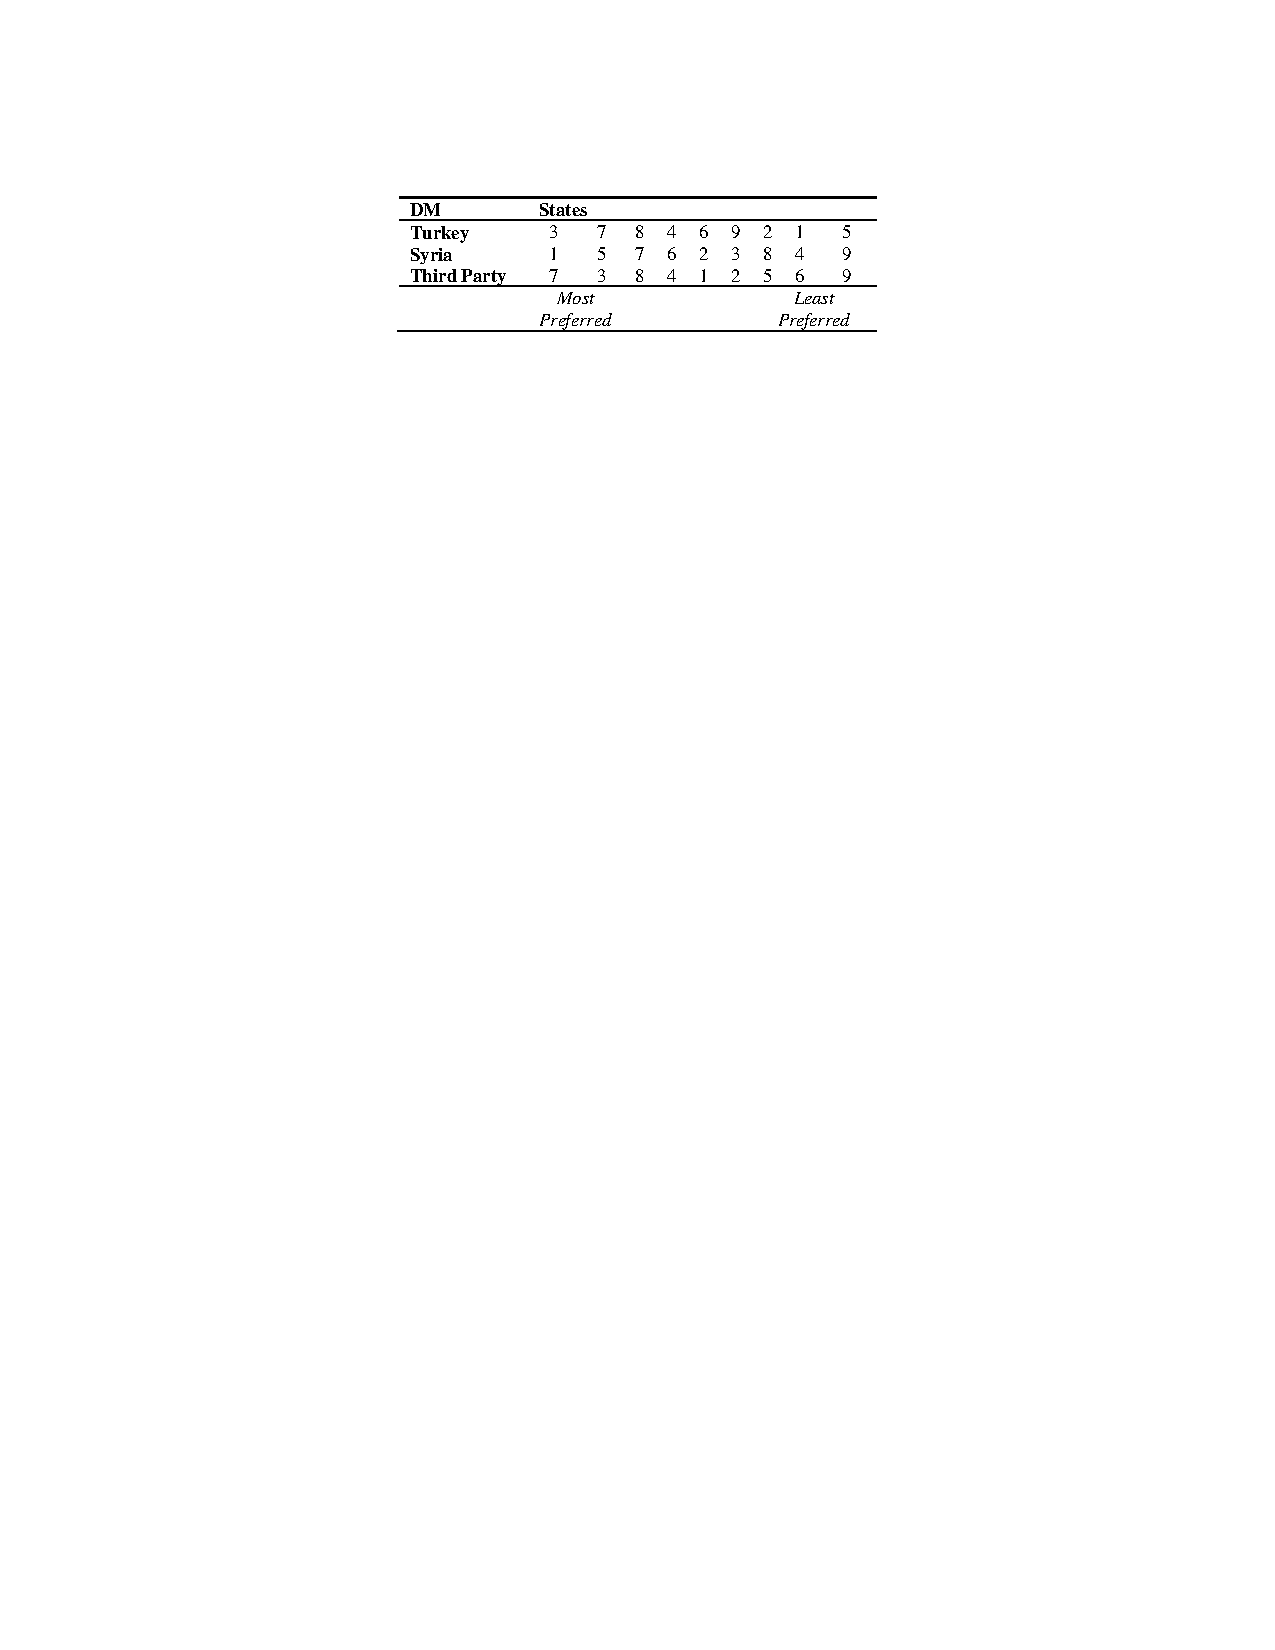
\includegraphics[scale=1]{PDF-IMG/tables/14.pdf}

\caption{Ranking of states for DMs in the 1998 conflict with the third party}

\label{tbl:t14}
\end{table}

\begin{table}[H]
\centering
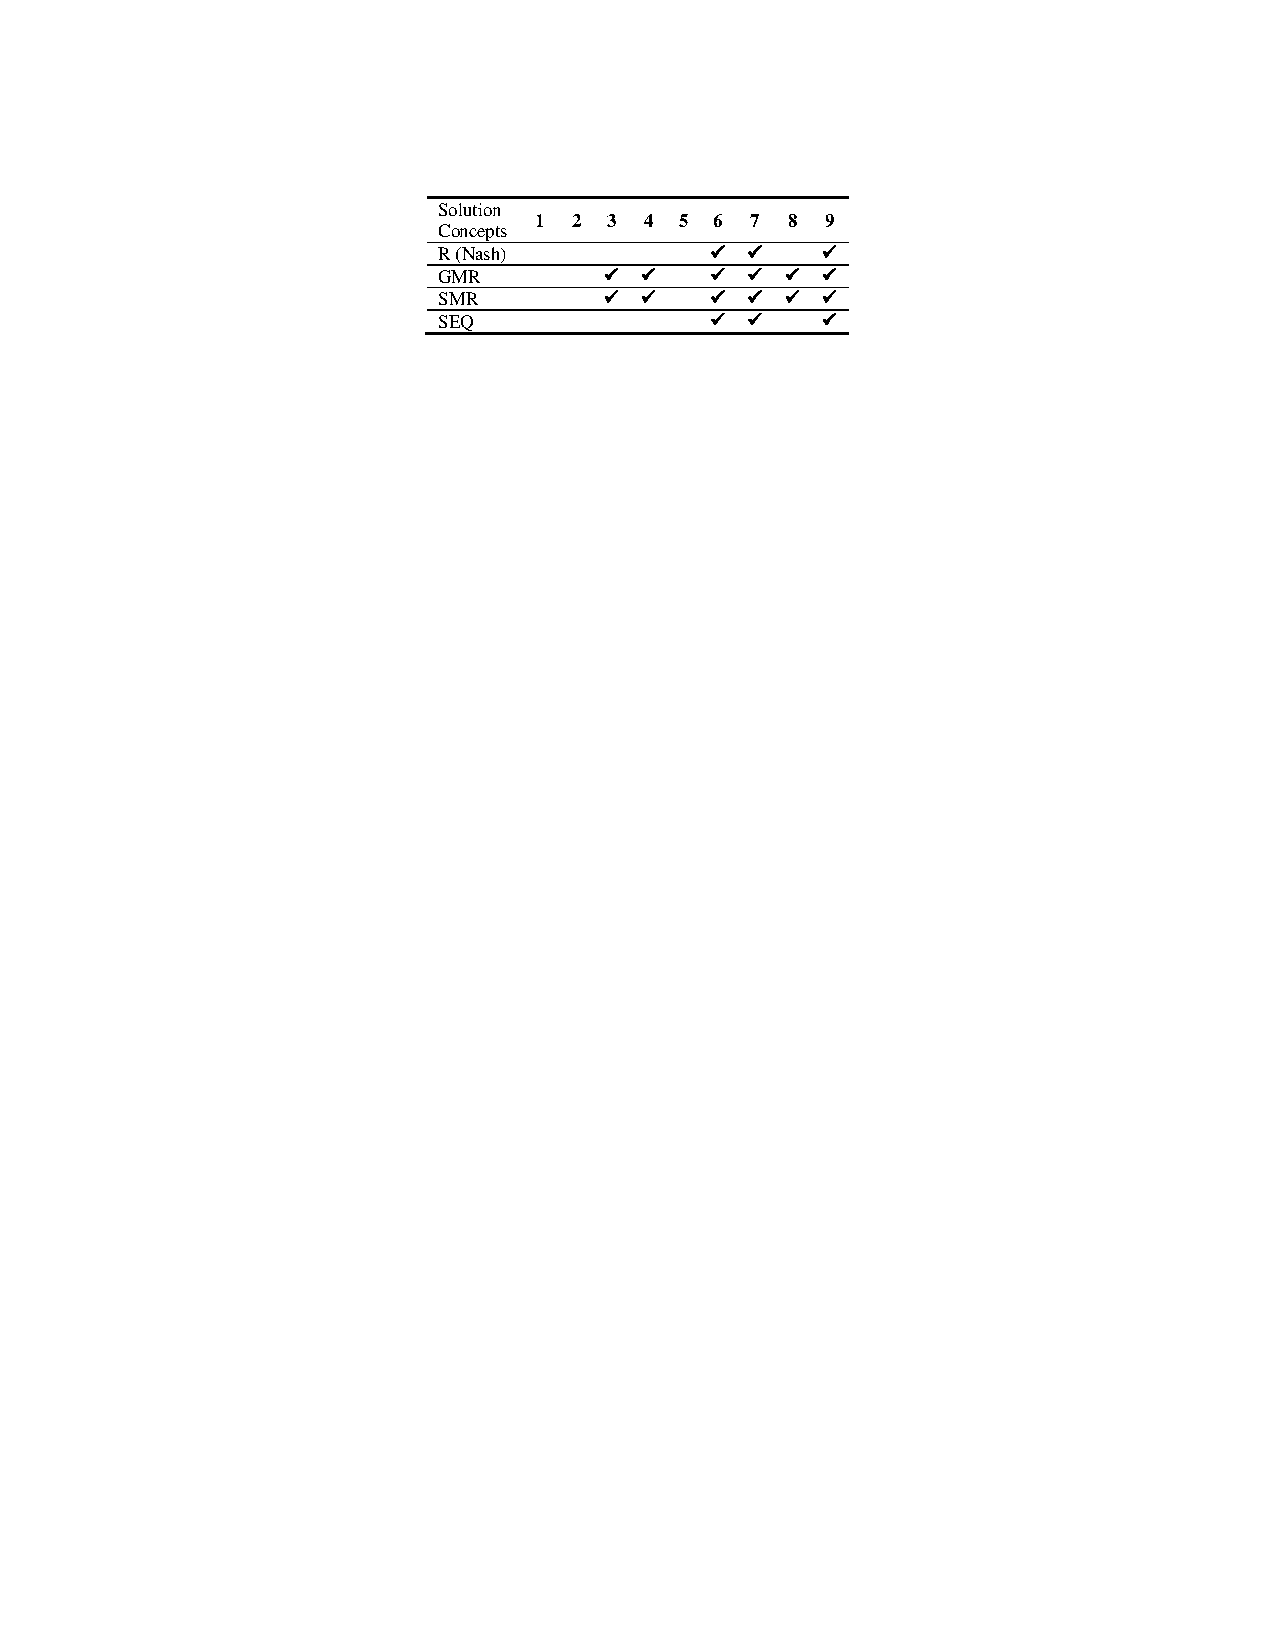
\includegraphics[scale=1]{PDF-IMG/tables/15.pdf}

\caption{Equilibrium results for the 1998 conflict with the third party}

\label{tbl:t15}
\end{table}

This conflict study shows that Turkey played a more important role than Syria and did not have to use water as a weapon. Moreover, Turkey's superior military power puts it at an advantage, which allowed it to threaten Syria with an invasion, thereby bringing the game to an end. The strongest equilibrium states are 6 and 9 (Table \ref{tbl:t15}) in which both Syria and Turkey escalate the situation and Turkey invades eventually if the third party does not act. However, with the mediation of the third party, a new equilibrium came about: state 7 in which the third party acts and Syria bans the PKK. As will be explained in the final section, Syria has been put in a Pareto-inferior situation as it had to give up other things in addition to banning the PKK.
The notion of classifying the role of the third party into Arbitrator, Coordinator, and Donor can determine, in advance, how a third party can influence and bring about a potential resolution to the conflict. Table \ref{tbl:t16} shows the actual historical evolution of the 1998 conflict. 


\begin{table}[H]
\centering
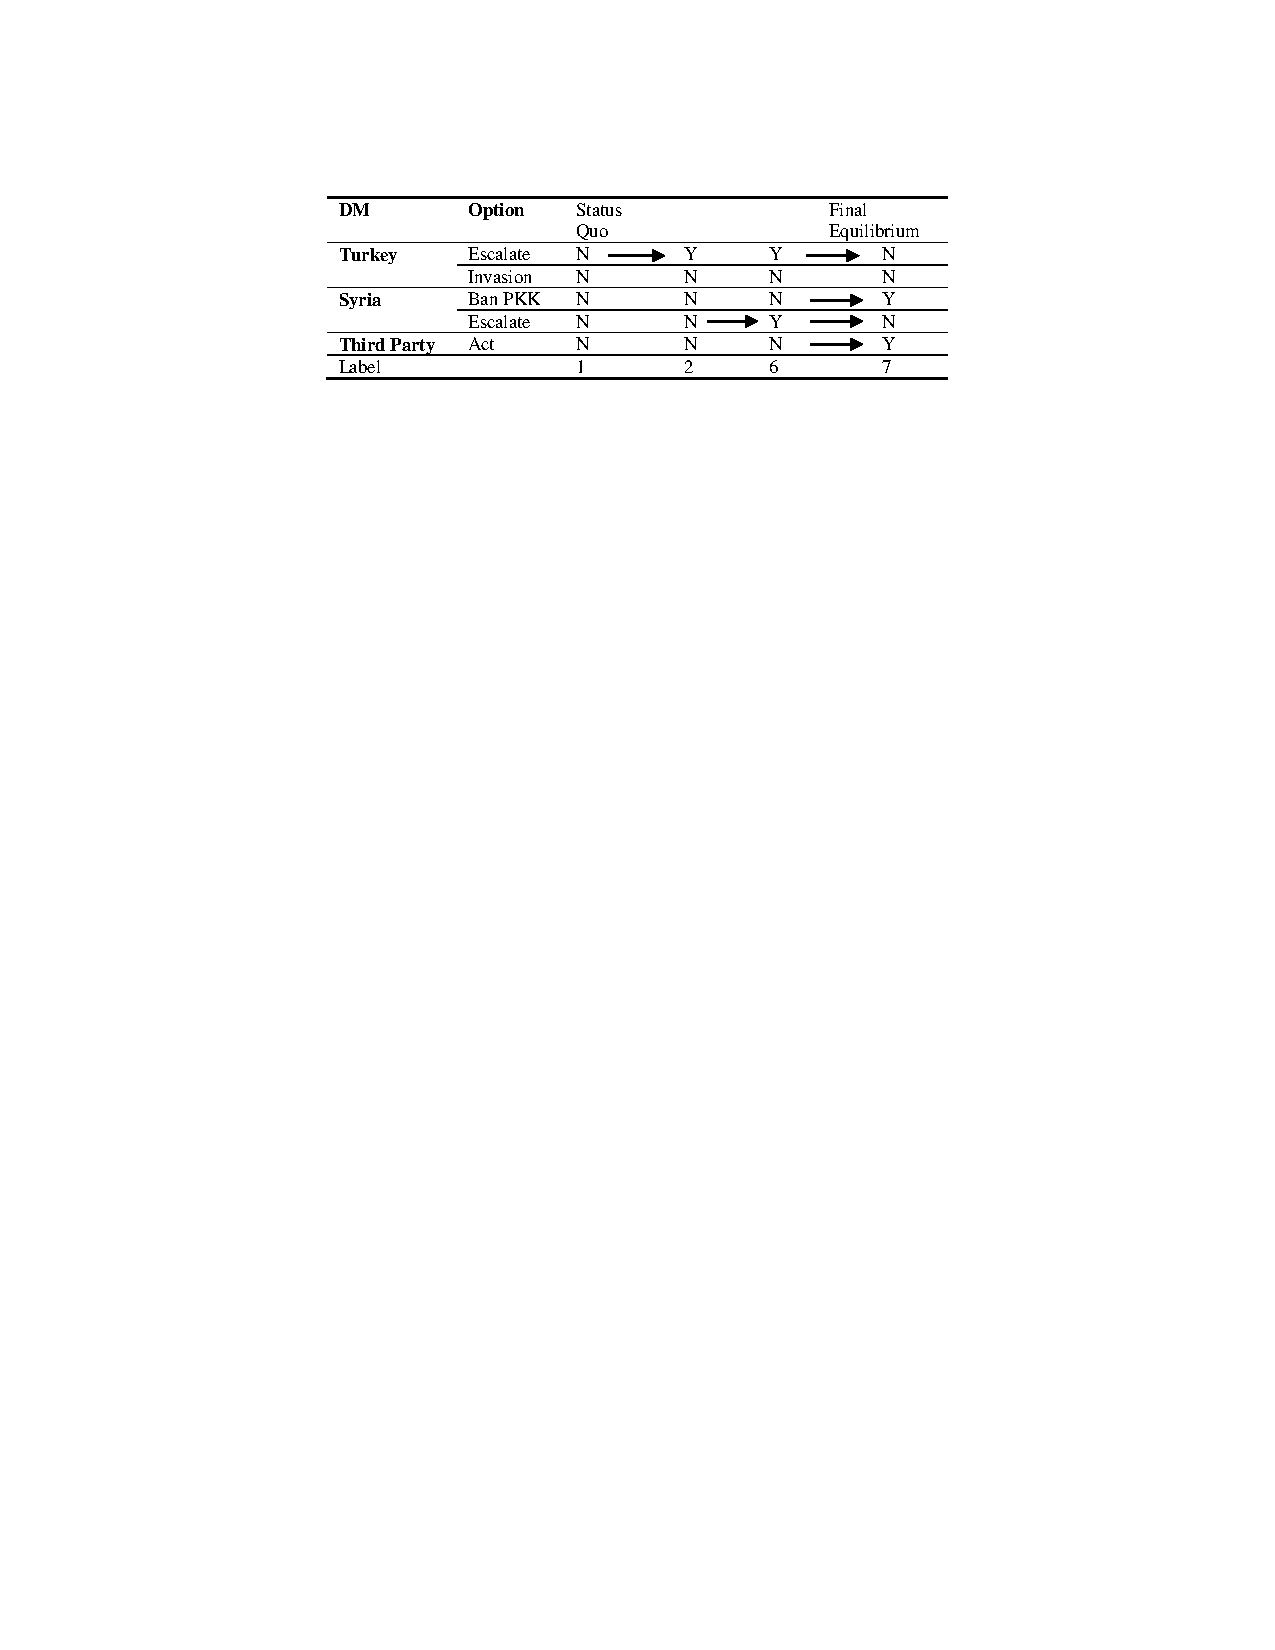
\includegraphics[scale=1]{PDF-IMG/tables/16.pdf}

\caption{Historical evolution of the 1998 conflict}

\label{tbl:t16}
\end{table}

\section{Fundamental Insights}
The analyses confirm similar conclusions drawn by \citet{priscoli2009managing} in their studies of Middle East water conflicts. Firstly, unilateral development of water resources without the coordination and cooperation of other countries sharing the same water recourse may create conflict. Secondly, if one riparian country holds the geographical and military power, unbiased agreements are difficult to achieve. For example, Turkey is upstream and most of the water originates in its territory. Moreover, it has the most advanced military power \citep{priscoli2009managing}, giving it the upper hand in negotiations. As a consequence, Syria ended up in a Pareto-inferior situation because it did not ban the PKK earlier in the conflict which led to the signing of the Adana Agreement. The terms of the agreement include more things Syria has to give up in addition to banning PKK. For instance, Syria accepted Turkish rule over Hatay province, a long disputed land between the two countries. Syria publicly recognized Hatay as a Turkish territory after the Adana agreement, thereby losing two of its playing cards. The third lesson that can be garnered from the case in this paper is the vital role of third party intervention in resolving conflicts.

For the analysis part, the presented conflicts, especially the conflicts in both 1990 and 1998, can be seen as a single evolving conflict. This can serve as a base for methodology development. In addition, a more in-depth analysis could be carried out by mixing various approaches to conflict analysis. For instance, one can carry out hypergame analysis and coalition analysis at the same time for the 1990 conflict.

It is clear that the conflict along the Euphrates River is indeed a complex one. Bilateral and tripartite negotiations continue with mixed success. However, no solid agreement to date has been reached. This paper forms a strong base for carrying out an in-depth analysis of the present situation and determining how the conflict could evolve and what resolution could result in the future. 

%======================================================================

\section{Chapter Summary}

\chapter{Modeling Negotiations in Conflict Resolution Using Inverse GMCR}
%%%%%%%%%%%%%%%%%%%%%%%%%%%%%%%%%%%%%%


Although having a tool such as GMCR to predict and assess equilibria is important, real life conflicts require more than that.  Studies show that 70 percent of all international conflicts since 1945 have involved third party intervention \cite{bercovitch2006}. These interventions strive to change the course of the conflict and ultimately reach a more desired resolution. The available models, including the standard GMCR, only predict the likely outcomes of the conflict. The many extensions of GMCR developed over the years aim to improve how GMCR predicts these outcomes. Another downside of the standard GMCR is the difficulty and subjectivity of the preference rankings of DMs in the conflict. Many GMCR extensions to enrich the preference ranking procedure have been developed, such as strength of preference \cite{hamouda2004strength,hamouda2006strength}, preference uncertainty \cite{li2004}, and fuzzy preferences \cite{bashar2012fuzzy,hipel2011fuzzy}.

In order to address the aforementioned shortcomings, an inverse GMCR is developed here. A main feature of this methodology is that it does not require preference information to model the conflict. This methodology can be utilized in many different  ways. For instance, an intervener can use it to understand how to influence one or more of the disputants in a conflict. On the other hand, one of the disputants can  utilize it to his advantage by understanding how competing parties could behave in order to achieve a desired resolution.

In addition to its use as a negotiation tool, inverse GMCR also can determine a more reliable prediction based on minimal preference ranking information. In GMCR, an analyst is usually confident about the most and least preferred states. The dilemma usually arises with preference rankings between these. Having a methodology such as inverse GMCR allows for exploration of all possible scenarios for unknown preference ranking ranges.    



Although this paper focuses on inverse GMCR, three areas related to modeling third party intervention in conflicts that will be investigated, are as follows:
\begin{enumerate}
\item Inverse approach to conflict resolution (Inverse GMCR): A modeling technique that permits mediators to choose a desired outcome as an equilibrium, and works backwards to achieve it.
\item Inverse status quo analysis: An extension to the previous area that determines whether the desired equilibrium is reachable from the original state.
\item Third party strategy recommendations: A tool to analyze conflicts inviting mediation and furnish insights as to the particular role a mediator should play to resolve the conflict.

\end{enumerate}

%%%%%%%%%%%%%%%%%%%%%%%%%%%

\section{Overview and Objective of Inverse GMCR}

The Graph Model for Conflict Resolution (GMCR) forms an ideal framework to model and analyze conflicts; however, there are challenges to its applicability, especially in estimating the relative preferences of DMs involved in the conflict. In order to address this problem, inverse GMCR allows the analyst to determine how a desired resolution to the conflict can arise by generating all possible relative preferences that achieve it.

The premise of inverse GMCR is that the mediator needs a negotiation tool to influence the DMs. To be valuable, this tool should contain information about what motivates each party to undertake the selection of options leading to the resolution desired by the mediator. Therefore, mediators can focus their resources and strategies to guide the parties toward preferences that lead to this resolution. This tool is not just useful to third parties; stakeholders may be able to take advantage of it to influence their opponent(s).

The current GMCR framework, which forms the basis for inverse GMCR, requires preference ranking information that may not be easy to obtain. Inverse GMCR introduces a modeling approach that requires minimal ordinal preference ranking information up front. A desired resolution, or equilibrium, is decided and a list of preference ranking information leading to the resolution is generated. Thus, inverse GMCR utilizes GMCR as a negotiation tool rather than a prediction tool.

The main objectives of inverse GMCR are the following:
\begin{itemize}
\item Allow a third party to determine a desired resolution and understand how to achieve it
\item Produce strategic information that will help mediators to influence the DMs involved in the conflict
\item Give a range of preference rankings that measures the robustness of the conflict resolution
\end{itemize}

\noindent In contrast, the current GMCR methodology informs the user only about the possible resolution of a conflict based on the input preferences. Inverse GMCR explains how this resolution can be reached. Although the development of this approach was motivated by the need to facilitate third party intervention, other DMs involved in the conflict can also use it. Thus, it will allow for strategic negotiation based on tactical information to achieve a desired outcome.




\section{Procedure and Implementation}

The main difference between inverse GMCR and the standard GMCR procedure is in the order of steps. Figure \ref{fig:procedure_or} illustrates the current procedure for applying GMCR in the real world. A modified version, shown in Figure \ref{fig:procedure_inv}, illustrates how to apply inverse GMCR. The original procedure requires the following inputs for the conflict to be analyzed \cite{Fang1989,fang1993}:
\begin{itemize}
\item Decision makers (DMs)
\item Options for each DM
\item Infeasible states (such as mutually exclusive situations)
\item Allowable transitions
\item Relative preferences
\end{itemize}

\noindent On the other hand, inverse GMCR does not require the ranking of states for all DMs. Its requirements are:
\begin{itemize}
\item Decision makers (DMs)
\item Options for each DM
\item Infeasible states (such as mutually exclusive situations)
\item Allowable transitions
\item Desired resolution
\end{itemize}
\noindent The result will be a list of possible state rankings that will make the desired resolution stable under the selected stability definition.


\begin{center}
\begin{figure}
\centering
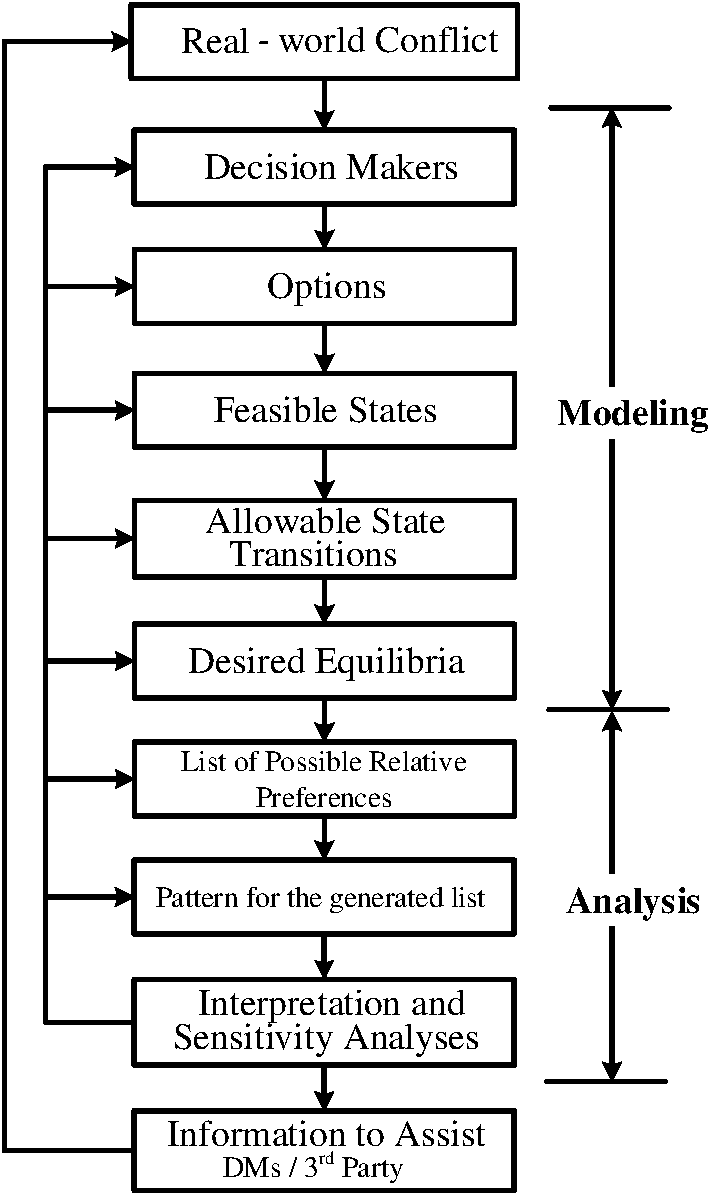
\includegraphics[scale=0.55]{PDF-IMG/GMCR_inv.pdf}

\caption{Inverse GMCR procedure in a real world conflict (modified from \cite{fang1993})}

\label{fig:procedure_inv}
\end{figure}
\end{center}


In order to formally define the \textit{inverse approach to GMCR}, one needs to furnish some definitions and notation. First, we show how a DM's preferences can be represented using an ordinal payoff vector. 

\begin{definition}
\label{def:ord_pref}
\rm
The ordinal payoff vector of DM $i$, denoted by $P_i$, is
$$p^i=P_i=(p_1^i,p_2^i, \dots ,p_m^i ) , \quad P_i \in \mathbb{R}^m  $$

\end{definition}

\noindent If $s_a,s_b \in S$, then DM $i$ prefers $s_a$ to $s_b$ or is indifferent ($s_a \succsim_i s_b$) \emph{iff} $p_a^i \geq p_b^i$. An equivalent notation is $$P_i(s_j)=p_j^i$$ so that $s_a\succsim_i s_b$ \emph{iff} $P_i(s_a)\geq P_i(s_b)$

For example, if $P_i=(5,0,6,2,6)$ then the ordinal payoff value for DM $i$ for state 1 is equal to 5. Thus, $P_i(s_1)=5,P_i(s_2)=0,P_i(s_3)=6,P_i(s_4)=2,$ and $P_i(s_5)=6$. Because preferences are assumed to be transitive, the payoff vector can be translated into a preference profile. A preference ranking for DM $i$ is a list of feasible states ordered from most to least preferred for DM $i$, where ties are allowed. %Equally preferred states are marked with a bar or a parenthesis in the preference ranking.
In the previous example, the preference ranking for DM $i$ would be $PR_i=s_3 \sim s_5 \succ s_1 \succ s_4 \succ s_2$.

Note that the same preference ranking can be represented by many different ordinal payoff vectors. Two such ordinal payoff vectors are called \emph{equivalent}.

\begin{comment}

\begin{definition}
\rm

Let $N=\{1,2,\dots,n\}$ represent the set of DMs, $S=\{s_1, s_2, \dots, s_m\}$ represent the set of feasible states in a graph model. If $s_a\succsim s_b \succsim \dots \succsim s_z$, then $PR_i=\{s_a, s_b, \dots, s_z\} $ is a preference ranking.

%and $P_i=(p_1^i,p_2^i, \dots ,p_m^i ) , \quad P_i \in \mathbb{R}^m  $ be the ordinal payoff vector of DM $i$. The preference profile for DM $i$ denoted by $PP_i$, is given by:

%where $a,b,\dots ,z \in \mathbb{N}=\{1,2,\dots ,m\} $ and $P_i(s_a)\succsim P_i(s_b)\succsim \dots \succsim P_i(s_z)$
\end{definition}

\end{comment}


\begin{definition}
\rm
If $p^i \in \mathbb{R}^m$ is an ordinal payoff vector for DM $i \in N$, then $(p^1,p^2,\dots ,p^n) \in \mathbb{R}^{mn}$ is a preference profile.

\end{definition}


Inverse GMCR will be defined using both ordinal payoff vectors and preference profiles. In the graph model, analysis means finding all equilibria given a preference profile. In inverse GMCR, the problem is to find all preference profiles under which a given state is an equilibrium with respect to a selected stability definition.  After the introduction of preference profiles, a graph model can be denoted $G=\langle N,S,P\rangle$ where $N$ is the list of DMs $N=\{1,\dots ,n\}$, $S$ is the set of feasible states $S=\{s_1, s_2, ..., s_m\}$, and $P$ is the preference profile $P \in \mathbb{R}^{mn}$.


The \emph{inverse problem} for a desired equilibrium state $s_E \in S$ is to find all $p \in \mathbb{R}^{mn}$ such that state $s_E$ is stable for all DMs if the preference profile is $p$.


\noindent \textbf{Inverse Nash problem for $s_E$:} Find $p \in \mathbb{R}^{mn}$ such that $s_E \in Nash(G)$ where $G=\langle N,S,P\rangle $

\noindent \textbf{Inverse SEQ problem for $s_E$:} Find $p \in \mathbb{R}^{mn}$ such that $s_E \in SEQ(G)$ where $G=\langle N,S,P\rangle $

\noindent \textbf{Inverse GMR problem for $s_E$:} Find $p \in \mathbb{R}^{mn}$ such that $s_E \in GMR(G)$ where $G=\langle N,S,P\rangle $

\noindent \textbf{Inverse SMR problem for $s_E$:} Find $p \in \mathbb{R}^{mn}$ such that $s_E \in SMR(G)$ where $G=\langle N,S,P\rangle $

A more formal definition according to each solution concept will follow.


\subsection{Algorithms}

In order to implement inverse GMCR, two approaches were investigated. The first was the brute-force method. As the name suggests, this method tests each possible preference profile for each DM against the desired equilibrium. Since the number of possible preference rankings is fairly large, a decision support system was designed to test the concept. The number of iterations required for a model, assuming strict ordinal preferences, is given by $(m!)^{n}$ where $m$ is the number of feasible states and $n$ is the number of DMs.  If the combination of preference vectors for all DMs (i.e. preference profile) achieves the desired equilibrium, it will be saved into a list. The second algorithm was designed after observing the pattern produced by the brute-force method. It was clear that results followed certain rules which can be defined more formally, as outlined in the following subsections. %The pseudo-codes for both algorithms will be given in the decision support system section below.%



\subsection{Inverse Nash Equilibrium}
\begin{definition}
\rm
\label{def:nash_inv1}
State $s_E$ is a Nash equilibrium \emph{iff} $p_i(s)\leq p_i(s_E)$ for all $i \in N$ and all $s \in R_i(s_E)$


%all states $s_(m-E) \in R^{+}_{n}(s)$ for all $n \in N$ must satisfy  $q <_{N} s$ in all $P_{N}$
\end{definition}

%\begin{theorem}
%\rm
%\label{thm:nash_inv2}

%If all states $q \in R^{+}_{n}(s)$ satisfy $q <_{n} s$ for all $n \in N$, then state $s$ is Nash stable.
%\end{theorem}

Thus, inverse GMCR should produce all preference profiles that make the desired state $s_E$ a Nash equilibrium. For illustration, inverse GMCR list according to preference profiles (or payoff vectors), denoted by $IPV(s_E)$, is shown in Fig \ref{fig:IPVil}. Note that each of the $T$ rows is a preference profile, a combination of ordinal payoff vectors, that will make state $s_E$ stable for all DMs. The possible number of profiles is denoted by $T$. %Similarly, inverse GMCR list according to preference rankings, denoted by $IPR(s_E)$, is shown.

\begin{center}
\begin{figure*}
\centering


$IPV(s_E)= \begin{Bmatrix}
[^1p_1^1,^1p_2^1, \dots ,^1p_m^1 ] & [^1p_1^2,^1p_2^2, \dots ,^1p_m^2 ] & \dots & [^1p_1^n,^1p_2^n, \dots ,^1p_m^n ] \\ 
[^2p_1^1,^2p_2^1, \dots ,^2p_m^1 ] & [^2p_1^2,^2p_2^2, \dots ,^2p_m^2 ] & \dots & [^2p_1^n,^2p_2^n, \dots ,^2p_m^n ] \\ 
\vdots  & \vdots  & \ddots  & \vdots \\ 
[^Tp_1^1,^Tp_2^1, \dots ,^Tp_m^1 ] & [^Tp_1^2,^Tp_2^2, \dots ,^Tp_m^2 ] & \dots & [^Tp_1^n,^Tp_2^n, \dots ,^Tp_m^n ]
\end{Bmatrix} $


\caption{Representation of the inverse preference profiles list for state $s_E$}

\label{fig:IPVil}
\end{figure*}
\end{center}

\noindent Note that $^hp_j^i$ is player $i$'s ordinal payoff for state $j$ in profile $h$.

\begin{definition}
\rm
A \emph{Nash $IPV(s_E)$} is a list of preference profiles, $p \in \mathbb{R}^{mn}$, where in each profile, for all $i \in N$, all $q \in R^{+}_{i}(s_E)$ satisfies $P_i(q)\leq P_i(s_E)$.
\end{definition}

\subsection{Inverse SEQ Equilibrium}

\begin{definition}
\rm
\label{def:seq_inv}
An \emph{SEQ $IPV(s_E)$} is a list of preference profiles, $p \in \mathbb{R}^{mn}$, such that for each state $q \in R^{+}_{i}(s_E)$ in the preference profile, there exists at least one state $k\in R^{+}_{N-i}(q)$ satisfying $P_i(k)\leq P_i(s_E)$ for all %$q \in  R^{+}_{i}(s_E)$ and all 
$i \in N$ 
\end{definition}

In other words, the combination of payoff vectors must ensure that for each UI a DM can take, there exists at least one sanction that will put the original player in a less preferred state. Please note that the notation $N-i$ means all DMs other than $i$.

%\begin{definition}
%\rm
%An \emph{SEQ IPR(S)} is a combination of $P_{N}$ such that, for all UI states $s_{1} \in R^{+}_{i}(s)$, there exist at least one $q \in R_{N-i}^{+}(s_{1})<_{i} s$ for all $i \in N$
%\end{definition}


\subsection{Inverse GMR Equilibrium}

\begin{definition}
\label{def:gmr_inv}
\rm
A \emph{GMR $IPV(s_E)$} is a list of preference profiles, $p \in \mathbb{R}^{mn}$, such that for each state $q \in R^{+}_{i}(s_E)$ in the preference profile, there exists at least one state $k\in R_{N-i}(q)$ satisfying $P_i(k)\leq P_i(s_E)$ for all %$q \in  R^{+}_{i}(s_E)$ and all 
$i \in N$ 
\end{definition}

%\begin{definition}
%\rm
%\label{def:gmr_inv}
%A \emph{GMR IPR(S)} is a combination of $P_{N}$ such that, for all UI states $s_{1} \in R^{+}_{i}(s)$, there exist at least one $q \in R_{N-i}(s_{1})<_{i} s$ for all $i \in N$
%\end{definition}

\subsection{Inverse SMR Equilibrium}

\begin{definition}
\label{def:smr_inv}
\rm
An \emph{SMR $IPV(s_E)$} is a list of preference profiles, $p \in \mathbb{R}^{mn}$, such that for each state $q \in R^{+}_{i}(s_E)$ in the preference profile, there exists at least one state $k\in R_{N-i}(q)$ satisfying $P_i(k)\leq P_i(s_E)$ and all $h \in R_{i}(k)$ satisfy $P_i(h)\leq P_i(s_E)$ for all %$q \in  R^{+}_{i}(s_E)$ and all %
$i \in N$ 
\end{definition}

%\begin{definition}
%\label{def:smr_inv}
%\rm
%An \emph{SMR IPR(S)} is a combination of $P_{N}$ such that, for all UI states $s_{1} \in R^{+}_{i}(s)$, there exist at least one $q \in R_{N-i}(s_{1})<_{i} s$ for all $i \in N$ and all $k \in R_{i}(q)<_{i} s$ for all $i \in N$
%\end{definition}

\section{Inverse Status Quo Analysis}
Every real world conflict has a starting point from which the conflict evolves. This point or state is called \emph{status quo} \cite{fang1993}. Depending on the status quo, a potential equilibrium may or may not be reached. 

Li et al. developed algorithms and formal definitions to inspect the attainability of a potential resolution (\emph{equilibrium}) from a certain state (\emph{status quo}) \cite{li2004squo,li2005squo}. An inverse approach to determine the required starting points in order to attain a desired equilibria is achieved by tracking the evolution of the conflict backward from a desired equilibrium to the status quo states.

\section{Third Party Strategy Recommendations}
Various third party roles and strategies are investigated and presented in another paper by the authors \cite{rami2012smc} . Several methodologies are developed to determine the best role and strategy a mediator should undertake in any particular conflict situation. The motivation to introduce such a methodology is to operationalize the notion of third party intervention.


%%%%%%%%%%%%%%%%%%%%%%%%%%%%%

\section{Decision Support System}

The introduction of inverse GMCR makes the need for a decision support system obvious. Solving problems by hand is possible but tiresome, time consuming, and error-prone. First, a code to test each preference profile was developed. This is called the Brute-Force method.

The matrix approach to GMCR allows for faster processing \citep{Xu2009Jr}. The last decision support system, GMCR II, was developed by Xiaoyong (John) Peng in 1999 \citep{peng1999decision,fang2003a,fang2003b}. Until recently, no significant update was made to the decision support system, even though the program had issues that sometimes caused it to crash or display error messages.

A project to combine both the logical and matrix approaches into a robust and flexible decision support system was initiated by Rami Kinsara and Oskar Petersons. The objective of this system was to overcome the limitations of the previous version and also add new extensions and capabilities that it did not support. A main objective of the new system is to include the inverse GMCR methodology. Chapter \ref{sec:DSS+} discusses in detail all aspects of the new DSS.

\section{Application}
\subsection{Standard GMCR Results}
The water conflict between Syria and Iraq in 1975 is explained in Section \ref{Conflict1975}. In order to illustrate the inverse GMCR, this conflict will be re-investigated. 

The standard GMCR analysis for this conflict is provided in detail in Section \ref{Conflict1975Analysis}. As mentioned earlies in this research, standard GMCR requires preference information (or ranking of states). Since this model is fairly small, it is not difficult to derive the preference information from the conflict background, although it remains subjective. The ranking of states for this conflict is shown in Table \ref{tbl:t5}. Running the GMCR standard analysis predicts the most likely outcome in terms of equilibria based on the input preferences. Table \ref{tbl:t8} shows the equilibrium results according to different behavior patterns. Nash and Sequential Stability (SEQ) are the strongest stability definitions, meaning that DMs are not motivated to deviate from a particular state if the conflict reaches it. General Metarationality (GMR) and Symmetric Metarationality (SMR) are not as strong. More formal definitions and the relationships among the different stability definitions are mentioned earlier and can be found in \cite{Fang1989}.

The objective of the standard GMCR analysis is to determine the equilibrium states, the states from which no DM is motivated to move. Therefore, once an equilibrium is attained, the conflict will probably end there. As mentioned in the historical background, the conflict reached state 6 in which both Syria and Iraq go to war, a strong equilibrium as shown in Table \ref{tbl:t8}. 

The standard GMCR methodology lacks the ability to determine a more desired resolution and explain how it can be achieved. This example also illustrates the subjectivity in determining the ranking of states. 

\subsection{Inverse GMCR Results}
The goal of any intervention is to bring about a better resolution for all parties to the conflict. Inverse GMCR acts as a negotiation tool allowing the analyst to determine a more desirable resolution. In this particular case, a more desired resolution would be state 2 in which both Syria and Iraq stop escalating and water is released to Iraq. The objective of inverse GMCR is to provide mediators with strategic information in order to help them focus their efforts effectively and efficiently. Here, the mediation aims to influence Syria to release water and stop escalating. Using inverse GMCR, state 2 is chosen as a desired equilibrium and the decision support system was used to run the analysis. The findings indicate that 240 possible preference profiles can achieve the desired resolution. After analyzing these results, two meaningful patterns were identified that lead the conflict to the desired equilibrium:
\begin{itemize}
\item If Syria has state 2 as the most preferred state (Nash Stability)
\item If and only if Syria prefers states 4, 5, or 6 to state 2 (Sequential Stability)
\end{itemize}

\noindent In other words, state 2 will be the resolution to the conflict if and only if (1) Syria prefers not to escalate or (2) being attacked by Iraq is less preferred for Syria. Having this strategic information could be vital to the mediators as they focus their efforts on influencing Syria to change its preference rankings. Consequently, the final outcome of the conflict would change.


\begin{center}
\begin{figure}
\centering
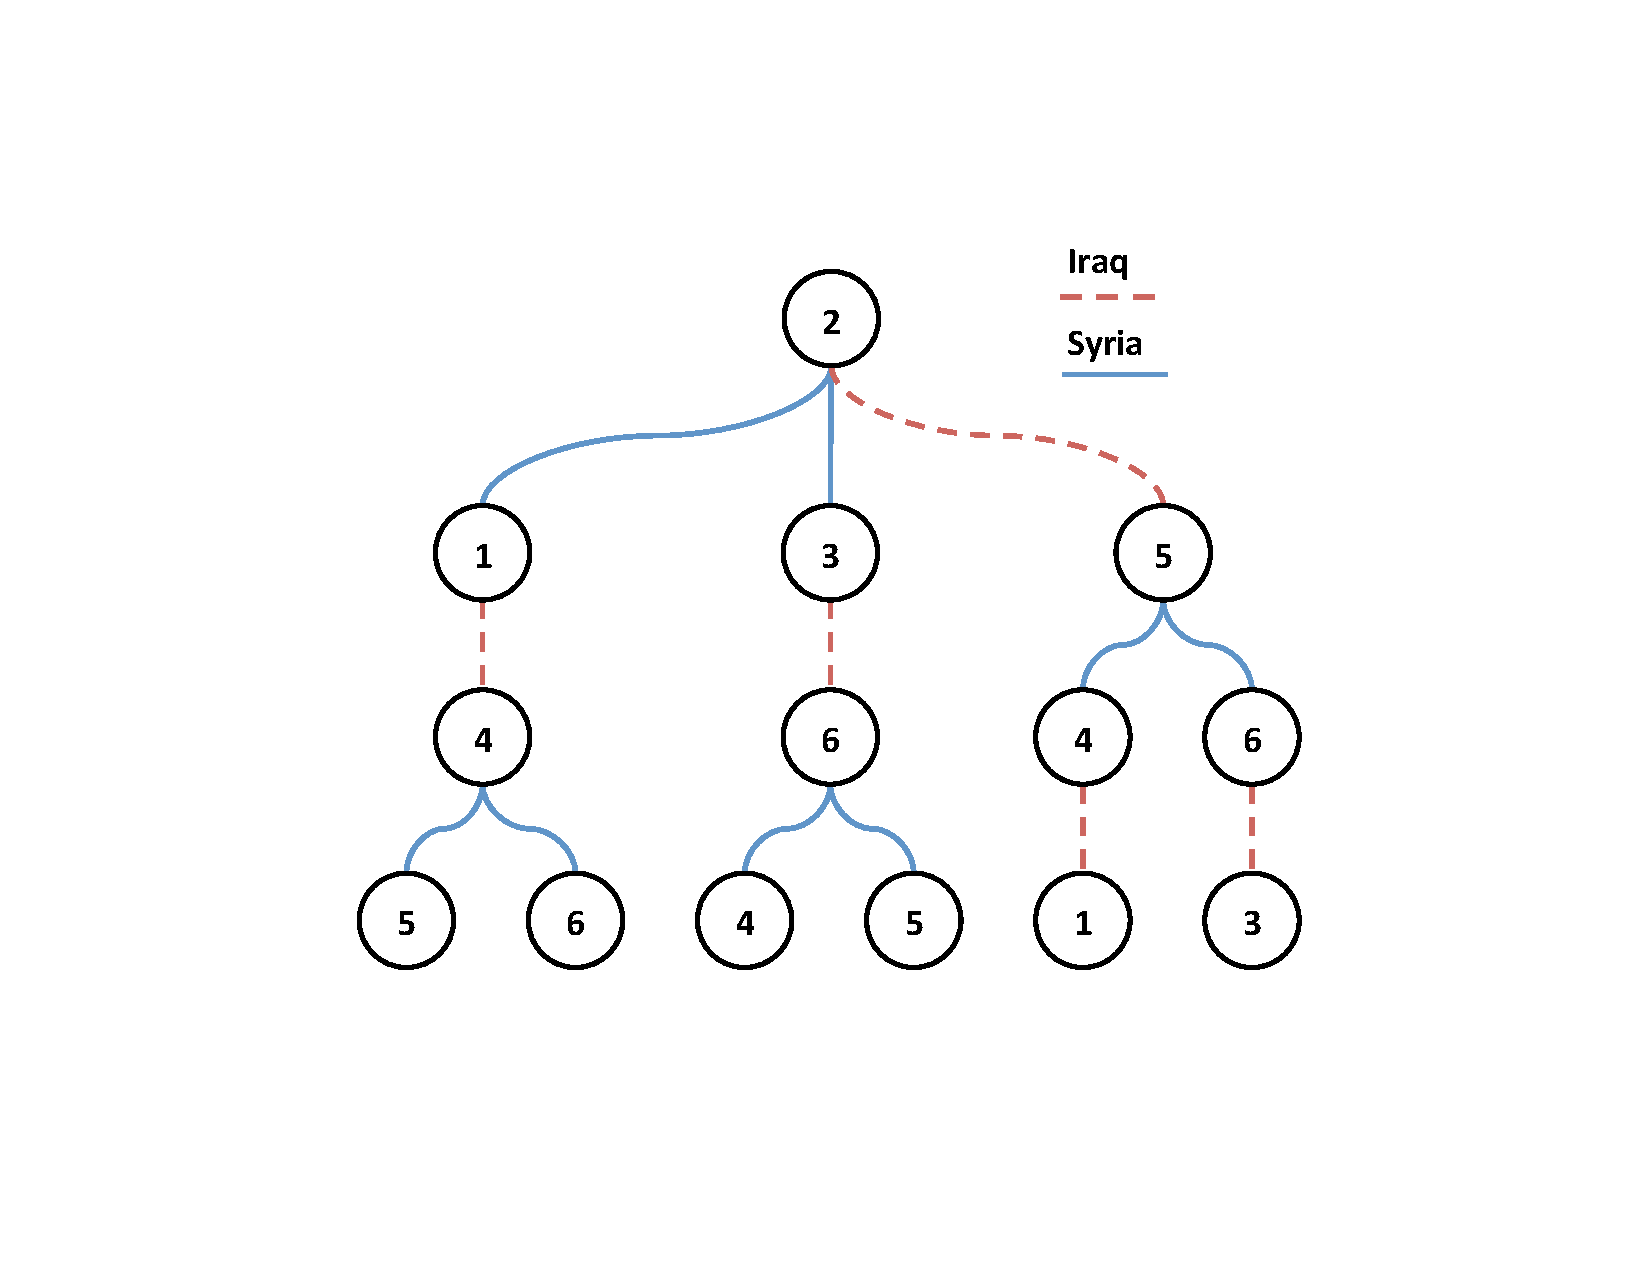
\includegraphics[width=2.5in]{PDF-IMG/graphsq.pdf}

\caption{Inverse Status Quo Diagram for the Syria-Iraq conflict}

\label{fig:graphsq}
\end{figure}
\end{center}

The diagram in Figure \ref{fig:graphsq} illustrates the inverse status quo tree in which state 2 is clearly reachable from state 6. Usually, when all moves in a conflict are reversible, states can be reachable using all DMs level. However, this tool becomes very valuable when irreversible moves are introduced to a conflict. 

% Reminder: the "draftcls" or "draftclsnofoot", not "draft", class option
% should be used if it is desired that the figures are to be displayed while
% in draft mode.


% An example of a floating figure using the graphicx package.
% Note that \label must occur AFTER (or within) \caption.
% For figures, \caption should occur after the \includegraphics.
%
% \begin{figure}
% \centering
% \includegraphics[width=2.5in]{myfigure}
% where an .eps filename suffix will be assumed under latex,
% and a .pdf suffix will be assumed for pdflatex
% \caption{Simulation Results}
% \label{fig_sim}
% \end{figure}


% An example of a double column floating figure using two subfigures.
% (The subfigure.sty package must be loaded for this to work.)
% The subfigure \label commands are set within each subfigure command, the
% \label for the overall fgure must come after \caption.
% \hfil must be used as a separator to get equal spacing
%
% \begin{figure*}
% \centerline{\subfigure[Case I]{\includegraphics[width=2.5in]{subfigcase1}
% where an .eps filename suffix will be assumed under latex,
% and a .pdf suffix will be assumed for pdflatex
% \label{fig_first_case}}
% \hfil
% \subfigure[Case II]{\includegraphics[width=2.5in]{subfigcase2}
% where an .eps filename suffix will be assumed under latex,
% and a .pdf suffix will be assumed for pdflatex
% \label{fig_second_case}}}
% \caption{Simulation results}
% \label{fig_sim}
% \end{figure*}


% An example of a floating table. Note that, for IEEE style tables, the
% \caption command should come BEFORE the table. Table text will default to
% \footnotesize as IEEE normally uses this smaller font for tables.
% The \label must come after \caption as always.
%
% \begin{table}
% increase table row spacing, adjust to taste
% \renewcommand{\arraystretch}{1.3}
% \caption{An Example of a Table}
% \label{table_example}
% \begin{center}
% Some packages, such as MDW tools, offer better commands for making tables
% than the plain LaTeX2e tabular which is used here.
% \begin{tabular}{|c||c|}
% \hline
% One & Two\\
% \hline
% Three & Four\\
% \hline
% \end{tabular}
% \end{center}
% \end{table}


\subsection{Conclusions and Insights}
The historical evolution of the conflict is illustrated in Table \ref{tbl:ACT1975CH5}. Note that state numbers with an asterisk (*) indicate mediation. In inverse GMCR context, a mediator (or Iraq) can influence Syria in two ways:

\begin{itemize}
\item Making the escalation option for Syria less preferred 
\item Making the attack option by Iraq disastrous for Syria
\end{itemize}

\begin{table}[H]
\centering
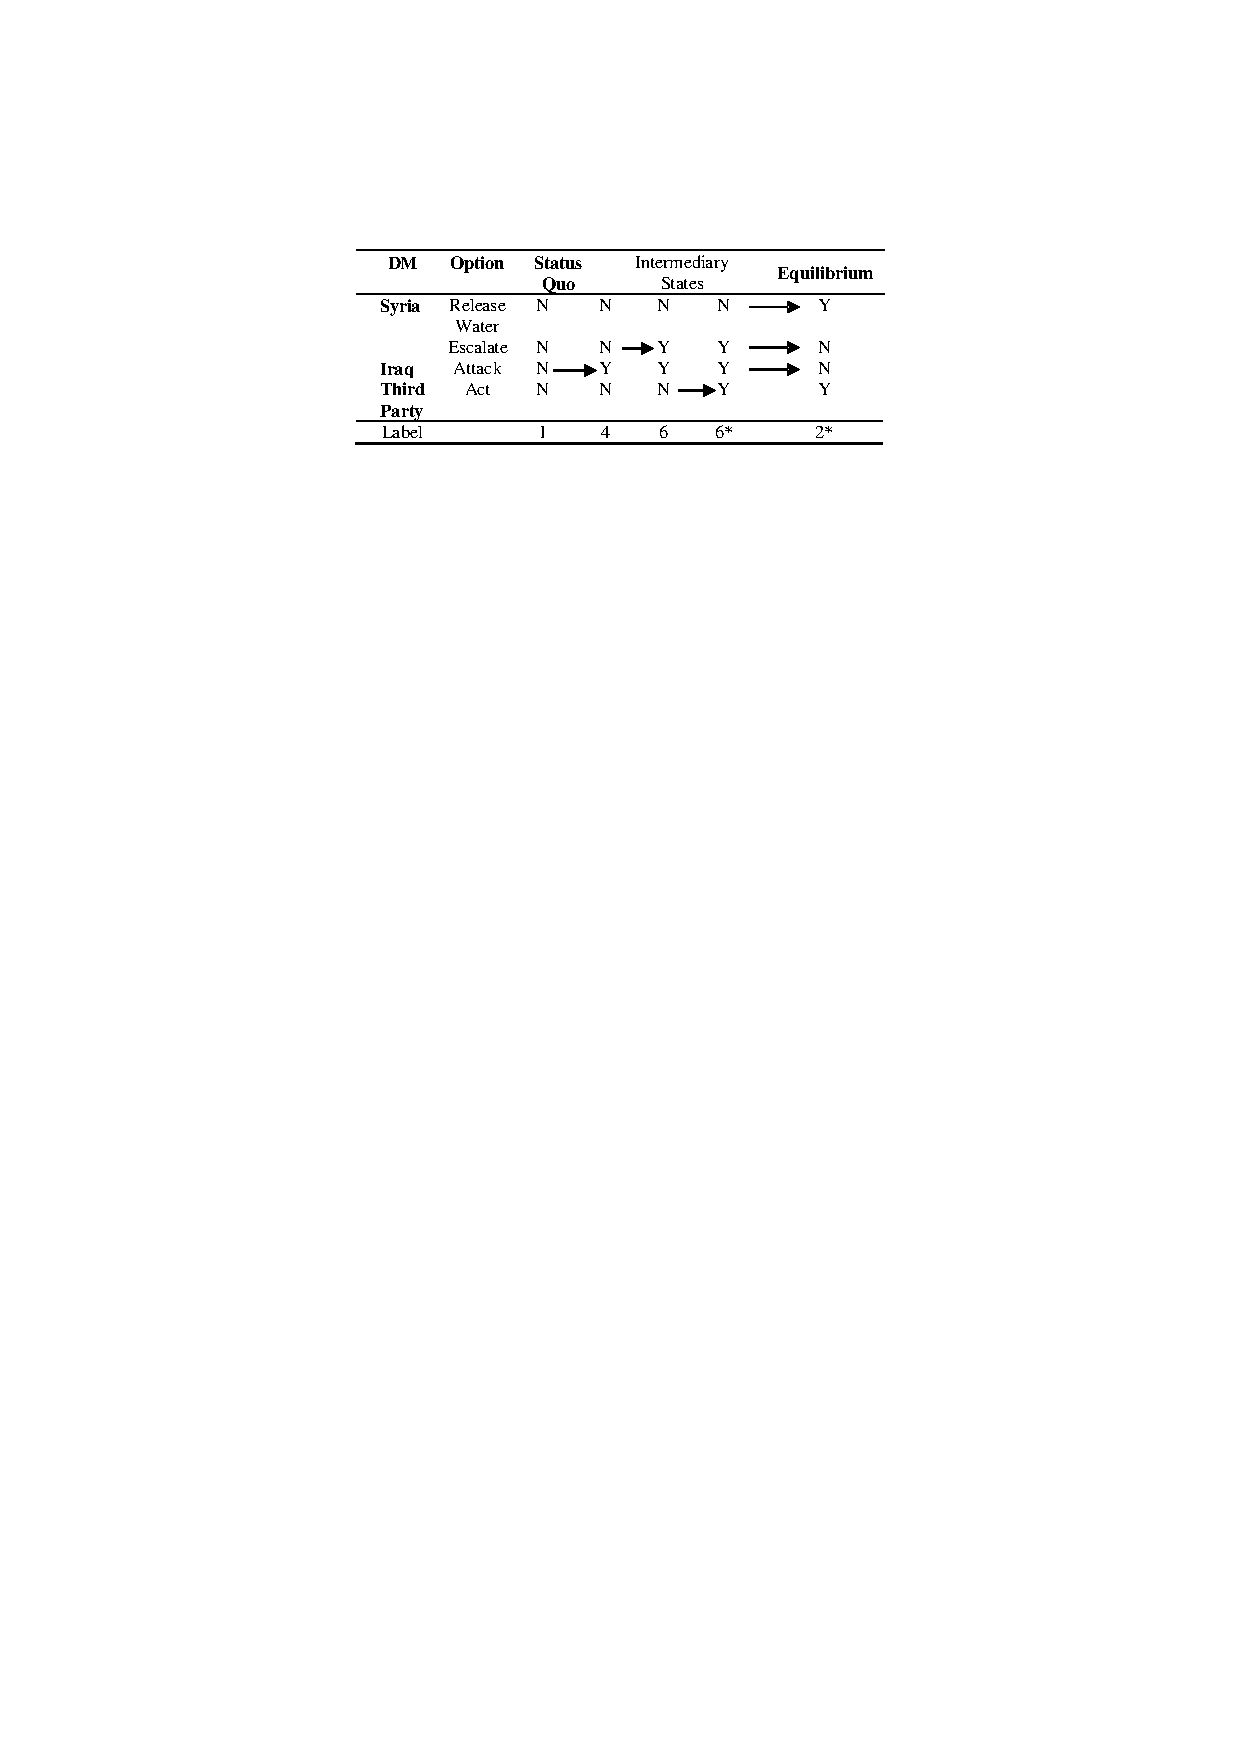
\includegraphics[scale=1]{PDF-IMG/tables/ACT1975CH5.pdf}

\caption{Historical evolution of the 1975 conflict}

\label{tbl:ACT1975CH5}
\end{table}

In this conflict, Saudi Arabia mediated the conflict by contributing to a basin fund that would finance irrigation reform \cite{akanda2007tigris}. Therefore, escalation by Syria became less preferred as it risked losing this fund, in addition to other factors related to international pressure and war costs.

This conflict emphasizes how third party intervention can change the course of the conflict and bring about a better resolution.  Studies show that 70 percent of all international conflicts since 1945 have involved mediation \cite{bercovitch2006}. The strategy of intervention is as important as the intervention itself if not more. Therefore, a tool to provide insights on how to achieve a desired resolution is valuable. Inverse GMCR is a strategic tool that utilizes GMCR as a negotiation tool rather than as a prediction tool. Moreover, its information requirements are minimal.

%%%%%%%%%%%%%%%%%%%%%%%%%%%%%

\section{Chapter Summary}

\chapter{Comprehensive Decision Support System}
\label{sec:DSS+}
The introduction of the inverse approach makes the need for a decision support system obvious. Solving problems by hand is possible but tiresome, time consuming, and error-prone. First, a code to test each preference profile was developed. This is called the Brute-Force method
The matrix approach to GMCR allows for faster processing \citep{xu2007matrix,xu2009}. The last decision support system, GMCR II, was developed by Xiaoyoung (John) Peng back in 1999 \citep{peng1999decision}. Until recently, no significant update was made to the decision support system, even though, the program had issues that sometimes caused it to crash or display error messages.
A project to combine both the logical and matrix approaches into a more robust and flexible decision support system was initiated by Oskar Petersons and Rami Kinsara under the supervision of Prof. Keith Hipel and Prof. D. Marc Kilgour. The objective of this system is to overcome the limitations in the previous version and also add new extensions and capabilities that it did not support. A main objective of the new system is to include the inverse approach methodology. An important feature of the software is the ability to narrate the output results. More extensions and features are planned.

\section{Conflict Specification}
\label{sec:ConfSpecs5}
One of the GMCR+ project's central goals is the creation of a simple and flexible system to model conflicts in an electronic format. In pursuit of this goal, it is required to identify the parameters of the conflict and make logical connections between them. Since the DSS is programmed using an object oriented language, the conflict parameters will be referred to as objects. Figure \ref{fig:confspecs} illustrates the top-level specifications (i.e. objects) of the conflict model in the DSS. In the following subsections, each object is explained and its properties illustrated.

\begin{center}
\begin{figure}[h!]
\centering
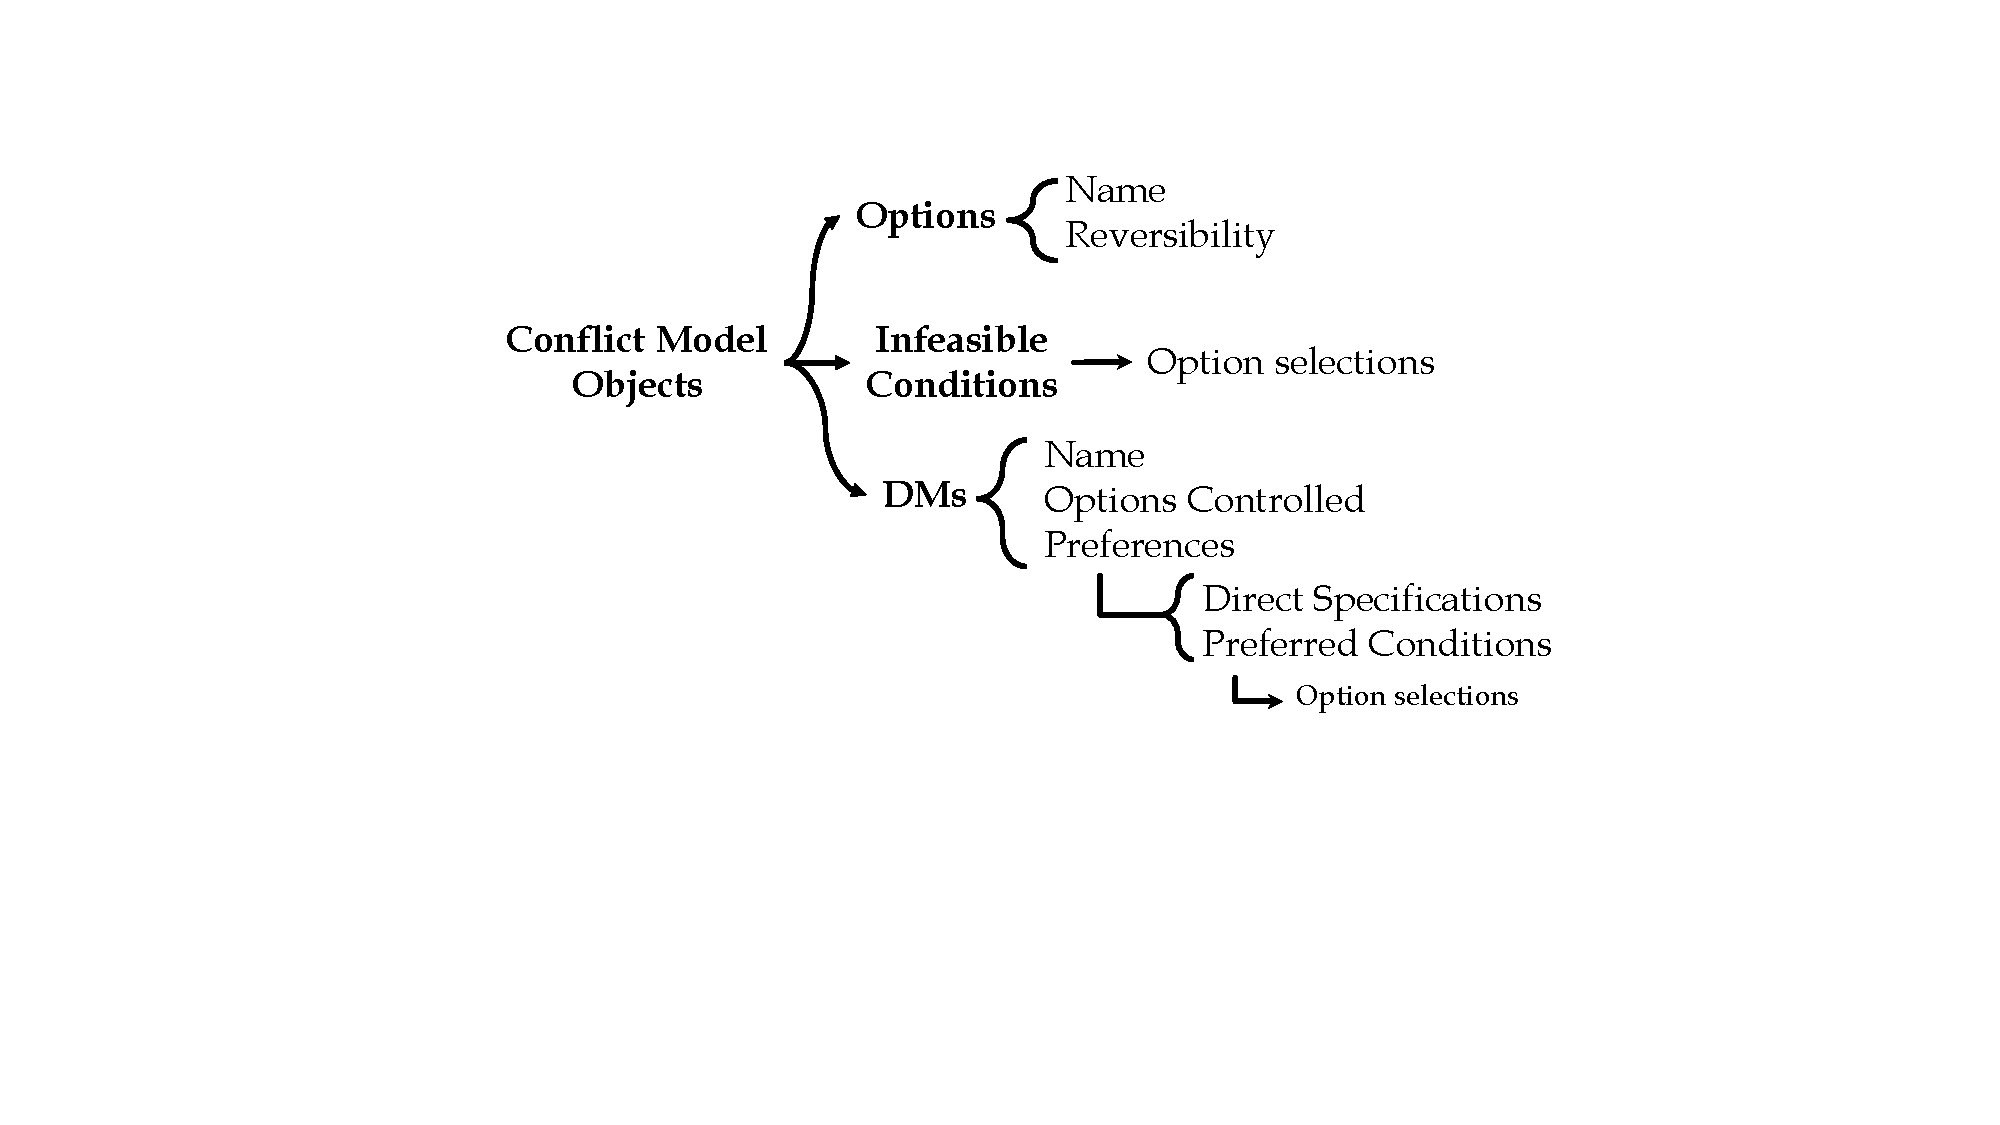
\includegraphics[width=3.5in]{PDF-IMG/DSS/confspecs.pdf}

\caption{Conflict Specifications Hierarchy in GMCR+}

\label{fig:confspecs}
\end{figure}
\end{center}

Typically, DMs are identified before options as discussed in the standard GMCR procedure in Figure \ref{fig:procedure_or}. However, options will be discussed as the root of the conflict model, which better reflects the structure of the DSS. 

\subsection{Option Objects}
Each option within a conflict is represented by an object. This object contains all of the defining attributes as follows:
\subsubsection{Option Name}
A simple human readable identifier used while modeling the conflict and when displaying results.
\subsubsection{Reversibility}
An option may be On or Off (selected or not). An option is reversible if it is permissible to move back and forth between the two option selections. An option is irreversible if it is  permissible to move in only one of these directions.


A list containing all of the options within a conflict is part of the top-level specification of that conflict.  References to the option objects contained within that master list appear in three instances: 
\begin{itemize}
\item DM objects (to allow a DM to have control over an option)
\item Infeasible conditions (making a condition dependent on option selections)
\item Preferred conditions (within a DM's preferences) 
\end{itemize}

\noindent The last two instances will be clarified in the following subsection.

\subsection{Condition Objects}
\label{sec:condition}
A group of option selections is called a condition. For example, consider a model of five options. The complete set of states where no option selection is made could be represented as ``- - - - -". A pattern in which the second option is chosen and the fourth option is not chosen is described as ``- Y - N -". Conditions of this form are used in the two aforementioned instances: determining infeasible states and specifying preferences using preference prioritization.


\subsection{Infeasible Conditions}
\label{sec:InfeasCond}
A conflict's infeasible states are described through a list of conditions mentioned earlier. All states for which one or more of the infeasible conditions is true are removed from the model before analysis is carried out.  Specifying the infeasible states in a conflict through the use of infeasible conditions allows a large number of related infeasible states to be described more easily.

\subsection{DM Objects}
Each DM within a conflict is represented by an object. This object contains all of the defining attributes of the DM as follows:
\subsubsection{DM Name}
A simple human readable identifier used while modeling the conflict and when displaying results.

\subsubsection{Options Controlled}
A list of references to options (contained in the top level specifications) that the DM controls. Each option is controlled by one and only one DM. 
\subsubsection{Preferences}
This refers to the ordering of conflict states from most preferred to least preferred for each DM. This information can be input using direct specification or using preference prioritization conditions. GMCR+ represents preferences by assigning payoff values to each state for each DM. A higher payoff value indicates a greater preference for that state by that DM. A user can directly specify preferences by providing a list of all states, ordered from most preferred to least preferred.  Equally preferred states can be indicated by grouping them together with brackets and the DSS will then assign payoffs accordingly.

Another way to specify preferences is a qualitative tool utilizing the preference prioritization method that uses preferred conditions. When using preference prioritization to assign payoffs, preferred conditions are specified for each DM.  These conditions are ordered from the most preferred conditions to the least preferred conditions.  Weights are assigned to each of the conditions, and a state's payoff is calculated by summing the weights of all conditions it satisfies.



\section{Conflict Data Processing}
\label{sec:ConfData6}
In this section, algorithms and pseudocodes for how GMCR+ process the aforementioned conflict specifications are outlined. 
\subsection{Removing Infeasible States}
\label{sec:RemInfes}
Infeasible states must be removed from a conflict before useful analysis can be performed.  Since infeasible states are represented through conditions, the list of feasible states can be obtained through a subtraction process.

A condition with no option selection specified (i.e. all possible options can be either taken or not) is referred to as a ``null condition".  A null condition includes the complete set of mathematically possible states (given by the expression $2^m$ where $m$ is the number of options in a conflict model). The list of feasible states in a conflict model can be expressed as a set of conditions. Starting with the null condition, the list of conditions that describe the feasible states of a game can be obtained through Algorithm \ref{alg:feasible}. Please note that Algorithm \ref{alg:x-y} is called within Algorithm \ref{alg:feasible}. The results provided by the use of these algorithms is the set of feasible states for the conflict, referred to as $F$.


\begin{algorithm}
\caption{Calculate Feasible States}
\label{alg:feasible}
\begin{algorithmic}
\State $F  \leftarrow $ null condition
\State $G \leftarrow $ Set of infeasible conditions
\State $W \leftarrow \phi$
\For{each condition $g$ in G}
	\For{each condition $f$ in F}
		\State $X \leftarrow$ \Call{subtract}{$f,g$}
		\State $W \leftarrow W \cup X$
	\EndFor
	\State $F \leftarrow W$
	\State $W \leftarrow \phi$
\EndFor


\end{algorithmic}
\end{algorithm}


%pseudocode

\begin{algorithm}
\caption{Calculate $X-Y$}
\label{alg:x-y}
\begin{algorithmic}
\Function {Subtract}{x,y}
\If{$X \cap Y = \phi$}
\\
\Return $X$
\EndIf

\State $W = \phi$ 
\For{each option $i$}
	\If{$X[i] \neq $ $'-'$}
		\State $Z \leftarrow X$
		\State $Z[i] \leftarrow ~Y[i]$
		\State $W \leftarrow W \cup Z$
		\State $X[i] \leftarrow Y[i]$
	\EndIf
\EndFor
\\
\Return $W$
\EndFunction
\end{algorithmic}
\end{algorithm}



\subsection{Preference Prioritization}
\label{sec:prefPrioritization}
Preference prioritization is the process by which a ranked list of preferred conditions can be translated into payoff values for each state according to each DM. In order to perform the preference prioritization, the first step is to establish a weight for each preferred condition.  Given a user-provided list of conditions, $P$, ordered from most to least important, payoff values can be assigned according to the following procedure:

\begin{itemize}
\item Algorithm \ref{alg:weightconditions} outlines the method used to weigh the conditions in GMCR+. Each condition is given a weight of $2^{\lvert P \rvert - i}$, where $\lvert P \rvert$ is the length of the user provided list of conditions, and $i$ is the position of the condition on the list.
\item After all the conditions have been weighted, all feasible states within the conflict model are then scored against these conditions as outlined in Algorithm \ref{alg:scorestates}. The payoff for a state according to each DM is the sum of the weights of all conditions that are satisfied by the state.
\end{itemize}
\noindent As each DM has a unique set of preferred conditions, which will yield unique payoff values for each state, this procedure must be performed for every DM.
 

\begin{algorithm}
\caption{Weigh Preferred Conditions}
\label{alg:weightconditions}
\begin{algorithmic}
\State $P=$ User-Provided list of Preferred Conditions
\For{each condition $p$ in $P$ and index $i$ in $\lvert P \rvert$} \Comment{ $\lvert P \rvert$ \it{is the length of the user provided list}}
	\State $p.weight \leftarrow 2^{\lvert P \rvert-i}$ \Comment{\it{p.weight is the weight of the condition $p$}}
\EndFor
\end{algorithmic}
\end{algorithm}

\begin{algorithm}
\caption{Score States}
\label{alg:scorestates}
\begin{algorithmic}
\State $ F = $ List of Feasible States
\State $ P = $ User-Provided list of Preferred Conditions
\For{state $f$ in $F$}
	\State $f.$payoff$ \leftarrow 0$
	\For{condition $p$ in $P$}
		\If{$f$ satisfies $p$}
			\State $f.$payoff$ \leftarrow f.$payoff$+p.$weight
		\EndIf
	\EndFor
\EndFor

\end{algorithmic}
\end{algorithm}


\subsection{Direct Ranking Handling}
\label{sec:DirectRanking}
An alternative method for specifying preferences is through direct specification. Direct specification is the manual ordering of states from the most preferred to least preferred state for each DM. The user-entered preference rankings are converted to payoff values using Algorithm \ref{alg:convertpref}.

\begin{algorithm}
\caption{Convert Preference Ranking to Payoff Values}
\label{alg:convertpref}
\begin{algorithmic}
\State $R \leftarrow$ User-entered preference ranking
\For{each state number $r$ in $R$ and index $i$ in $\lvert R \rvert$} 
	\State $r.$payoff$ \leftarrow \lvert R \rvert - i$
\EndFor

\end{algorithmic}
\end{algorithm}

\subsection{Reachability Matrix}
The reachability matrix contains information central to all analysis capabilities of the GMCR+ system.  For each DM, an $\lvert F \rvert \times \lvert F \rvert$ reachability matrix is constructed, where $\lvert F \rvert$ is the number of feasible states in the conflict model. If state $j$ is reachable from state $i$ by a DM, then entry $[i,j]$ of the reachability matrix for that DM is assigned the payoff of state $j$ for that DM.  If state $j$ is not reachable from state $i$ by a DM, then the $[i,j]$ entry is undefined. Figure \ref{fig:reachMatrix} is an example for a 3-state model where a DM has a move from state $s_1$ to state $s_2$ that has a payoff of 3. On the other hand, a move from state $s_2$ to state $s_3$ has a payoff of $-5$. There is no possible move from state $s_3$ to state $s_1$, but a move from state $s_1$ to state $s_3$ has a payoff of 1 and the move is irreversible.

\begin{center}
\begin{figure}[h!]
\centering
\includegraphics[scale=0.55]{PDF-IMG/DSS/matrix_reachable_dem.pdf}

\caption{Reachability Matrix Example}

\label{fig:reachMatrix}
\end{figure}
\end{center}

Using this format allows both reachability and payoff information to be co-located and used in different GMCR+ procedures and analyses.

\section{Analysis Engines}
\label{sec:Engine}

GMCR+ utilizes both logical and matrix approaches to determine and calculate the stability of states. This allows the system to extract insightful information while being fast and efficient in analyzing conflict models.

The Logical Solution Engine in GMCR+ calculates the stability  of each state for every DM according to the four solution concepts introduced in Section \ref{sec:stability}: Nash, SEQ, GMR, and SMR. Overall conflict equilibria can be determined based on individual stabilities. Moreover, the engine can generate a narration of the stability for any given state and DM. This insightful narration provides a clear picture of what sanctioning moves or unilateral improvements (UIs) are directly responsible for the stability or instability of a state.  

In addition to the Logical Solution Engine, the back end of the system utilizes the Matrix Approach by Xu et. al. \cite{xu2007matrix,xu2009}. The advantage of using the Matrix Approach is the increased computational speed due to the efficiency of computers when dealing with matrices versus logical loops. However, if the user demands insights for a specific state, then the logical approach is utilized to provide the narration.

Finally, a subsystem to utilize the above engines is implemented to incorporate Inverse GMCR. Inverse GMCR is a new extension to the original GMCR \cite{rami2012smc,SMC2013Rami,GDN2013Rami} in which GMCR is utilized as a negotiation tool rather than a prediction tool. Through the application of the stability concept definitions and analysis of the reachability matrix, it is possible to generate a list of conditions that must be satisfied by the DMs' preferences to lead to an equilibrium at a given state. The engine can produce a list of the conditions that must be satisfied to produce an equilibrium under any of the basic stability concepts: Nash, SEQ, GMR, and SMR.
%pseudocode - same question as under logical engine




\section{Graphical User Interface}
\label{sec:GUI}
The GUI for GMCR+ was created in python, using the \textit{tkinter} user interface package. The basic interface, shown in Figure \ref{fig:screen1}, includes a large navigation bar at the top of the screen.  This bar displays each of the logical steps in the modeling of a conflict, and allows the user to easily move between them. At the top left of the screen, the user can find standard utility buttons to load, save, and create new conflict models.
The remainder of the screen is used to display and edit information related to the active step of the modeling process.  To the right edge of the screen, a column provides a quick reference about  the current step of the modeling process and how to use the interface.

\begin{center}
\begin{figure}[h!]
\centering
\includegraphics[width=\textwidth]{PDF-IMG/DSS/Screens/Screen1.jpeg}

\caption{GUI for GMCR+}

\label{fig:screen1}
\end{figure}
\end{center}


\subsection{Decision Makers and Options}
This is the first step in conflict modeling where the user or analyst defines the DMs and their options in the conflict. The full list of DMs in the conflict is shown to the left of the screen as shown in Figure \ref{fig:screen11}. Clicking on a DM's name will select it, displaying the DM's associated options in a list to the right. While a DM or option is selected, it can be deleted, or its name can be modified. Buttons at the bottom of the screen allow the order of DMs and options to be changed, and new DMs or options to be added to the conflict. The information panel at the right edge of the screen displays the number of defined DMs, options, and the total number of states that would be in the game if no infeasible states were removed.

\begin{center}
\begin{figure}[h!]
\centering
\includegraphics[scale=0.55]{PDF-IMG/DSS/Screens/Screen11.jpeg}

\caption{DMs and Options Screen}

\label{fig:screen11}
\end{figure}
\end{center}


%should controls be mentioned? (double click to edit/create new, keyboard shortcuts, etc.)
\subsection{Infeasible States}
After defining DMs and options, the program will generate a list of all possible states. There are usually infeasible states that need to be removed as explained earlier in Sections \ref{sec:InfeasCond} and \ref{sec:RemInfes}. The infeasible states screen (Figure \ref{fig:screen2}) allows the user to create conditions specifying infeasible states to be removed.

\begin{center}
\begin{figure}[h!]
\centering
\includegraphics[width=\textwidth]{PDF-IMG/DSS/Screens/Screen2.jpeg}

\caption{Infeasible States Screen}

\label{fig:screen2}
\end{figure}
\end{center}

The panel to the left contains a set of toggle buttons where  option selections can be made to specify an infeasible condition. Clicking ``remove as infeasible condition" will remove all states satisfying this condition from the conflict and display the infeasible condition along with the number of removed states in the middle of the screen. Clicking ``remove as mutually exclusive options" generates a list of conditions prohibiting any states where two or more of the chosen option selections are taken. For example, consider a person with three options: eat, sleep, and breathe. A person can't eat and sleep at the same time. Moreover, a person can't eat or sleep without also breathing. Table \ref{tbl:eatsleep} outlines all possible states combinations for this example. Four states are infeasible in this example: 2, 3, 4, and 8. In order to remove them, an analyst would have to input at least three conditions manually:

\begin{itemize}
\item Eat and sleep
\item Eat and not breathe
\item Sleep and not breathe
\end{itemize} 

However, using the mutually exclusive button, an analyst can generate this list of conditions by selecting Eat, Sleep, and not Breathe and clicking on ``remove as mutually exclusive options".

\begin{center}
\begin{table}[h!]
\centering
\caption{Example for mutually exclusive options}
\includegraphics[scale=0.70]{PDF-IMG/DSS/table_eatsleep.pdf}

\label{tbl:eatsleep}
\end{table}
\end{center}

The feasible states are displayed on the right of the infeasible conditions panel as shown in Figure \ref{fig:screen2}. The set of feasible states can be displayed either as a list of feasible conditions, as a full list of feasible states in YN format, or as ordered and decimal state numbers. On the right edge of the screen, an information panel displays the original number of states in the conflict, the number of states removed, and the number of feasible states remaining. below that is a brief set of instructions for using the interface. 

\subsection{Irreversible Moves}
In this step, an analyst can define the reversibility of each option. In default, all options in the conflict are displayed with a two-headed arrow pointing between `Y' and `N' denoting that all moves are reversible. Clicking the arrow toggles the direction of reversibility.  In this way, the user or analyst can leave the option as reversible, or define the direction of irreversibility. All moves in Figure \ref{fig:screen10} are reversible except that of Air Strike.  


\begin{center}
\begin{figure}[h!]
\centering
\includegraphics[scale=0.55]{PDF-IMG/DSS/Screens/Screen10.jpeg}

\caption{Irreversible Moves Screen}

\label{fig:screen10}
\end{figure}
\end{center}


\subsection{Preferences}
Preferences for DMs can be specified through preferred conditions or through direct ranking of states as mentioned previously in Sections \ref{sec:prefPrioritization} and \ref{sec:DirectRanking}. The preferred conditions method allows the analyst to define preference prioritization conditions to make the ranking of states easier and more intuitive. Direct ranking allows the analyst to fine tune the results from prioritization or assumes the analyst is certain about the ranking of states for each DM. 

\subsubsection{Prioritization}
As explained earlier in Section \ref{sec:condition}, a condition is a set of option selections describing a group of states. By specifying conditions that are preferred by a DM and ordering these conditions by importance, a ranking of states can be generated using the methodology described in Section \ref{sec:prefPrioritization}.

\begin{center}
\begin{figure}[h!]
\centering
\includegraphics[width=\textwidth]{PDF-IMG/DSS/Screens/Screen3.jpeg}

\caption{Preference Prioritization Screen}

\label{fig:screen3}
\end{figure}
\end{center}

The panel to the left of the screen in Figure \ref{fig:screen3} is a table with all DMs and their corresponding preference ranking. Clicking on any DM will change its color to green and allow the preferences for that DM to be modified. A user can click ``Done" to clear the DM selection. The panel in the middle includes toggle buttons for all DMs and their options. In order to add a preferred condition, a user will make option selections and can either add them directly as a preferred condition or move them to a stagging area where multiple condition can be added together with equal weight. The right panel of the screen displays the preferred conditions for the selected DM and the weights associated with those conditions.

A large table displaying the conflict in option form occupies the bottom of the screen in Figure \ref{fig:screen3}. The states are ordered according to their ranking for the active DM. The table also displays the payoff value of each state according to the active DM. If no DM is selected, the states are ordered based on state number and payoff values for all DMs are shown.

\subsubsection{Preference Ranking}
A user may wish to fine-tune the ranking of states after performing preference prioritization or simply entering preference information directly. At the top of the screen in Figure \ref{fig:screen4} is a large button allows a user to enable manual preference ranking.  This is accomplished by modifying the preference rankings shown for the DMs in the fields below. States are listed using their ordered numbers, and equally preferred states can be indicated by enclosing them in square brackets.  In the middle of the screen, a large text box displays feedback on the validity of the entered preference rankings. Each preference ranking must contain each state once and only once to be considered valid.  At the bottom of the screen, an option form table for the conflict is shown, similar to that on the Preference Prioritization screen. If the user wishes to revert changes to preferences made on the direct ranking screen, they can return to the Preference Prioritization screen, and click the large button that appears at the top of the screen.

\begin{center}
\begin{figure}[h!]
\centering
\includegraphics[width=\textwidth]{PDF-IMG/DSS/Screens/Screen4.jpeg}

\caption{Preference Ranking Screen}

\label{fig:screen4}
\end{figure}
\end{center}

\subsection{Equilibrium Results}
\label{sec:EqResultsScreen}
Figure \ref{fig:screen1} illustrates the ``Equilibria Results" screen. The top of the screen shows the results of equilibria calculations for all states and solution concepts in an option form table for the conflict model similar to that on the preferences screens. Moreover, an analyst can examine the equilibria for coalitions by merging possible coalitions in square brackets to the top of the screen. To the right of the screen is the analysis narration panel, which allows an analyst to check for individual stability by selecting a DM, state, and a solution concept and the process used to determine that individual stability or instability is explained. At the bottom of this screen, an option to launch a visualizer is available which is explained in Section \ref{sec:presentation}.

\subsection{Inverse GMCR}
\label{sec:InverseScreen}
This screen deals with one of the novel additions to GMCR as mentioned in the introduction and in Section \ref{sec:Engine}. The screen contains a control panel to the left as seen in Figure \ref{fig:screen5}. This control panel allows the analyst to specify a desired equilibrium state. Furthermore, an analyst can select a preference vary range for each DM and then perform the Inverse GMCR calculations. Required conditions for stability are explained to the right for each solution concept. A Long form results can be displayed on the bottom by selecting to display all permutations in the control panel and can be filtered by the solution concepts check boxes. This is a useful addition allowing analysts to perform extensive sensitivity analysis on preferences.

\begin{center}
\begin{figure}[h!]
\centering
\includegraphics[width=\textwidth]{PDF-IMG/DSS/Screens/Screen5.jpeg}

\caption{Inverse GMCR Screen}

\label{fig:screen5}
\end{figure}
\end{center}

\section{Presentation of Results and Post Analysis Tools}
\label{sec:presentation}
Web technologies present a wide array of opportunities for easy to create and distribute visualizations of information.  The complexities of a conflict's graph model are often most easily understood when presented in a visual form, and so the following tools were created to accompany GMCR+, facilitating presentation and allowing deeper analysis.

\subsection{Graphical Representation}
Within the equilibria results screen described in Section \ref{sec:EqResultsScreen} is a button to launch a visualizer. Clicking this button will launch a web application within the GMCR+ system allowing the analyst to see the actual graph of the conflict model as shown in Figure \ref{fig:screen6}. The default view is a tree diagram illustrating a status quo analysis diagram. The top of the tree denote the status quo and the branches are the possible unilateral moves from that state by each DM. Lines are color and dash coded for each DM. Hovering the mouse on any state shades all states within the tree. 

\begin{center}
\begin{figure}[h!]
\centering
\includegraphics[width=\textwidth]{PDF-IMG/DSS/Screens/Screen6.jpeg}

\caption{Conflict Model Tree Diagram}

\label{fig:screen6}
\end{figure}
\end{center}

Hovering the mouse to the bottom of the screen displays an option form table for the conflict model. Hovering the mouse to the left of the screen shows the display options panel as shown in Figure \ref{fig:screen7}. This panel allows an analyst to change the display method between a tree and a graph diagram. Furthermore, multiple options such as selecting a specific DM, showing UIs only, and specifying the tree depth can be adjusted.  

\begin{center}
\begin{figure}[h!]
\centering
\includegraphics[scale=0.45]{PDF-IMG/DSS/Screens/Screen7.jpeg}

\caption{Display Options Panel for Tree and Graph Diagrams}

\label{fig:screen7}
\end{figure}
\end{center}

Switching to the graph diagram mode will show the actual graph model for the conflict at hand as shown in Figure \ref{fig:screen8}


\begin{center}
\begin{figure}[h!]
\centering
\includegraphics[scale=0.55]{PDF-IMG/DSS/Screens/Screen8.jpeg}

\caption{Conflict Model Graph Diagram}

\label{fig:screen8}
\end{figure}
\end{center}

\subsection{Post Analysis}
This is the last screen in the GMCR+ system as illustrated in Figure \ref{fig:screen9}. In this screen an analyst can specify coalitions within the control panel on the left of the screen, similar to the equilibria results screen mentioned in Section \ref{sec:EqResultsScreen}. In addition, this screen has two main submodules described in the following subsections.


\begin{center}
\begin{figure}[h!]
\centering
\includegraphics[width=\textwidth]{PDF-IMG/DSS/Screens/Screen9.jpeg}

\caption{Post Analysis Screen}

\label{fig:screen9}
\end{figure}
\end{center}

\subsubsection{Status Quo Analysis}
In the control panel, an analyst can choose a specific state to act as a status quo for the conflict and carry out the analysis from it. The middle panel will automatically show the selected state as the top of the tree with a `+' sign to expand the branch. Clicking the `+' sign expands the branch into reachable states and UIs are shaded green. This feature allows the analyst to know if a possible equilibria is reachable from the status quo and whether it is reachable solely by UIs. This information is also given in the narration panel to the right of the screen. 

\subsubsection{Goal Technique}
This tool is an extensive version of the Inverse GMCR mentioned in Section \ref{sec:InverseScreen}. An analyst can experiment scenarios by setting particular states to be stable while avoiding other states. Whether these choices are possible or not is explained in the right panel and how they can be achieved if possible is narrated as well.


\section{Case Study: Cuban Missile Crisis}
\label{sec:example}
In order to illustrate the capabilities of GMCR+, an international political conflict is summarized and then analyzed using GMCR+. 

\subsection{Background}
The Cuban Missile Crisis between the United States (US) and the Union of the Soviet Socialist Republics (USSR) in October 1962 is used to demonstrate the capabilities of the DSS GMCR+ \cite{CubanOnline,ben2002cuban,fraser1984,Hipel2011C2Journal}. The crisis was the closest that the USSR and US came to nuclear conflict, but it was averted due to the control and intelligence of the DMs on both sides. After Fidel Castro overthrew the Batista regime in 1959, there was impounding of American property in Cuba, which caused the US to sponsor the Bay of Pigs invasion in April 1961. This was a failed attempt at destroying the perceived military threat, following which the US vowed not to commit military invasion of Cuba. 
In October 1962, US intelligence discovered several USSR missile construction sites including medium-range and intermediate-range ballistic nuclear missiles (MRBMs and IRBMs) on Cuban soil, thus beginning the Cuban Missile Crisis. US President Kennedy summoned the Executive Committee of the National Security Council to advise and consider options to resolve the crisis. The options put forward by the various political and military decision makers included air strike to destroy the missiles, a naval blockade of USSR military ships to Cuba, and more passively stern warning to Cuba and USSR. 
On the other hand, the USSR DM Premier Nikita Kruschev had to consider the options of withdrawing missiles from Cuba or escalating the crisis by attacking US naval blockades, bombing in-range US targets from Cuba, and initiating Intercontinental Ballistic Missile (ICBM) attack on the US. 
The options chosen by both DMs demonstrate an effort to promote the diplomatic channel, as the US chose to blockade USSR military supplies to Cuba while the USSR chose to withdraw the nuclear missiles. On November 20, 1962, with the end of the US naval blockade of Cuba, the Cuban Missile Crisis was finally over.

\subsection{Modeling the Cuban Missile Crisis}
\subsubsection{DMs and Options}
There are 2 main DMs in the Cuban Missile Crisis, the US and the USSR, as seen in the left-hand column of Table \ref{tbl:cuban_table}. Cuba is not modeled as a DM since it does not control any options over the US or the USSR and is not significant to the conflict. The DMs control two options each; the US controls the option of 1) conducting air strike (Air Strike) on Cuba and 2) applying a naval blockade of USSR military ships to Cuba (Blockade). The USSR controls the option of 1) withdrawing missiles from Cuba (Withdraw) and 2) escalating the crisis (Escalate). The same modeling is applied for the crisis studied by Fraser and Hipel \cite{fraser1984} using conflict analysis. Throughout the paper, all screen-shots were taken for this specific conflict. Defining DMs and options is done in the first screen as shown in Figure \ref{fig:screen11}.

\subsubsection{Infeasible states and Irreversible Moves}
Through the various combinations of all options for both DMs, there are a total of 16 possible states; however, 4 states are infeasible where a DM chooses contradictory options. For example, there are no states where the USSR chooses both to Withdraw and to Escalate. Figure \ref{fig:screen2} shows how this step can be implemented in GMCR+. The result is 12 feasible states as shown in the 12 columns in Table \ref{tbl:cuban_table}, with `Y' denoting `yes' indicating an option is taken and `N' denoting `No' indicating an option is not taken. Notice that at state 7, the US choses not to conduct air strike but instead apply a naval blockade to Cuba. Also in state 7, the USSR choses the option of withdrawing missiles and not escalating the crisis. Historically, this was the actual resolution to the crisis where the final equilibrium of the conflict reached. For feasible states, a DM can choose to cause a unilateral transition between states by changing the option choice except if the option is irreversible like the option of an Air Strike by the US as illustrated in Figure \ref{fig:screen10}.
 
\begin{center}
\begin{table}[h!]
\centering
\caption{DMs, Options and Stated for the Cuban Missile Crisis }
\includegraphics[scale=0.70]{PDF-IMG/DSS/cuban_table.pdf}

\label{tbl:cuban_table}
\end{table}
\end{center}

\subsubsection{Preferences}
In order to rank states for a DM, one can directly rank the states using pairwise comparisons of feasible states. However, this process can be inaccurate and lengthy. Hence, an efficient process is necessary. 

Table \ref{tbl:CubanPrefTbl} demonstrates preference statements for the US in the Cuban Missile Crisis. These preference statements are used to rank the states based on the algorithms described in Section \ref{sec:prefPrioritization}. For example, preference statement with the highest ranking, statement \#1, means that the US would most prefer the USSR to just withdraw their missiles from Cuba. The seventh US preference statement means that the US prefers an air strike or a blockade if the USSR does not withdraw and does not escalate. Figure \ref{fig:screen3} shows how to input these statements into GMCR+. Through algorithms in GMCR+, the preference statements are automatically converted to states rankings.


\begin{center}
\begin{table}[h!]
\centering
\caption{US Preference Statements}
\includegraphics[scale=0.70]{PDF-IMG/DSS/CubanPrefTbl.pdf}

\label{tbl:CubanPrefTbl}
\end{table}
\end{center}

\subsubsection{Equilibria Results and Insights}
The equilibria results screen depicted in Figure \ref{fig:screen1} shows that states 5, 6, and 7 are the strongest equilibria for this conflict model. State 7 was historically the final resolution of the conflict. Launching the visualizer at the bottom of the screen reveals both tree diagram and the graph model of the conflict depicted in Figures \ref{fig:screen6} and \ref{fig:screen8}. Note that solid lines indicate US while dashed lines indicate the USSR.

Using the post analysis screen, one can see that state 7 is reachable from the status quo state 1 and is reachable solely by UIs. Furthermore, the analyst may wish to carryout some sensitivity analysis using the Inverse GMCR screen as in Figure \ref{fig:screen5}.

\section{Summary of Features}
Summary of GMCR+ features with a comparison of different DSSs tailored for GMCR is illustrated in Table \ref{tbl:DSScomparison}. It is very clear that GMCR+ is richer that all of its predecessors and superior in performance. 

\begin{center}
\begin{table}[h!]
\centering
\caption{Comparison of different DSSs capabilities}
\includegraphics[scale=0.73]{PDF-IMG/DSS/DSS_Comparison_Table.pdf}

\label{tbl:DSScomparison}
\end{table}
\end{center}

\subsection{Overall review}

In summary, three essential elements constitute the GMCR+ DSS. The structure of the model (conflict specifications), conflict data processors, and display components (GUI).

The conflict specification is built on a structured set of objects (options, DMs, conditions, etc.) with defined properties and interactions that exist within a conflict model as outlined in Section \ref{sec:ConfSpecs5}.

The ``conflict data processors" as explained in Sections \ref{sec:ConfData6} and \ref{sec:Engine} constitute the solution engines. GMCR+ has 4 distinct and independent ``solvers": the logical solver, the matrix solver, the inverse solver, and the goal seeker.

The GUI is the component which the user actually interacts with. The purpose of the GUI is to control the flow of all parts of the program.  It is organized into screens, of which there are eight so far (more can be easily added).  Each of these screens is composed of a series of smaller elements that display and/or control some elements of either the conflict model or one of the solution engines. These elements are reusable on multiple screens, as appropriate. When a user launches the program, the basic parts of the user interface are constructed, then an empty conflict model is formulated. GMCR+ then initializes all the parts of the interface that are meant to contain and/or control conflict information by building those elements and giving them references to the part of the conflict model they are meant to represent. When a user interacts with a part of the interface, it sends a message to the conflict model and the requested change is executed.  This change is then reflected in all other elements of the interface that hold references to that part of the conflict model.

When a user navigates to one of the result screens (Equilibria Results, Inverse GMCR, or Post Analysis), GMCR+ creates an instance of one of the solvers, giving it a reference to the current conflict model.  The solver does the work of interpreting the conflict model and generating results.  The interface elements of the screen (some of which communicate with the conflict model, some with the solver, while others communicate to both) display the results generated. Moreover, it allows the user to request the solver for additional analysis, the results of which are returned to the appropriate user interface element.

Figure \ref{fig:elemntss} illustrates the different elements of GMCR+ and their interactions.


\begin{center}
\begin{figure}[h!]
\centering
\includegraphics[width=\textwidth]{PDF-IMG/DSS/Leggo.pdf}

\caption{Different elements of GMCR+ and their interactions}

\label{fig:elemntss}
\end{figure}
\end{center}



\subsection{Future Work}

There are recent and ongoing expansions of the GMCR methodology which can be conveniently incorporated into GMCR+ due to its modular design. These expansions include:
\begin{itemize}
\item Strength of preference \cite{hamouda2004strength,hamouda2006strength}
\item Unknown preferences  \cite{li2004}
\item Fuzzy preferences \cite{bashar2012fuzzy,hipel2011fuzzy}
\item Grey-Based preferences \cite{kuang2013grey}
\item Hypergames \cite{Bennett1980HYPER,Wang1988Hyper}
\end{itemize}

Figure \ref{fig:elemntss} depicts the modular design of GMCR+ and how new extensions can be integrated.

\section{Conclusions}
The framework, modules, and algorithms used within the newly developed DSS called GMCR+ is presented in this paper. It is evident how GMCR+ allows the analyst to be accurate, efficient, and insightful in modeling and analyzing strategic conflicts. The presentation and visualization within GMCR+ provide a superior platform to communicate the conflict dynamics and results. Strategic insights are derived from the rich and easy to manipulate post-analysis tools provided within the system. Finally, the flexibility and modularity taken into account makes this system adaptable and open for future theoretical developments in the field of conflict resolution.


%%%%%%%%%%%%%%%%%%%%%%%%%%%%%


\section{Chapter Summary}

%======================================================================
\chapter{Conclusions}
In addition to the methodologies presented in this proposal, several important topics are outlined in the following sections and will be investigated. These topics fall within third party modeling in conflict resolution.
%\section{Third Party Strategy Recommendations}
Various third party roles and strategies are investigated and presented in Chapter 2 of this proposal. A methodology is needed to determine the best role and strategy that a mediator should undertake in any particular conflict situation. The motivation to introduce such a methodology is to operationalize the notion of third party intervention.

%\section{Enhance the Inverse Approach Methodology}
Although basic features of the inverse approach are outlined in this proposal, further enhancements are planned to extend the capability and usefulness of the methodology. One area being studied is the development of a cost and payoff extension to the inverse approach to GMCR. This feature will allow for narrowing down the list of possible profiles and will allow for more relevant and meaningful results.

%\section{Inverse Status Quo Analysis}
An inverse approach to determine the required starting points in order to attain desired equilibria will be investigated. This will be achieved by tracking the evolution of the conflict backward from a desired equilibrium to the status quo states.


%\section{In-Depth Sensitivity Analysis}
As mentioned earlier, with the introduction of the inverse approach, a more in-depth model for sensitivity analysis that determines the robustness of any equilibrium by outlining the range of preference profiles in a conflict will be put forward. 

%\section{Decision Support System}
Work has already started on a new decision support system using both the logical and matrix approaches for GMCR calculations. The new decision support system has the capability to perform basic inverse approach calculations using the definitions presented herein. In addition, the software will have the capability to perform regular and inverse status quo analysis. It should be noted that extensions made to the graph model for conflict resolution can be easily embedded into the new decision support system.

%\section{Application to Real World Conflicts}
In order to better understand and appreciate the insights of the proposed methodologies, real world examples will be analyzed and investigated. The intention is to apply the methodologies to different conflict types, including political, environmental, and business conflicts.
%\section{Timeline}
The research goals and approximate completion dates are summarized and outlined in Table \ref{tbl:milestones} below.
\begin{table}[H]
\centering
\includegraphics[scale=.8]{PDF-IMG/Research_Milestones.pdf}

\caption{Research Milestones and Schedule}

\label{tbl:milestones}
\end{table}
%======================================================================


%----------------------------------------------------------------------
% END MATERIAL
%----------------------------------------------------------------------

% B I B L I O G R A P H Y
% -----------------------

% The following statement selects the style to use for references.  It controls the sort order of the entries in the bibliography and also the formatting for the in-text labels.
\bibliographystyle{apalike}
% This specifies the location of the file containing the bibliographic information.  
% It assumes you're using BibTeX (if not, why not?).
\cleardoublepage % This is needed if the book class is used, to place the anchor in the correct page,
                 % because the bibliography will start on its own page.
                 % Use \clearpage instead if the document class uses the "oneside" argument
\phantomsection  % With hyperref package, enables hyperlinking from the table of contents to bibliography             
% The following statement causes the title "References" to be used for the bibliography section:
\renewcommand*{\bibname}{References}

% Add the References to the Table of Contents
\addcontentsline{toc}{chapter}{\textbf{References}}

\bibliography{uw-ethesisB}
% Tip 5: You can create multiple .bib files to organize your references. 
% Just list them all in the \bibliogaphy command, separated by commas (no spaces).

% The following statement causes the specified references to be added to the bibliography% even if they were not 
% cited in the text. The asterisk is a wildcard that causes all entries in the bibliographic database to be included (optional).

%\nocite{*}

\end{document}
